\section{Introduction}
\todo{rename patient to bci user and participant}

Communication BCIs have a target population consisting of patients in various
stages of paralysis or \ac{lis},
severe motor impairment
\todo{cite and discuss Usability and Workload of Access
Technology for People With Severe Motor
Impairment: A Comparison of Brain-
Computer Interfacing and Eye Trackin}

often suffering from oculomotor impairments.
can introduce problems in bci ~\cite{Brain-computer interface (BCI) evaluation
in people with amyotrophic lateral sclerosis}, discuss als example

\todo{. As with eye tracking SGDs, visual
and oculomotor impairments may limit PALS’s performance
with visual BCI systems (Fried-Oken et al., 2020). Although
}

\cite{FriedOken2020}

This reduces their performance operating visual oddball \ac{bci}s (see
section\todo{ref section} for an overview), since they
are presumed unable to comfortably redirect their gaze at the desired target,
i.e., perform overt \ac{vsa}.\todo{cite some visual gaze-independent bci}
They might more naturally operate in covert \ac{vsa}, where the gaze and
\ac{vsa} do not coincide.
Several studies show that performance drops when not fixating the intended
target~\cite{Brunner2010, Frenzel2011, Treder2010, RonAngevin2019,
VanDenKerchove2024}, necessitating gaze-independent solutions.

Usually, they aim to improve gaze-independent \ac{bci} by optimizing
performance in cued covert \ac{vsa}.
These studies build on the assumption that patients with eye motor impairment
would feel comfortable operating an interface in pure covert \ac{vsa} with
central fixation.
One could argue that a \ac{bci} that is only verified to work when a central
fixation is maintained, could also be considered gaze-dependent.
This does not account for the residual eye motor capabilities of most severly
paralyzed or locked-in patients and the comfort they experience while
performing the gaze fixation.

Our previous study, presented in chapter \todo{ref chapter}  partially tried to account for this
and showed gaze-independent performance can be improved
improved in healthy subjects using a suited decoding strategy.
Yet, there is a strong need for verification of results obtained in healthy
samples.
It is a striking constatation that studies reporting on
gaze-independent visual \ac{bci} in patients that are actually eye-motor
impaired are very few.
in patients, cite different characteristics, differences
in setting, environment and equipment,
\todo{List conclusions of Peters2020 (severely eye motor impaired als patients
able to use a hex-o-spell)}
\todo{discuss Lesenfants2014}
\todo{discuss Marchetti2013}

Eventually, one of the end goals of this research line is to develop
gaze-independent \ac{bci} for patients that
are fully locked-in and have no option left than to use a \ac{bci}.
However, this group is very small and it is often a challenge to recruit them
into a study and perform experiments with them~\cite{Wolpaw2006}.
Patients with less severe paralysis or in less progressed disease stages that struggle with
eye-tracking technology could also benefit from
solutions tailored to their specific situation.

Therefore, we aim to apply the concepts from earlier work an literature to
patients with various degrees motor impairment and various
degrees of eye motor impairment.
The objectives of this case study are as follows:
\begin{enumerate*}
  \item Explore capabilities and experienced comfort of eye motor impaired
    patients,
  \item evaluate the performance of a gaze-independent visual \ac{bci} in patients
  \item verify if this performance can be improved with a suitable decoding
    strategy.
\end{enumerate*}


\section{Materials \& methods}
\subsection{Patient recruitment}
Patients were recruited from across the Neuromuscular Reference center at
University Hospital Leuven (Leuven, Belgium), TRAINM Neuro Rehab Clinics
(Antwerp, Belgium), the Neurorehabilitation Unit at University Hospital Lille
(Lille, France) and a specialized care home (France).
Experiments were performed under the supervision of their treating physician.
Patients were recruited based on the following criteria.
To qualify for inclusion, patients must
\begin{enumerate}
	\item be at least 18 years old and no older than 60
	years,
  \item belong to class 2 or 3 according the \ac{bci}	patient selection criteria
    presented by~\textcite{Wolpaw2006},\label{item:patients/inclusion/wolpaw}
  \item have limitations to the extent or comfort of their eye motor control\label{item:patients/inclusion/oculomotor}
\end{enumerate}
Patients were excluded if they
\begin{enumerate}
  \item have a diagnosis of a major medical condition, including any major
    neurological or psychiatric disorder other than those of interest based on
    inclusion criteria~\ref{item:patients/inclusion/wolpaw}
    and~\ref{item:patients/inclusion/oculomotor}\label{item:patients/exclusion/medical}
  \item have a predisposition to or have a history of any kind of epileptic seizures,
    including photosensitive epilepsy,\label{item:patients/exclusion/epilepsy}
  \item have a severe loss in vision or hearing, that would significantly impair
        participation in the experiment,\label{item:patients/exclusion/vision}
  \item are currently using specific psychoactive medications or substances that could affect the out-
        come.\label{item:patients/exclusion/cognitive}
  \item be able to understand the experiment instructions and cooperate,
  \item have any other limitations preventing them from performing the given task.
\end{enumerate}

In total, 11 patients were contacted, of which 1 \ac{ms} patient was excluded based on
criterion~\ref{item:patients/exclusion/vision}, 1 \ac{tbi} patient on
both~\ref{item:patients/exclusion/epilepsy}
and~\ref{item:patients/exclusion/cognitive}, and one stroke patient based
on~\ref{item:patients/exclusion/medical}
One further stroke patient was excluded due to technical
difficulties during the experimental session.
Vision was assessed using a LogMAR chart~\cite{Bailey1976}.

Ultimately, 7 patients were retained.
Of these, one patient was diagnosed from bulbar-onset \ac{als}.
\ac{als} is a neurodegenerative disease affecting the motor neurons, leading to
progressive loss of motor function.
This initially results in general weakness and loss of muscle tone, but
eventually results in full body paralysis.\todo{cite}
Although speech and especially eye movements are usually preserved until the
later stages of the disease progression, the bulbar-onset variant is
characterized by an early loss of speech and an increased involvement of eye
motor symptoms~\cite{Guo2022}\todo{which?}.
Furthermore, one of the goals of \ac{bci} is to support \ac{als} patients whose
life span has been extended with life support with and assistive technology to
ensure quality of life.
In these very progressed stages of \ac{als}, eye movement will eventually also
be affected~\cite{Hayashi1991}.

Three other patients were diagnosed with \ac{fa}, a neurodegenerative
disease affecting the
spinal cord, peripheral nervous system and cerebellum.
\ac{fa} results in an impairing loss of muscle coordination.
In progressed stages, the disease can present with nystagmus, saccadic
intrusions and gaze dysmetria~\cite{Cook2017}.

The final three patients were stroke patients.
Brain stem and cerebellar stroke can often lead to forms of \ac{lis}, and
various eye motor disorders are common depending on the exact location
~\cite{Bogousslavsky1987, Moncayo2009}.
Stroke can lead to some of the more severe impairments like ophthalmoplegia or
partial ophthalmoplegia immediately from onset.

Table~\ref{tab:patients/patients} lists the included patients and their
diagnoses.

\todo{check Usability and Workload of Access Technology for People With Severe
Motor Impairment: A Comparison of Brain-Computer Interfacing and Eye Tracking}

\begin{table}[t]
  \centering
  \footnotesize
  \begin{tabular}{llllllllr}
  \toprule
  \textbf{ID}  & \textbf{Age} & \textbf{Sex} & \textbf{Hand.} &
  \textbf{Diagnosis}
  & \textbf{Speech}     & \textbf{Trach.} & \textbf{Communication}          &
  \textbf{Cls.} \\ \midrule
  PA1 & 58  & M   & L     & bulbar-onset \acs{als} & anarthric  & no          & tablet                 & 3  \\
  PB1 & 41  & M   & L     & \acs{fa} & dysarthric & no          & verbal                 & 3  \\
  PB2 & 43  & F   & R     & \acs{fa} & dysarthric & no          & verbal                 & 3  \\
  PB4 & 48  & M   & R     & \acs{fa} & dysarthric & no          & verbal                 & 3  \\
  PC2 & 43  & M   & R     & brainstem stroke & anarthric  & yes         & \makecell[l]{prompting\\+eye movement} & 2 \\
  PC3 & 43  & F   & R     & brainstem stroke & anarthric  & yes         & letterboard            & 2 \\
  PC4 & 54  & M   & R     & \makecell[l]{left cerebellar stroke \\ (trombosis of the basilar artery)} & anarthric  & yes & letterboard & 2 \\
  \bottomrule
\end{tabular}

  \caption[Presentation of included patients including their diagnosis and
  capabilities.]{Presentation of included patients including their diagnosis and
  capabilities.
  (Trach.: patient underwent a tracheotomy, Cls.: classification according
  to~\textcite{Wolpaw2006}).
  }
  \label{tab:patients/patients}
\end{table}
\todo{Replace with classification according to 40. Kübler A, Birbaumer N.
Brain-computer interfaces and communication in paralysis: extinction of goal
directed thinking in completely paralysed patients? Clin Neurophysiol.
2008;119:2658-2666.}
\todo{include year of diagnosis}

\subsection{Eye tracking and eye motor examination}

Self-reported eye motor abnormalities were recorded.
Patients were asked for, the paralysis or inability to move in a given
direction of one or both eyes, the inability to pursue an object to specific
positions, discomfort or fatigue fixating at specific positions or in general
when performing visual tasks and eye tremors while fixating, resting or
pursuing.

Self-reported according to cite.
Additionally, the participants were asked if they experienced any tremors like
nystagmus or other (larger) involuntary eye movements.

Additionaly, we implemented and performed the automated NeuroEye eye movement
test proposed by~\textcite{Hassan2022}.
This test is based on calibration-free eye tracking.
\todo{say which part we used and which part not}
\todo{motivation and text and references Juliette}
\todo{Limited in what it can tell us (check paper)}
\todo{include eye test document juliette}
Table~\ref{tab:patients/eye} details their eye motor impairments and vision of
included patients.
Patient PA1 had the mildest impairment, only reporting fatigue when fixating
for prolonged times.
Eye motor function of subjects PC2 and PC3 were most severly affected.
Patient PC2 was only able to look up and down, and patient PC3 only retained
partial movement of the right eye, while the left eye was permanently closed.

\begin{table}[t]
  \centering
  \footnotesize
  % \begin{tabular}{lll}
%  \toprule
%  \textbf{ID} & \textbf{Oculomotor impairment} & \textbf{Vision (LogMAR)} \\ \midrule
%  PA1  & fixation fatigue & 0.0 \\
%  PB1  & impaired pursuit, fixation fatigue, fixation discomfort, tremor & 0.0 \\
%  PB2  & fixation fatigue, fixation discomfort, tremor & 0.6 \\
%  PB4  & impaired pursuit, fixation fatigue, fixation discomfort, tremor & 0.2 \\
%  PC2  & \makecell[l]{partial ophthalmoplegia (up-down preserved), \\ fixation
%  fatigue, fixation discomfort, tremor} & \makecell[l]{0.0, diplopia corrected \\ with prism glass)} \\
%  PC3  & \makecell[l]{right ophthalmoplegia, left partial ophthalmoplegia, \\ fixation fatigue, fixation discomfort, tremor} & 0.7, right eye closed \\
%  PC4  & deviation of the left eye & 0.6 \\
%  \bottomrule
%\end{tabular}
\footnotesize
\let\oldarraystretch\arraystretch
\renewcommand{\arraystretch}{2}
\newcommand{\skill}{\cellcolor{lightgray}}
\newcommand{\noskill}{\cellcolor{accent1}\textcolor{muteblack}{\BigCross}}
\newcommand{\snoskill}{\cellcolor{accent2}\textcolor{muteblack}{\BigDiamondshape}}
\begin{tabular}{r|ccccccc}
                          & PA1      & PB1      & PB2       & PB4      & PC2       & PC3       & PC4 \\ \hline
  Visual fixation         & \noskill & \noskill & \noskill  & \noskill & \noskill  & \noskill  & \noskill \\
  Eyelid function         & \skill   & \skill   & \skill    & \skill   & \noskill  & \noskill  & \skill \\
  Ocular motility         & \skill   & \noskill & \skill    & \noskill & \snoskill & \snoskill & \noskill\\
  Binocular vision        & \skill   & \skill   & \skill    & \skill   & \noskill  & \snoskill & \snoskill \\
  Field of vision         & \skill   & \skill   & \skill    & \skill   & \skill    & \noskill  & \noskill \\
  Involuntary movement    & \skill   & \noskill & \noskill  & \noskill & \noskill  & \noskill  & \skill \\ \hline
  Visual acuity   & 0.0      & 0.0      & 0.6       & 0.2      & 0.0       & 0.7  & 0.6\\
\end{tabular}

  \caption[Vision and eye motor impairment for included patients.]{%
  Vision and eye motor impairment for included patients.
  Eye motor impairment was assessed with a combination of self-reported issues
  by the subject and the NeuroEye~\cite{Hassan2022} test.
  LogMAR: lower is better.}
  \label{tab:patients/eye}
\end{table}

Eye tracking throughout the experimental session was performed using the Tobii~\todo{model, make}
portable eye tracker.
\todo{describe analysis during experiment}

\subsection{\Ac{bci} stimulation}

The \ac{bci} stimulation procedure was based on the
Hex-o-Spell~\cite{Treder2010} implementation presented
by~\textcite{VanDenKerchove2024}.
Similar to this study, the task consists of counting the flashes of a cued
target among all flashing targets.
We refer to section~\ref{sec:covert-align/stimulation} for the exact details.

To adapt the interface for the patient setting, the number of blocks was
decreased to 6 per \ac{vsa} setting.
An additional \emph{free \ac{vsa}} condition was introduced.
Here, the patient was instructed to perform the task as they deemed most
comfortable.
The cued \emph{split attention} setting proposed
by~\textcite{VanDenKerchove2024} is not studied here, since we are interested
in natural \ac{vsa} operation settings for gaze-impaired patients.
If the patient was not fully paralyzed, they were instructed not to move the head.
\Ac{isi} was increased to\todo{number} to decrease task difficulty.
The experiment alsy started with a training block in each condition, where the
patient was instructed with feedback on their performance to make sure they
understood and were able to perform the task.

\fourpanefig{%
  \figpane{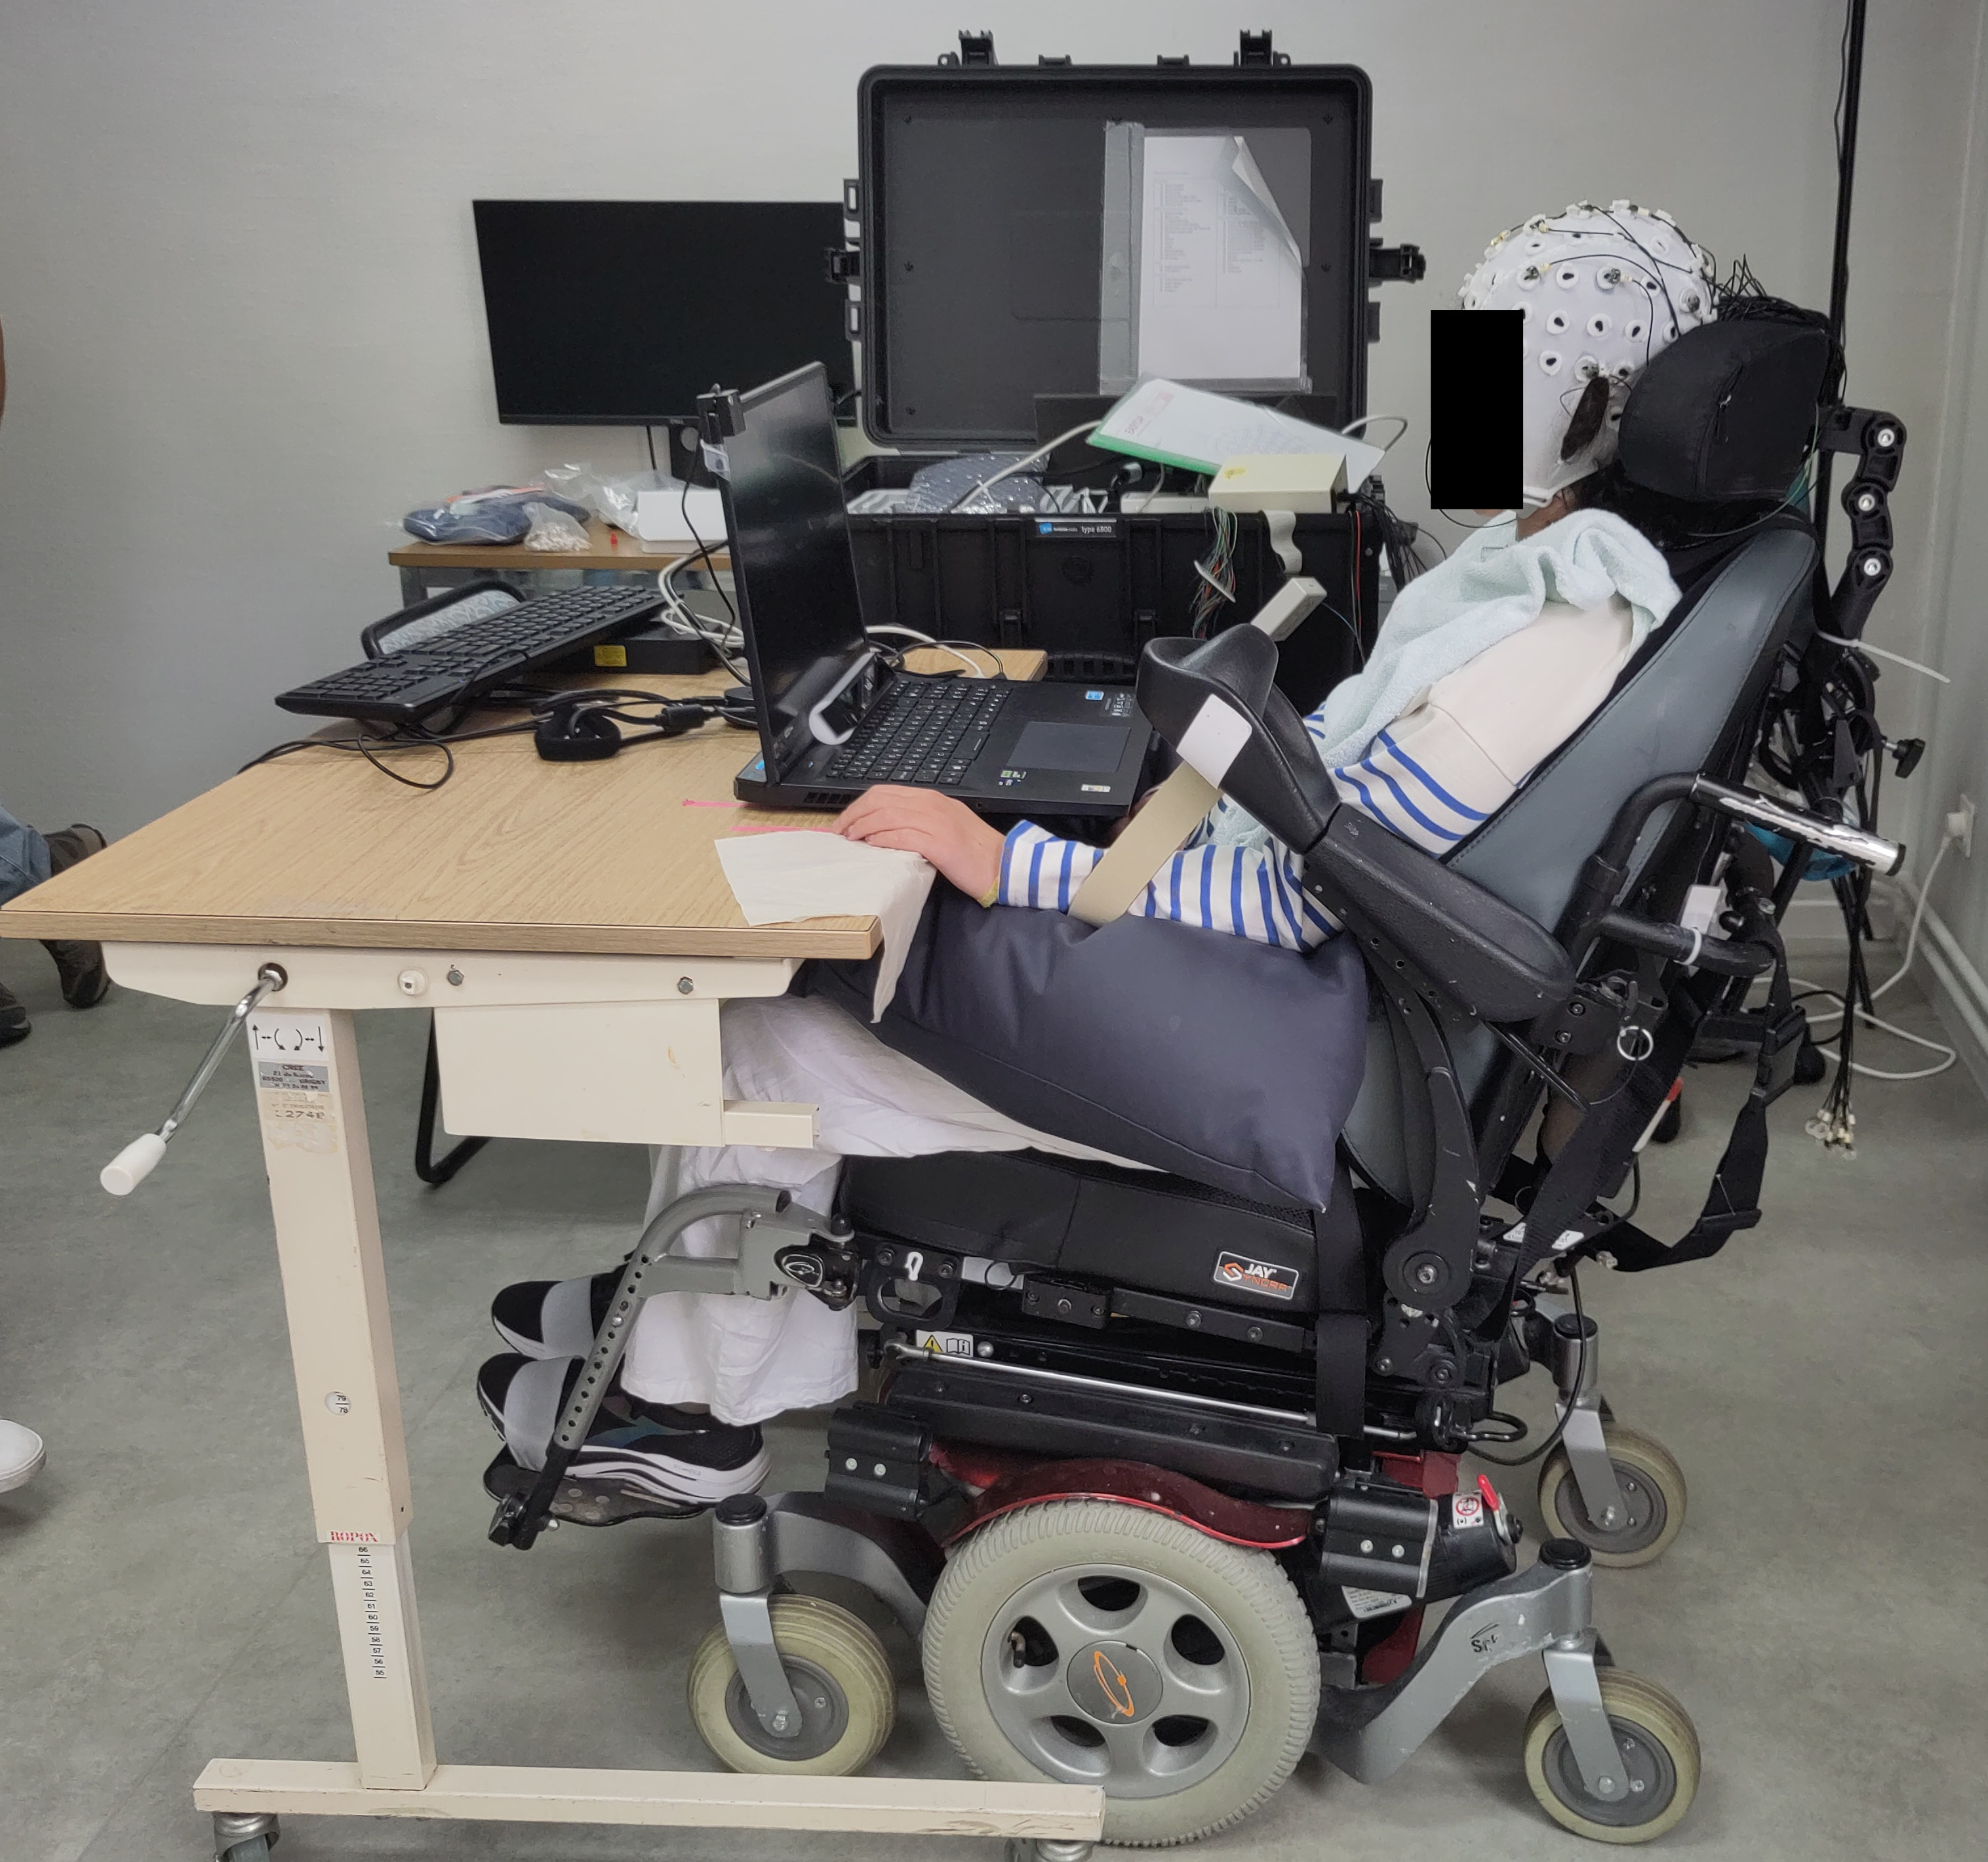
\includegraphics[width=\textwidth]{figures/patients/PD01a-obfuscated.jpg}}{A
  patient with the stimulation and recording setup.}{fig:patients/photos/side}
}{%
  \figpane{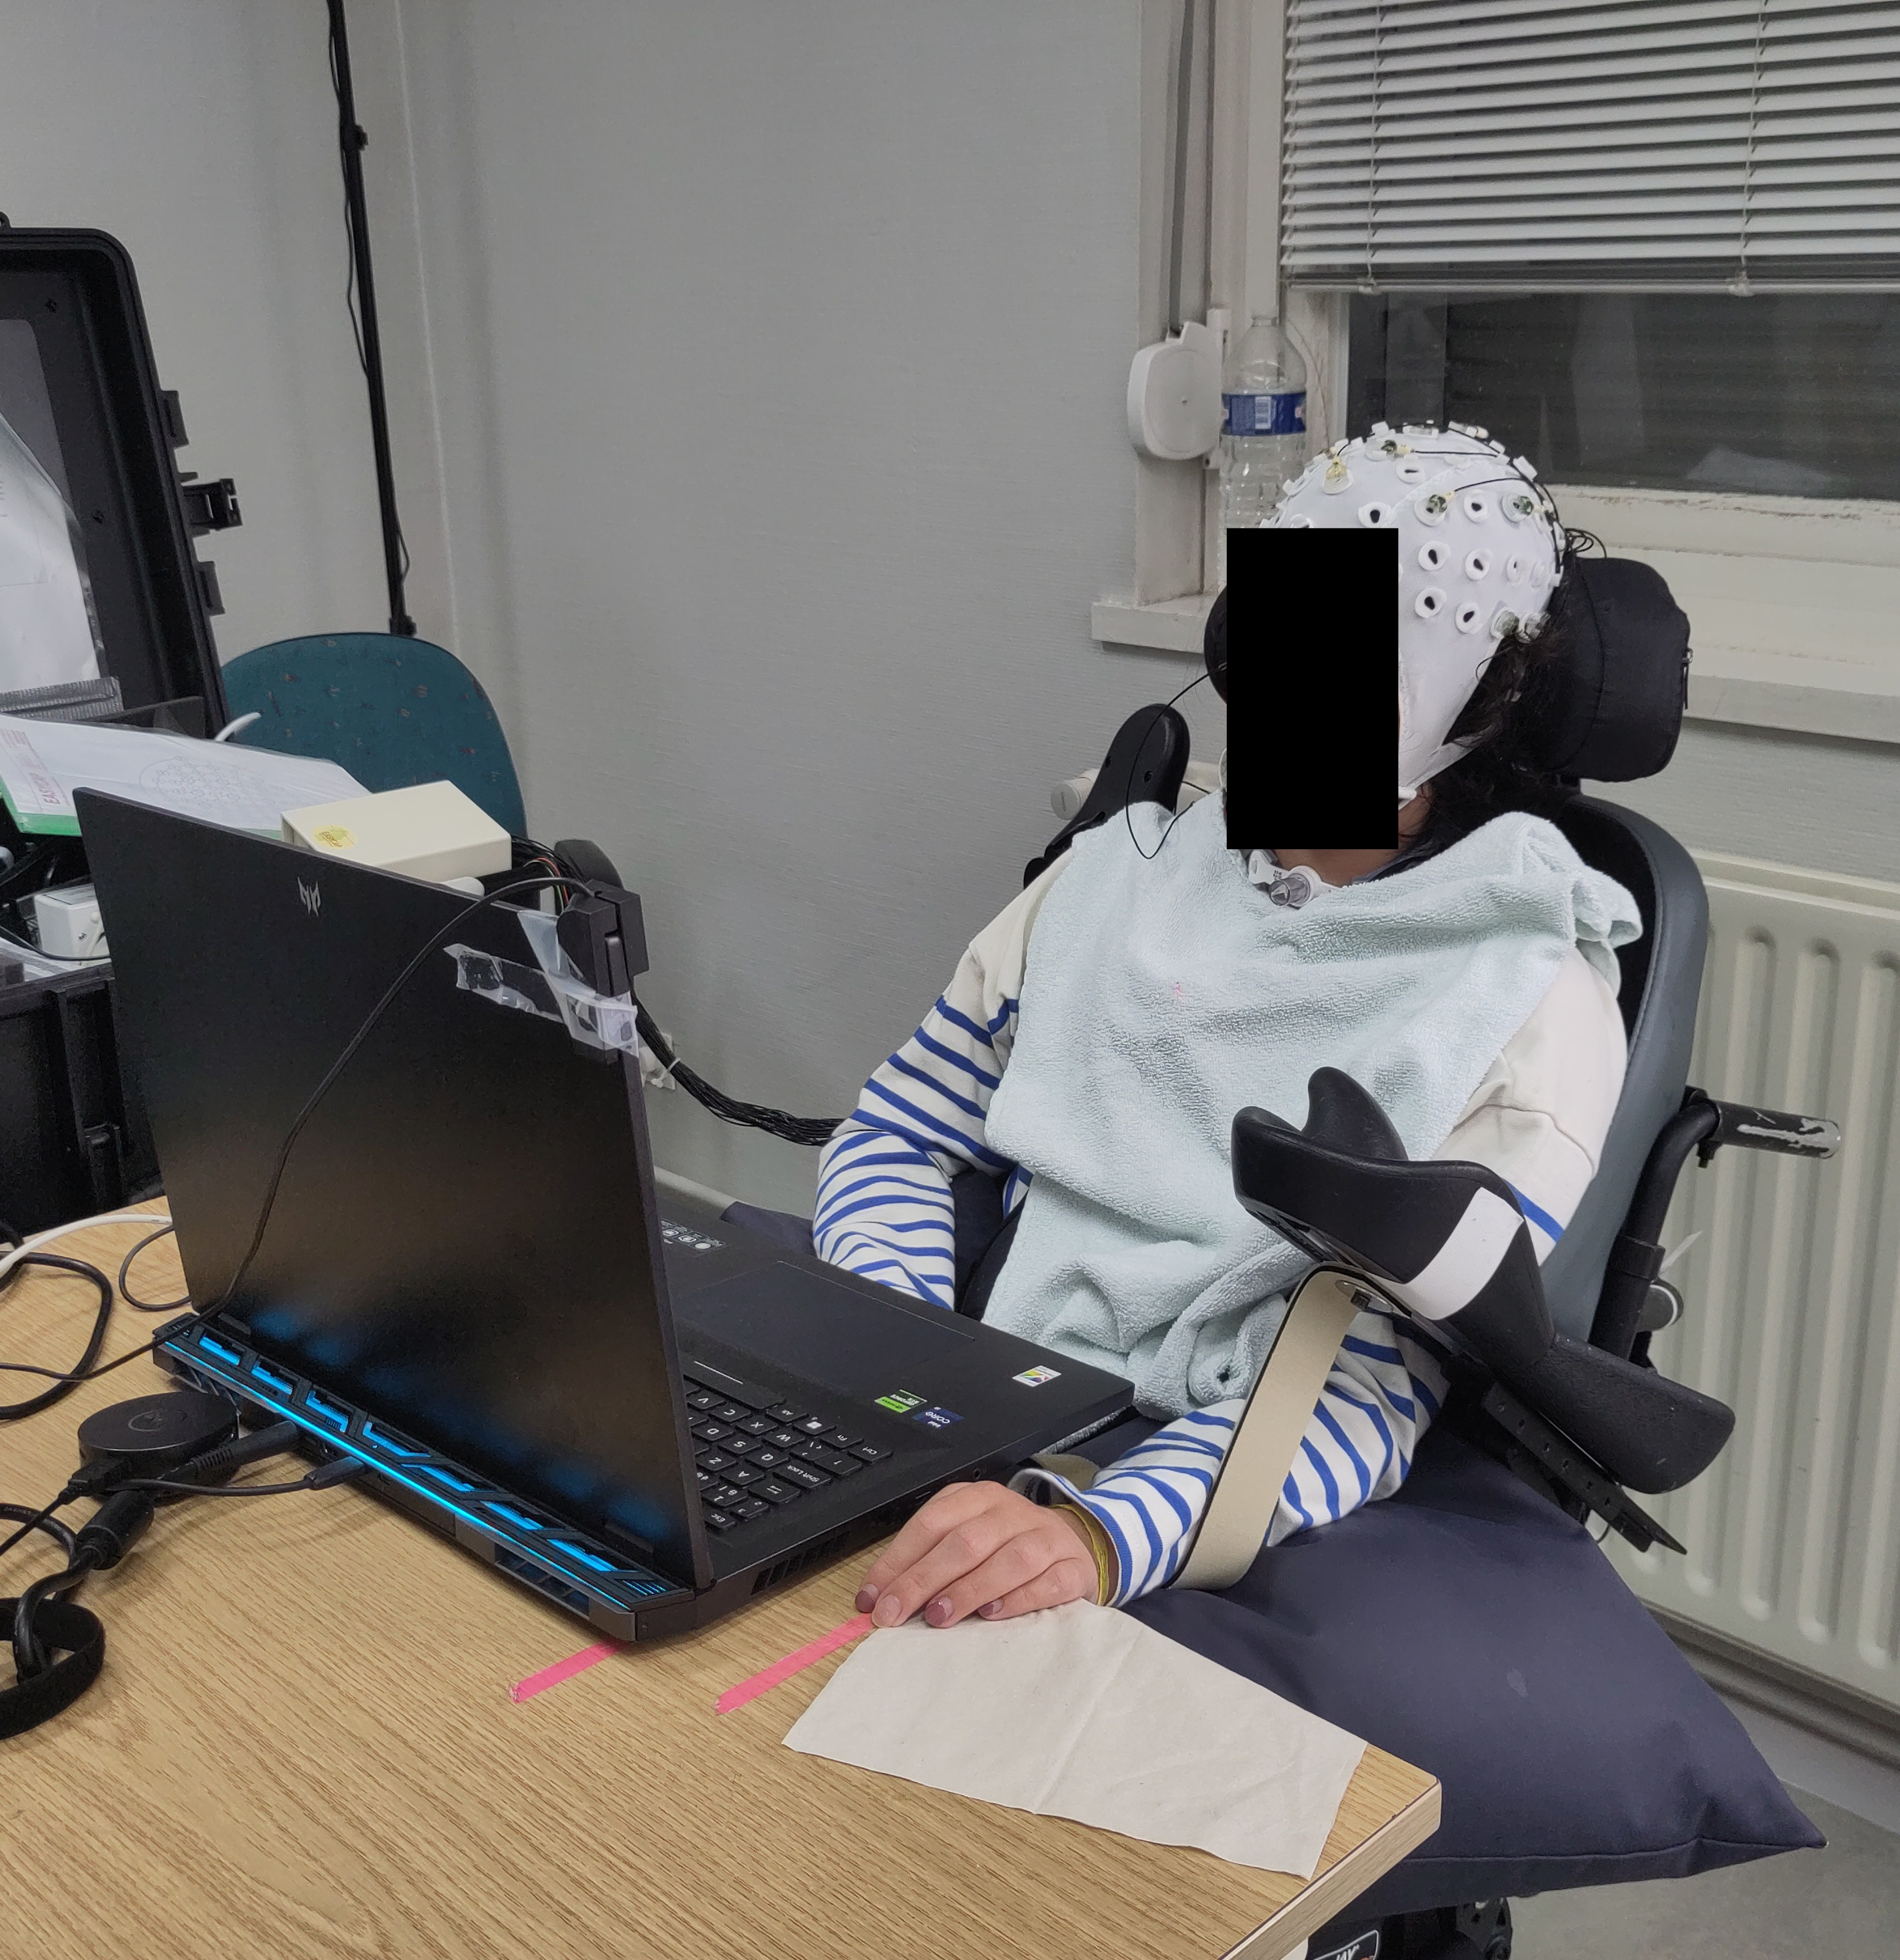
\includegraphics[width=\textwidth]{figures/patients/PD01b-obfuscated.jpg}}{subcaption}{fig:patients/photos/front}
}{%
  the interface
}{%
  4
}{%
  caption
}{fig:patients/photos}

Mention change in ISI
Mention less rounds

\subsection{Data collection \& preprocessing}

\todo{check checklist}
\subsection{BCI Decoding}

\section{Outcomes}

\subsection{Eye tracking analysis}

PC2 reported that he was unable to fixate the lower two targets, and th

\fullpagefig{%
  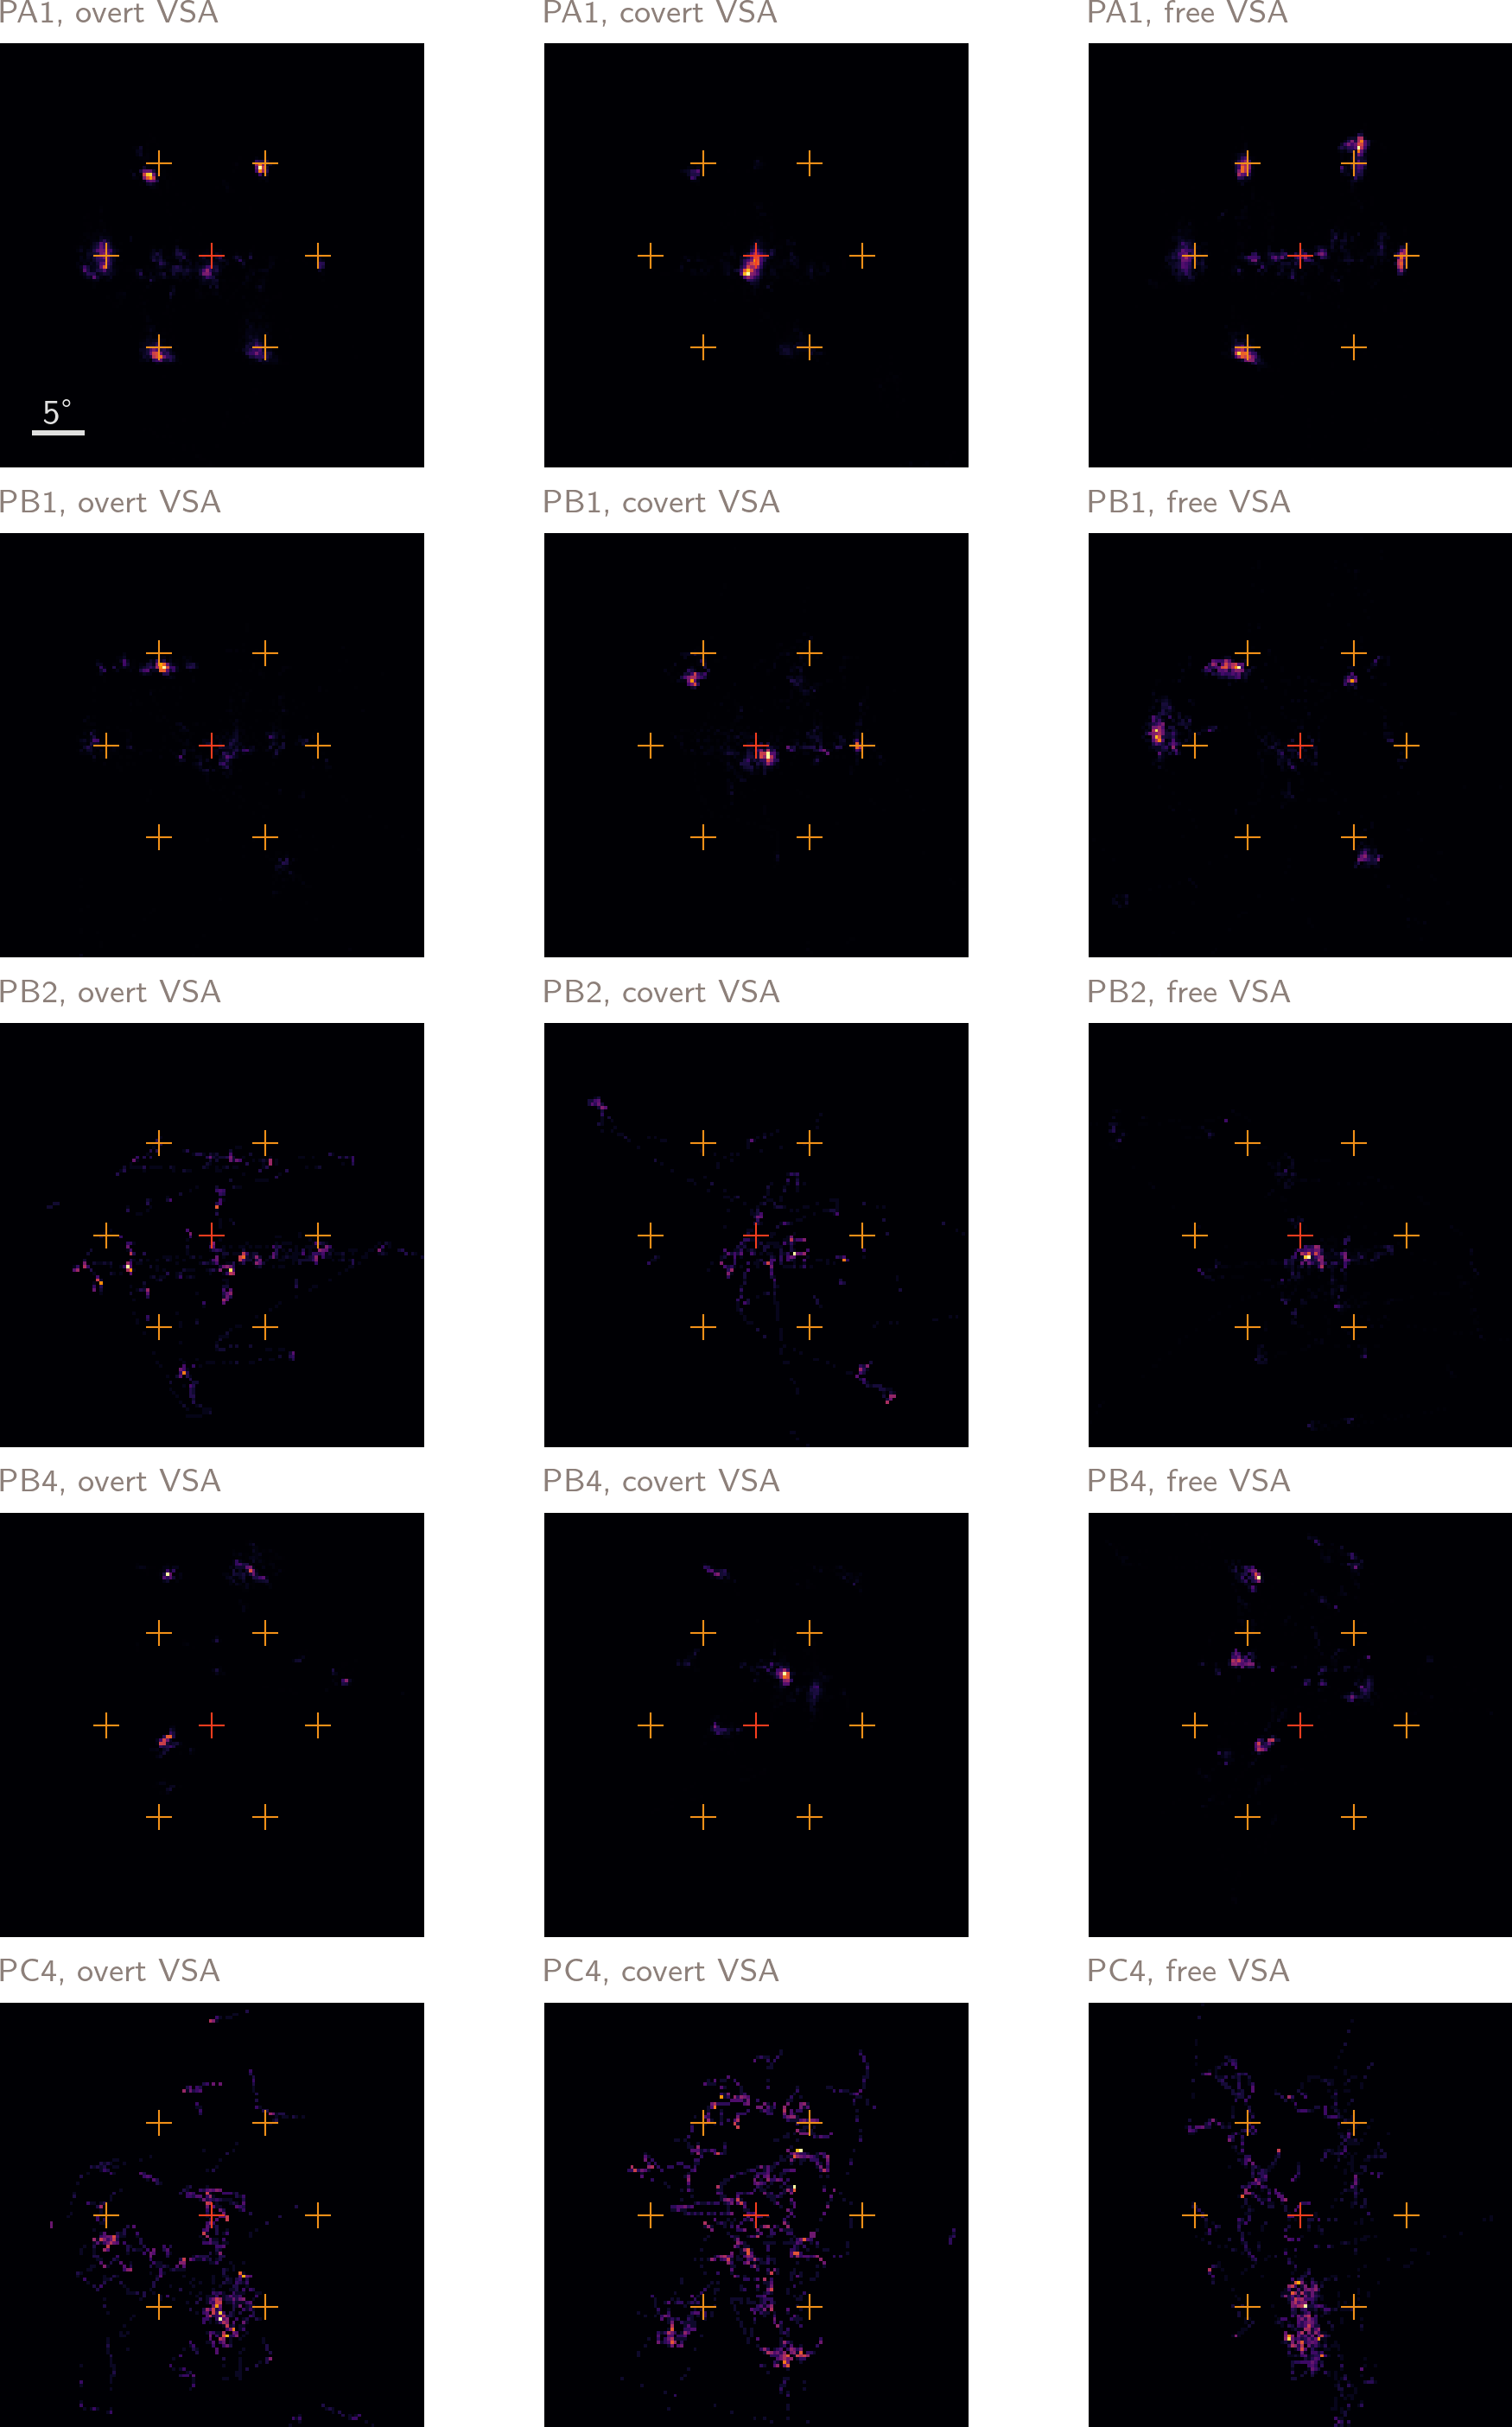
\includegraphics[width=\textwidth]{figures/patients/fig_gaze.png}
}{%
  Distribution of the recorded gaze position during the experimental session in the three \ac{vsa}
  conditions.
  Subjects PB2 and PC4 preferred covert \ac{bci} operation, with PB2 resting gaze
  near the middle of the screen, and PC4 near the bottom.
}{%
  fig:patients/gaze
}


\subsection{Decoding performance}

\begin{figure}[t]
  \hspace{-0.16816613518892673in}
%% Creator: Matplotlib, PGF backend
%%
%% To include the figure in your LaTeX document, write
%%   \input{<filename>.pgf}
%%
%% Make sure the required packages are loaded in your preamble
%%   \usepackage{pgf}
%%
%% Also ensure that all the required font packages are loaded; for instance,
%% the lmodern package is sometimes necessary when using math font.
%%   \usepackage{lmodern}
%%
%% Figures using additional raster images can only be included by \input if
%% they are in the same directory as the main LaTeX file. For loading figures
%% from other directories you can use the `import` package
%%   \usepackage{import}
%%
%% and then include the figures with
%%   \import{<path to file>}{<filename>.pgf}
%%
%% Matplotlib used the following preamble
%%
\begingroup%
\makeatletter%
\begin{pgfpicture}%
\pgfpathrectangle{\pgfpointorigin}{\pgfqpoint{4.941931in}{2.000000in}}%
\pgfusepath{use as bounding box, clip}%
\begin{pgfscope}%
\pgfsetbuttcap%
\pgfsetmiterjoin%
\definecolor{currentfill}{rgb}{1.000000,1.000000,1.000000}%
\pgfsetfillcolor{currentfill}%
\pgfsetlinewidth{0.000000pt}%
\definecolor{currentstroke}{rgb}{1.000000,1.000000,1.000000}%
\pgfsetstrokecolor{currentstroke}%
\pgfsetdash{}{0pt}%
\pgfpathmoveto{\pgfqpoint{0.000000in}{0.000000in}}%
\pgfpathlineto{\pgfqpoint{4.941931in}{0.000000in}}%
\pgfpathlineto{\pgfqpoint{4.941931in}{2.000000in}}%
\pgfpathlineto{\pgfqpoint{0.000000in}{2.000000in}}%
\pgfpathlineto{\pgfqpoint{0.000000in}{0.000000in}}%
\pgfpathclose%
\pgfusepath{fill}%
\end{pgfscope}%
\begin{pgfscope}%
\pgfsetbuttcap%
\pgfsetmiterjoin%
\definecolor{currentfill}{rgb}{1.000000,1.000000,1.000000}%
\pgfsetfillcolor{currentfill}%
\pgfsetlinewidth{0.000000pt}%
\definecolor{currentstroke}{rgb}{0.000000,0.000000,0.000000}%
\pgfsetstrokecolor{currentstroke}%
\pgfsetstrokeopacity{0.000000}%
\pgfsetdash{}{0pt}%
\pgfpathmoveto{\pgfqpoint{0.174090in}{0.190223in}}%
\pgfpathlineto{\pgfqpoint{1.713951in}{0.190223in}}%
\pgfpathlineto{\pgfqpoint{1.713951in}{1.872074in}}%
\pgfpathlineto{\pgfqpoint{0.174090in}{1.872074in}}%
\pgfpathlineto{\pgfqpoint{0.174090in}{0.190223in}}%
\pgfpathclose%
\pgfusepath{fill}%
\end{pgfscope}%
\begin{pgfscope}%
\pgfpathrectangle{\pgfqpoint{0.174090in}{0.190223in}}{\pgfqpoint{1.539861in}{1.681851in}}%
\pgfusepath{clip}%
\pgfsetbuttcap%
\pgfsetmiterjoin%
\definecolor{currentfill}{rgb}{0.842157,0.553922,0.200980}%
\pgfsetfillcolor{currentfill}%
\pgfsetlinewidth{0.000000pt}%
\definecolor{currentstroke}{rgb}{0.000000,0.000000,0.000000}%
\pgfsetstrokecolor{currentstroke}%
\pgfsetstrokeopacity{0.000000}%
\pgfsetdash{}{0pt}%
\pgfpathmoveto{\pgfqpoint{0.193338in}{0.190223in}}%
\pgfpathlineto{\pgfqpoint{0.244667in}{0.190223in}}%
\pgfpathlineto{\pgfqpoint{0.244667in}{1.317977in}}%
\pgfpathlineto{\pgfqpoint{0.193338in}{1.317977in}}%
\pgfpathlineto{\pgfqpoint{0.193338in}{0.190223in}}%
\pgfpathclose%
\pgfusepath{fill}%
\end{pgfscope}%
\begin{pgfscope}%
\pgfpathrectangle{\pgfqpoint{0.174090in}{0.190223in}}{\pgfqpoint{1.539861in}{1.681851in}}%
\pgfusepath{clip}%
\pgfsetbuttcap%
\pgfsetmiterjoin%
\definecolor{currentfill}{rgb}{0.842157,0.553922,0.200980}%
\pgfsetfillcolor{currentfill}%
\pgfsetlinewidth{0.000000pt}%
\definecolor{currentstroke}{rgb}{0.000000,0.000000,0.000000}%
\pgfsetstrokecolor{currentstroke}%
\pgfsetstrokeopacity{0.000000}%
\pgfsetdash{}{0pt}%
\pgfpathmoveto{\pgfqpoint{0.385821in}{0.190223in}}%
\pgfpathlineto{\pgfqpoint{0.437150in}{0.190223in}}%
\pgfpathlineto{\pgfqpoint{0.437150in}{1.717496in}}%
\pgfpathlineto{\pgfqpoint{0.385821in}{1.717496in}}%
\pgfpathlineto{\pgfqpoint{0.385821in}{0.190223in}}%
\pgfpathclose%
\pgfusepath{fill}%
\end{pgfscope}%
\begin{pgfscope}%
\pgfpathrectangle{\pgfqpoint{0.174090in}{0.190223in}}{\pgfqpoint{1.539861in}{1.681851in}}%
\pgfusepath{clip}%
\pgfsetbuttcap%
\pgfsetmiterjoin%
\definecolor{currentfill}{rgb}{0.842157,0.553922,0.200980}%
\pgfsetfillcolor{currentfill}%
\pgfsetlinewidth{0.000000pt}%
\definecolor{currentstroke}{rgb}{0.000000,0.000000,0.000000}%
\pgfsetstrokecolor{currentstroke}%
\pgfsetstrokeopacity{0.000000}%
\pgfsetdash{}{0pt}%
\pgfpathmoveto{\pgfqpoint{0.578304in}{0.190223in}}%
\pgfpathlineto{\pgfqpoint{0.629632in}{0.190223in}}%
\pgfpathlineto{\pgfqpoint{0.629632in}{1.589719in}}%
\pgfpathlineto{\pgfqpoint{0.578304in}{1.589719in}}%
\pgfpathlineto{\pgfqpoint{0.578304in}{0.190223in}}%
\pgfpathclose%
\pgfusepath{fill}%
\end{pgfscope}%
\begin{pgfscope}%
\pgfpathrectangle{\pgfqpoint{0.174090in}{0.190223in}}{\pgfqpoint{1.539861in}{1.681851in}}%
\pgfusepath{clip}%
\pgfsetbuttcap%
\pgfsetmiterjoin%
\definecolor{currentfill}{rgb}{0.842157,0.553922,0.200980}%
\pgfsetfillcolor{currentfill}%
\pgfsetlinewidth{0.000000pt}%
\definecolor{currentstroke}{rgb}{0.000000,0.000000,0.000000}%
\pgfsetstrokecolor{currentstroke}%
\pgfsetstrokeopacity{0.000000}%
\pgfsetdash{}{0pt}%
\pgfpathmoveto{\pgfqpoint{0.770786in}{0.190223in}}%
\pgfpathlineto{\pgfqpoint{0.822115in}{0.190223in}}%
\pgfpathlineto{\pgfqpoint{0.822115in}{1.589345in}}%
\pgfpathlineto{\pgfqpoint{0.770786in}{1.589345in}}%
\pgfpathlineto{\pgfqpoint{0.770786in}{0.190223in}}%
\pgfpathclose%
\pgfusepath{fill}%
\end{pgfscope}%
\begin{pgfscope}%
\pgfpathrectangle{\pgfqpoint{0.174090in}{0.190223in}}{\pgfqpoint{1.539861in}{1.681851in}}%
\pgfusepath{clip}%
\pgfsetbuttcap%
\pgfsetmiterjoin%
\definecolor{currentfill}{rgb}{0.842157,0.553922,0.200980}%
\pgfsetfillcolor{currentfill}%
\pgfsetlinewidth{0.000000pt}%
\definecolor{currentstroke}{rgb}{0.000000,0.000000,0.000000}%
\pgfsetstrokecolor{currentstroke}%
\pgfsetstrokeopacity{0.000000}%
\pgfsetdash{}{0pt}%
\pgfpathmoveto{\pgfqpoint{0.963269in}{0.190223in}}%
\pgfpathlineto{\pgfqpoint{1.014598in}{0.190223in}}%
\pgfpathlineto{\pgfqpoint{1.014598in}{1.384946in}}%
\pgfpathlineto{\pgfqpoint{0.963269in}{1.384946in}}%
\pgfpathlineto{\pgfqpoint{0.963269in}{0.190223in}}%
\pgfpathclose%
\pgfusepath{fill}%
\end{pgfscope}%
\begin{pgfscope}%
\pgfpathrectangle{\pgfqpoint{0.174090in}{0.190223in}}{\pgfqpoint{1.539861in}{1.681851in}}%
\pgfusepath{clip}%
\pgfsetbuttcap%
\pgfsetmiterjoin%
\definecolor{currentfill}{rgb}{0.842157,0.553922,0.200980}%
\pgfsetfillcolor{currentfill}%
\pgfsetlinewidth{0.000000pt}%
\definecolor{currentstroke}{rgb}{0.000000,0.000000,0.000000}%
\pgfsetstrokecolor{currentstroke}%
\pgfsetstrokeopacity{0.000000}%
\pgfsetdash{}{0pt}%
\pgfpathmoveto{\pgfqpoint{1.155752in}{0.190223in}}%
\pgfpathlineto{\pgfqpoint{1.207080in}{0.190223in}}%
\pgfpathlineto{\pgfqpoint{1.207080in}{1.375840in}}%
\pgfpathlineto{\pgfqpoint{1.155752in}{1.375840in}}%
\pgfpathlineto{\pgfqpoint{1.155752in}{0.190223in}}%
\pgfpathclose%
\pgfusepath{fill}%
\end{pgfscope}%
\begin{pgfscope}%
\pgfpathrectangle{\pgfqpoint{0.174090in}{0.190223in}}{\pgfqpoint{1.539861in}{1.681851in}}%
\pgfusepath{clip}%
\pgfsetbuttcap%
\pgfsetmiterjoin%
\definecolor{currentfill}{rgb}{0.842157,0.553922,0.200980}%
\pgfsetfillcolor{currentfill}%
\pgfsetlinewidth{0.000000pt}%
\definecolor{currentstroke}{rgb}{0.000000,0.000000,0.000000}%
\pgfsetstrokecolor{currentstroke}%
\pgfsetstrokeopacity{0.000000}%
\pgfsetdash{}{0pt}%
\pgfpathmoveto{\pgfqpoint{1.348234in}{0.190223in}}%
\pgfpathlineto{\pgfqpoint{1.399563in}{0.190223in}}%
\pgfpathlineto{\pgfqpoint{1.399563in}{1.302232in}}%
\pgfpathlineto{\pgfqpoint{1.348234in}{1.302232in}}%
\pgfpathlineto{\pgfqpoint{1.348234in}{0.190223in}}%
\pgfpathclose%
\pgfusepath{fill}%
\end{pgfscope}%
\begin{pgfscope}%
\pgfpathrectangle{\pgfqpoint{0.174090in}{0.190223in}}{\pgfqpoint{1.539861in}{1.681851in}}%
\pgfusepath{clip}%
\pgfsetbuttcap%
\pgfsetmiterjoin%
\definecolor{currentfill}{rgb}{0.842157,0.553922,0.200980}%
\pgfsetfillcolor{currentfill}%
\pgfsetlinewidth{0.000000pt}%
\definecolor{currentstroke}{rgb}{0.000000,0.000000,0.000000}%
\pgfsetstrokecolor{currentstroke}%
\pgfsetstrokeopacity{0.000000}%
\pgfsetdash{}{0pt}%
\pgfpathmoveto{\pgfqpoint{1.540717in}{0.190223in}}%
\pgfpathlineto{\pgfqpoint{1.592046in}{0.190223in}}%
\pgfpathlineto{\pgfqpoint{1.592046in}{1.468222in}}%
\pgfpathlineto{\pgfqpoint{1.540717in}{1.468222in}}%
\pgfpathlineto{\pgfqpoint{1.540717in}{0.190223in}}%
\pgfpathclose%
\pgfusepath{fill}%
\end{pgfscope}%
\begin{pgfscope}%
\pgfpathrectangle{\pgfqpoint{0.174090in}{0.190223in}}{\pgfqpoint{1.539861in}{1.681851in}}%
\pgfusepath{clip}%
\pgfsetbuttcap%
\pgfsetmiterjoin%
\definecolor{currentfill}{rgb}{0.858824,0.314706,0.223529}%
\pgfsetfillcolor{currentfill}%
\pgfsetlinewidth{0.000000pt}%
\definecolor{currentstroke}{rgb}{0.000000,0.000000,0.000000}%
\pgfsetstrokecolor{currentstroke}%
\pgfsetstrokeopacity{0.000000}%
\pgfsetdash{}{0pt}%
\pgfpathmoveto{\pgfqpoint{0.244667in}{0.190223in}}%
\pgfpathlineto{\pgfqpoint{0.295996in}{0.190223in}}%
\pgfpathlineto{\pgfqpoint{0.295996in}{1.393596in}}%
\pgfpathlineto{\pgfqpoint{0.244667in}{1.393596in}}%
\pgfpathlineto{\pgfqpoint{0.244667in}{0.190223in}}%
\pgfpathclose%
\pgfusepath{fill}%
\end{pgfscope}%
\begin{pgfscope}%
\pgfpathrectangle{\pgfqpoint{0.174090in}{0.190223in}}{\pgfqpoint{1.539861in}{1.681851in}}%
\pgfusepath{clip}%
\pgfsetbuttcap%
\pgfsetmiterjoin%
\definecolor{currentfill}{rgb}{0.858824,0.314706,0.223529}%
\pgfsetfillcolor{currentfill}%
\pgfsetlinewidth{0.000000pt}%
\definecolor{currentstroke}{rgb}{0.000000,0.000000,0.000000}%
\pgfsetstrokecolor{currentstroke}%
\pgfsetstrokeopacity{0.000000}%
\pgfsetdash{}{0pt}%
\pgfpathmoveto{\pgfqpoint{0.437150in}{0.190223in}}%
\pgfpathlineto{\pgfqpoint{0.488478in}{0.190223in}}%
\pgfpathlineto{\pgfqpoint{0.488478in}{1.695290in}}%
\pgfpathlineto{\pgfqpoint{0.437150in}{1.695290in}}%
\pgfpathlineto{\pgfqpoint{0.437150in}{0.190223in}}%
\pgfpathclose%
\pgfusepath{fill}%
\end{pgfscope}%
\begin{pgfscope}%
\pgfpathrectangle{\pgfqpoint{0.174090in}{0.190223in}}{\pgfqpoint{1.539861in}{1.681851in}}%
\pgfusepath{clip}%
\pgfsetbuttcap%
\pgfsetmiterjoin%
\definecolor{currentfill}{rgb}{0.858824,0.314706,0.223529}%
\pgfsetfillcolor{currentfill}%
\pgfsetlinewidth{0.000000pt}%
\definecolor{currentstroke}{rgb}{0.000000,0.000000,0.000000}%
\pgfsetstrokecolor{currentstroke}%
\pgfsetstrokeopacity{0.000000}%
\pgfsetdash{}{0pt}%
\pgfpathmoveto{\pgfqpoint{0.629632in}{0.190223in}}%
\pgfpathlineto{\pgfqpoint{0.680961in}{0.190223in}}%
\pgfpathlineto{\pgfqpoint{0.680961in}{1.582085in}}%
\pgfpathlineto{\pgfqpoint{0.629632in}{1.582085in}}%
\pgfpathlineto{\pgfqpoint{0.629632in}{0.190223in}}%
\pgfpathclose%
\pgfusepath{fill}%
\end{pgfscope}%
\begin{pgfscope}%
\pgfpathrectangle{\pgfqpoint{0.174090in}{0.190223in}}{\pgfqpoint{1.539861in}{1.681851in}}%
\pgfusepath{clip}%
\pgfsetbuttcap%
\pgfsetmiterjoin%
\definecolor{currentfill}{rgb}{0.858824,0.314706,0.223529}%
\pgfsetfillcolor{currentfill}%
\pgfsetlinewidth{0.000000pt}%
\definecolor{currentstroke}{rgb}{0.000000,0.000000,0.000000}%
\pgfsetstrokecolor{currentstroke}%
\pgfsetstrokeopacity{0.000000}%
\pgfsetdash{}{0pt}%
\pgfpathmoveto{\pgfqpoint{0.822115in}{0.190223in}}%
\pgfpathlineto{\pgfqpoint{0.873444in}{0.190223in}}%
\pgfpathlineto{\pgfqpoint{0.873444in}{1.544680in}}%
\pgfpathlineto{\pgfqpoint{0.822115in}{1.544680in}}%
\pgfpathlineto{\pgfqpoint{0.822115in}{0.190223in}}%
\pgfpathclose%
\pgfusepath{fill}%
\end{pgfscope}%
\begin{pgfscope}%
\pgfpathrectangle{\pgfqpoint{0.174090in}{0.190223in}}{\pgfqpoint{1.539861in}{1.681851in}}%
\pgfusepath{clip}%
\pgfsetbuttcap%
\pgfsetmiterjoin%
\definecolor{currentfill}{rgb}{0.858824,0.314706,0.223529}%
\pgfsetfillcolor{currentfill}%
\pgfsetlinewidth{0.000000pt}%
\definecolor{currentstroke}{rgb}{0.000000,0.000000,0.000000}%
\pgfsetstrokecolor{currentstroke}%
\pgfsetstrokeopacity{0.000000}%
\pgfsetdash{}{0pt}%
\pgfpathmoveto{\pgfqpoint{1.014598in}{0.190223in}}%
\pgfpathlineto{\pgfqpoint{1.065926in}{0.190223in}}%
\pgfpathlineto{\pgfqpoint{1.065926in}{1.346833in}}%
\pgfpathlineto{\pgfqpoint{1.014598in}{1.346833in}}%
\pgfpathlineto{\pgfqpoint{1.014598in}{0.190223in}}%
\pgfpathclose%
\pgfusepath{fill}%
\end{pgfscope}%
\begin{pgfscope}%
\pgfpathrectangle{\pgfqpoint{0.174090in}{0.190223in}}{\pgfqpoint{1.539861in}{1.681851in}}%
\pgfusepath{clip}%
\pgfsetbuttcap%
\pgfsetmiterjoin%
\definecolor{currentfill}{rgb}{0.858824,0.314706,0.223529}%
\pgfsetfillcolor{currentfill}%
\pgfsetlinewidth{0.000000pt}%
\definecolor{currentstroke}{rgb}{0.000000,0.000000,0.000000}%
\pgfsetstrokecolor{currentstroke}%
\pgfsetstrokeopacity{0.000000}%
\pgfsetdash{}{0pt}%
\pgfpathmoveto{\pgfqpoint{1.207080in}{0.190223in}}%
\pgfpathlineto{\pgfqpoint{1.258409in}{0.190223in}}%
\pgfpathlineto{\pgfqpoint{1.258409in}{1.372747in}}%
\pgfpathlineto{\pgfqpoint{1.207080in}{1.372747in}}%
\pgfpathlineto{\pgfqpoint{1.207080in}{0.190223in}}%
\pgfpathclose%
\pgfusepath{fill}%
\end{pgfscope}%
\begin{pgfscope}%
\pgfpathrectangle{\pgfqpoint{0.174090in}{0.190223in}}{\pgfqpoint{1.539861in}{1.681851in}}%
\pgfusepath{clip}%
\pgfsetbuttcap%
\pgfsetmiterjoin%
\definecolor{currentfill}{rgb}{0.858824,0.314706,0.223529}%
\pgfsetfillcolor{currentfill}%
\pgfsetlinewidth{0.000000pt}%
\definecolor{currentstroke}{rgb}{0.000000,0.000000,0.000000}%
\pgfsetstrokecolor{currentstroke}%
\pgfsetstrokeopacity{0.000000}%
\pgfsetdash{}{0pt}%
\pgfpathmoveto{\pgfqpoint{1.399563in}{0.190223in}}%
\pgfpathlineto{\pgfqpoint{1.450892in}{0.190223in}}%
\pgfpathlineto{\pgfqpoint{1.450892in}{1.294360in}}%
\pgfpathlineto{\pgfqpoint{1.399563in}{1.294360in}}%
\pgfpathlineto{\pgfqpoint{1.399563in}{0.190223in}}%
\pgfpathclose%
\pgfusepath{fill}%
\end{pgfscope}%
\begin{pgfscope}%
\pgfpathrectangle{\pgfqpoint{0.174090in}{0.190223in}}{\pgfqpoint{1.539861in}{1.681851in}}%
\pgfusepath{clip}%
\pgfsetbuttcap%
\pgfsetmiterjoin%
\definecolor{currentfill}{rgb}{0.858824,0.314706,0.223529}%
\pgfsetfillcolor{currentfill}%
\pgfsetlinewidth{0.000000pt}%
\definecolor{currentstroke}{rgb}{0.000000,0.000000,0.000000}%
\pgfsetstrokecolor{currentstroke}%
\pgfsetstrokeopacity{0.000000}%
\pgfsetdash{}{0pt}%
\pgfpathmoveto{\pgfqpoint{1.592046in}{0.190223in}}%
\pgfpathlineto{\pgfqpoint{1.643374in}{0.190223in}}%
\pgfpathlineto{\pgfqpoint{1.643374in}{1.461370in}}%
\pgfpathlineto{\pgfqpoint{1.592046in}{1.461370in}}%
\pgfpathlineto{\pgfqpoint{1.592046in}{0.190223in}}%
\pgfpathclose%
\pgfusepath{fill}%
\end{pgfscope}%
\begin{pgfscope}%
\pgfpathrectangle{\pgfqpoint{0.174090in}{0.190223in}}{\pgfqpoint{1.539861in}{1.681851in}}%
\pgfusepath{clip}%
\pgfsetbuttcap%
\pgfsetmiterjoin%
\definecolor{currentfill}{rgb}{0.464706,0.320588,0.573529}%
\pgfsetfillcolor{currentfill}%
\pgfsetlinewidth{0.000000pt}%
\definecolor{currentstroke}{rgb}{0.000000,0.000000,0.000000}%
\pgfsetstrokecolor{currentstroke}%
\pgfsetstrokeopacity{0.000000}%
\pgfsetdash{}{0pt}%
\pgfpathmoveto{\pgfqpoint{0.295996in}{0.190223in}}%
\pgfpathlineto{\pgfqpoint{0.347325in}{0.190223in}}%
\pgfpathlineto{\pgfqpoint{0.347325in}{1.332130in}}%
\pgfpathlineto{\pgfqpoint{0.295996in}{1.332130in}}%
\pgfpathlineto{\pgfqpoint{0.295996in}{0.190223in}}%
\pgfpathclose%
\pgfusepath{fill}%
\end{pgfscope}%
\begin{pgfscope}%
\pgfpathrectangle{\pgfqpoint{0.174090in}{0.190223in}}{\pgfqpoint{1.539861in}{1.681851in}}%
\pgfusepath{clip}%
\pgfsetbuttcap%
\pgfsetmiterjoin%
\definecolor{currentfill}{rgb}{0.464706,0.320588,0.573529}%
\pgfsetfillcolor{currentfill}%
\pgfsetlinewidth{0.000000pt}%
\definecolor{currentstroke}{rgb}{0.000000,0.000000,0.000000}%
\pgfsetstrokecolor{currentstroke}%
\pgfsetstrokeopacity{0.000000}%
\pgfsetdash{}{0pt}%
\pgfpathmoveto{\pgfqpoint{0.488478in}{0.190223in}}%
\pgfpathlineto{\pgfqpoint{0.539807in}{0.190223in}}%
\pgfpathlineto{\pgfqpoint{0.539807in}{1.696667in}}%
\pgfpathlineto{\pgfqpoint{0.488478in}{1.696667in}}%
\pgfpathlineto{\pgfqpoint{0.488478in}{0.190223in}}%
\pgfpathclose%
\pgfusepath{fill}%
\end{pgfscope}%
\begin{pgfscope}%
\pgfpathrectangle{\pgfqpoint{0.174090in}{0.190223in}}{\pgfqpoint{1.539861in}{1.681851in}}%
\pgfusepath{clip}%
\pgfsetbuttcap%
\pgfsetmiterjoin%
\definecolor{currentfill}{rgb}{0.464706,0.320588,0.573529}%
\pgfsetfillcolor{currentfill}%
\pgfsetlinewidth{0.000000pt}%
\definecolor{currentstroke}{rgb}{0.000000,0.000000,0.000000}%
\pgfsetstrokecolor{currentstroke}%
\pgfsetstrokeopacity{0.000000}%
\pgfsetdash{}{0pt}%
\pgfpathmoveto{\pgfqpoint{0.680961in}{0.190223in}}%
\pgfpathlineto{\pgfqpoint{0.732290in}{0.190223in}}%
\pgfpathlineto{\pgfqpoint{0.732290in}{1.548223in}}%
\pgfpathlineto{\pgfqpoint{0.680961in}{1.548223in}}%
\pgfpathlineto{\pgfqpoint{0.680961in}{0.190223in}}%
\pgfpathclose%
\pgfusepath{fill}%
\end{pgfscope}%
\begin{pgfscope}%
\pgfpathrectangle{\pgfqpoint{0.174090in}{0.190223in}}{\pgfqpoint{1.539861in}{1.681851in}}%
\pgfusepath{clip}%
\pgfsetbuttcap%
\pgfsetmiterjoin%
\definecolor{currentfill}{rgb}{0.464706,0.320588,0.573529}%
\pgfsetfillcolor{currentfill}%
\pgfsetlinewidth{0.000000pt}%
\definecolor{currentstroke}{rgb}{0.000000,0.000000,0.000000}%
\pgfsetstrokecolor{currentstroke}%
\pgfsetstrokeopacity{0.000000}%
\pgfsetdash{}{0pt}%
\pgfpathmoveto{\pgfqpoint{0.873444in}{0.190223in}}%
\pgfpathlineto{\pgfqpoint{0.924772in}{0.190223in}}%
\pgfpathlineto{\pgfqpoint{0.924772in}{1.582413in}}%
\pgfpathlineto{\pgfqpoint{0.873444in}{1.582413in}}%
\pgfpathlineto{\pgfqpoint{0.873444in}{0.190223in}}%
\pgfpathclose%
\pgfusepath{fill}%
\end{pgfscope}%
\begin{pgfscope}%
\pgfpathrectangle{\pgfqpoint{0.174090in}{0.190223in}}{\pgfqpoint{1.539861in}{1.681851in}}%
\pgfusepath{clip}%
\pgfsetbuttcap%
\pgfsetmiterjoin%
\definecolor{currentfill}{rgb}{0.464706,0.320588,0.573529}%
\pgfsetfillcolor{currentfill}%
\pgfsetlinewidth{0.000000pt}%
\definecolor{currentstroke}{rgb}{0.000000,0.000000,0.000000}%
\pgfsetstrokecolor{currentstroke}%
\pgfsetstrokeopacity{0.000000}%
\pgfsetdash{}{0pt}%
\pgfpathmoveto{\pgfqpoint{1.065926in}{0.190223in}}%
\pgfpathlineto{\pgfqpoint{1.117255in}{0.190223in}}%
\pgfpathlineto{\pgfqpoint{1.117255in}{1.389045in}}%
\pgfpathlineto{\pgfqpoint{1.065926in}{1.389045in}}%
\pgfpathlineto{\pgfqpoint{1.065926in}{0.190223in}}%
\pgfpathclose%
\pgfusepath{fill}%
\end{pgfscope}%
\begin{pgfscope}%
\pgfpathrectangle{\pgfqpoint{0.174090in}{0.190223in}}{\pgfqpoint{1.539861in}{1.681851in}}%
\pgfusepath{clip}%
\pgfsetbuttcap%
\pgfsetmiterjoin%
\definecolor{currentfill}{rgb}{0.464706,0.320588,0.573529}%
\pgfsetfillcolor{currentfill}%
\pgfsetlinewidth{0.000000pt}%
\definecolor{currentstroke}{rgb}{0.000000,0.000000,0.000000}%
\pgfsetstrokecolor{currentstroke}%
\pgfsetstrokeopacity{0.000000}%
\pgfsetdash{}{0pt}%
\pgfpathmoveto{\pgfqpoint{1.258409in}{0.190223in}}%
\pgfpathlineto{\pgfqpoint{1.309738in}{0.190223in}}%
\pgfpathlineto{\pgfqpoint{1.309738in}{1.289552in}}%
\pgfpathlineto{\pgfqpoint{1.258409in}{1.289552in}}%
\pgfpathlineto{\pgfqpoint{1.258409in}{0.190223in}}%
\pgfpathclose%
\pgfusepath{fill}%
\end{pgfscope}%
\begin{pgfscope}%
\pgfpathrectangle{\pgfqpoint{0.174090in}{0.190223in}}{\pgfqpoint{1.539861in}{1.681851in}}%
\pgfusepath{clip}%
\pgfsetbuttcap%
\pgfsetmiterjoin%
\definecolor{currentfill}{rgb}{0.464706,0.320588,0.573529}%
\pgfsetfillcolor{currentfill}%
\pgfsetlinewidth{0.000000pt}%
\definecolor{currentstroke}{rgb}{0.000000,0.000000,0.000000}%
\pgfsetstrokecolor{currentstroke}%
\pgfsetstrokeopacity{0.000000}%
\pgfsetdash{}{0pt}%
\pgfpathmoveto{\pgfqpoint{1.450892in}{0.190223in}}%
\pgfpathlineto{\pgfqpoint{1.502220in}{0.190223in}}%
\pgfpathlineto{\pgfqpoint{1.502220in}{1.233230in}}%
\pgfpathlineto{\pgfqpoint{1.450892in}{1.233230in}}%
\pgfpathlineto{\pgfqpoint{1.450892in}{0.190223in}}%
\pgfpathclose%
\pgfusepath{fill}%
\end{pgfscope}%
\begin{pgfscope}%
\pgfpathrectangle{\pgfqpoint{0.174090in}{0.190223in}}{\pgfqpoint{1.539861in}{1.681851in}}%
\pgfusepath{clip}%
\pgfsetbuttcap%
\pgfsetmiterjoin%
\definecolor{currentfill}{rgb}{0.464706,0.320588,0.573529}%
\pgfsetfillcolor{currentfill}%
\pgfsetlinewidth{0.000000pt}%
\definecolor{currentstroke}{rgb}{0.000000,0.000000,0.000000}%
\pgfsetstrokecolor{currentstroke}%
\pgfsetstrokeopacity{0.000000}%
\pgfsetdash{}{0pt}%
\pgfpathmoveto{\pgfqpoint{1.643374in}{0.190223in}}%
\pgfpathlineto{\pgfqpoint{1.694703in}{0.190223in}}%
\pgfpathlineto{\pgfqpoint{1.694703in}{1.438751in}}%
\pgfpathlineto{\pgfqpoint{1.643374in}{1.438751in}}%
\pgfpathlineto{\pgfqpoint{1.643374in}{0.190223in}}%
\pgfpathclose%
\pgfusepath{fill}%
\end{pgfscope}%
\begin{pgfscope}%
\pgfsetbuttcap%
\pgfsetroundjoin%
\definecolor{currentfill}{rgb}{0.552941,0.501961,0.478431}%
\pgfsetfillcolor{currentfill}%
\pgfsetlinewidth{0.803000pt}%
\definecolor{currentstroke}{rgb}{0.552941,0.501961,0.478431}%
\pgfsetstrokecolor{currentstroke}%
\pgfsetdash{}{0pt}%
\pgfsys@defobject{currentmarker}{\pgfqpoint{0.000000in}{0.000000in}}{\pgfqpoint{0.000000in}{0.041667in}}{%
\pgfpathmoveto{\pgfqpoint{0.000000in}{0.000000in}}%
\pgfpathlineto{\pgfqpoint{0.000000in}{0.041667in}}%
\pgfusepath{stroke,fill}%
}%
\begin{pgfscope}%
\pgfsys@transformshift{0.270331in}{0.190223in}%
\pgfsys@useobject{currentmarker}{}%
\end{pgfscope}%
\end{pgfscope}%
\begin{pgfscope}%
\definecolor{textcolor}{rgb}{0.552941,0.501961,0.478431}%
\pgfsetstrokecolor{textcolor}%
\pgfsetfillcolor{textcolor}%
\pgftext[x=0.301581in, y=-0.079933in, left, base,rotate=90.000000]{\color{textcolor}\sffamily\fontsize{9.000000}{10.800000}\selectfont PA1}%
\end{pgfscope}%
\begin{pgfscope}%
\pgfsetbuttcap%
\pgfsetroundjoin%
\definecolor{currentfill}{rgb}{0.552941,0.501961,0.478431}%
\pgfsetfillcolor{currentfill}%
\pgfsetlinewidth{0.803000pt}%
\definecolor{currentstroke}{rgb}{0.552941,0.501961,0.478431}%
\pgfsetstrokecolor{currentstroke}%
\pgfsetdash{}{0pt}%
\pgfsys@defobject{currentmarker}{\pgfqpoint{0.000000in}{0.000000in}}{\pgfqpoint{0.000000in}{0.041667in}}{%
\pgfpathmoveto{\pgfqpoint{0.000000in}{0.000000in}}%
\pgfpathlineto{\pgfqpoint{0.000000in}{0.041667in}}%
\pgfusepath{stroke,fill}%
}%
\begin{pgfscope}%
\pgfsys@transformshift{0.462814in}{0.190223in}%
\pgfsys@useobject{currentmarker}{}%
\end{pgfscope}%
\end{pgfscope}%
\begin{pgfscope}%
\definecolor{textcolor}{rgb}{0.552941,0.501961,0.478431}%
\pgfsetstrokecolor{textcolor}%
\pgfsetfillcolor{textcolor}%
\pgftext[x=0.494064in, y=-0.090543in, left, base,rotate=90.000000]{\color{textcolor}\sffamily\fontsize{9.000000}{10.800000}\selectfont PB1}%
\end{pgfscope}%
\begin{pgfscope}%
\pgfsetbuttcap%
\pgfsetroundjoin%
\definecolor{currentfill}{rgb}{0.552941,0.501961,0.478431}%
\pgfsetfillcolor{currentfill}%
\pgfsetlinewidth{0.803000pt}%
\definecolor{currentstroke}{rgb}{0.552941,0.501961,0.478431}%
\pgfsetstrokecolor{currentstroke}%
\pgfsetdash{}{0pt}%
\pgfsys@defobject{currentmarker}{\pgfqpoint{0.000000in}{0.000000in}}{\pgfqpoint{0.000000in}{0.041667in}}{%
\pgfpathmoveto{\pgfqpoint{0.000000in}{0.000000in}}%
\pgfpathlineto{\pgfqpoint{0.000000in}{0.041667in}}%
\pgfusepath{stroke,fill}%
}%
\begin{pgfscope}%
\pgfsys@transformshift{0.655297in}{0.190223in}%
\pgfsys@useobject{currentmarker}{}%
\end{pgfscope}%
\end{pgfscope}%
\begin{pgfscope}%
\definecolor{textcolor}{rgb}{0.552941,0.501961,0.478431}%
\pgfsetstrokecolor{textcolor}%
\pgfsetfillcolor{textcolor}%
\pgftext[x=0.686547in, y=-0.090543in, left, base,rotate=90.000000]{\color{textcolor}\sffamily\fontsize{9.000000}{10.800000}\selectfont PB2}%
\end{pgfscope}%
\begin{pgfscope}%
\pgfsetbuttcap%
\pgfsetroundjoin%
\definecolor{currentfill}{rgb}{0.552941,0.501961,0.478431}%
\pgfsetfillcolor{currentfill}%
\pgfsetlinewidth{0.803000pt}%
\definecolor{currentstroke}{rgb}{0.552941,0.501961,0.478431}%
\pgfsetstrokecolor{currentstroke}%
\pgfsetdash{}{0pt}%
\pgfsys@defobject{currentmarker}{\pgfqpoint{0.000000in}{0.000000in}}{\pgfqpoint{0.000000in}{0.041667in}}{%
\pgfpathmoveto{\pgfqpoint{0.000000in}{0.000000in}}%
\pgfpathlineto{\pgfqpoint{0.000000in}{0.041667in}}%
\pgfusepath{stroke,fill}%
}%
\begin{pgfscope}%
\pgfsys@transformshift{0.847779in}{0.190223in}%
\pgfsys@useobject{currentmarker}{}%
\end{pgfscope}%
\end{pgfscope}%
\begin{pgfscope}%
\definecolor{textcolor}{rgb}{0.552941,0.501961,0.478431}%
\pgfsetstrokecolor{textcolor}%
\pgfsetfillcolor{textcolor}%
\pgftext[x=0.879029in, y=-0.090543in, left, base,rotate=90.000000]{\color{textcolor}\sffamily\fontsize{9.000000}{10.800000}\selectfont PB4}%
\end{pgfscope}%
\begin{pgfscope}%
\pgfsetbuttcap%
\pgfsetroundjoin%
\definecolor{currentfill}{rgb}{0.552941,0.501961,0.478431}%
\pgfsetfillcolor{currentfill}%
\pgfsetlinewidth{0.803000pt}%
\definecolor{currentstroke}{rgb}{0.552941,0.501961,0.478431}%
\pgfsetstrokecolor{currentstroke}%
\pgfsetdash{}{0pt}%
\pgfsys@defobject{currentmarker}{\pgfqpoint{0.000000in}{0.000000in}}{\pgfqpoint{0.000000in}{0.041667in}}{%
\pgfpathmoveto{\pgfqpoint{0.000000in}{0.000000in}}%
\pgfpathlineto{\pgfqpoint{0.000000in}{0.041667in}}%
\pgfusepath{stroke,fill}%
}%
\begin{pgfscope}%
\pgfsys@transformshift{1.040262in}{0.190223in}%
\pgfsys@useobject{currentmarker}{}%
\end{pgfscope}%
\end{pgfscope}%
\begin{pgfscope}%
\definecolor{textcolor}{rgb}{0.552941,0.501961,0.478431}%
\pgfsetstrokecolor{textcolor}%
\pgfsetfillcolor{textcolor}%
\pgftext[x=1.071512in, y=-0.086878in, left, base,rotate=90.000000]{\color{textcolor}\sffamily\fontsize{9.000000}{10.800000}\selectfont PC2}%
\end{pgfscope}%
\begin{pgfscope}%
\pgfsetbuttcap%
\pgfsetroundjoin%
\definecolor{currentfill}{rgb}{0.552941,0.501961,0.478431}%
\pgfsetfillcolor{currentfill}%
\pgfsetlinewidth{0.803000pt}%
\definecolor{currentstroke}{rgb}{0.552941,0.501961,0.478431}%
\pgfsetstrokecolor{currentstroke}%
\pgfsetdash{}{0pt}%
\pgfsys@defobject{currentmarker}{\pgfqpoint{0.000000in}{0.000000in}}{\pgfqpoint{0.000000in}{0.041667in}}{%
\pgfpathmoveto{\pgfqpoint{0.000000in}{0.000000in}}%
\pgfpathlineto{\pgfqpoint{0.000000in}{0.041667in}}%
\pgfusepath{stroke,fill}%
}%
\begin{pgfscope}%
\pgfsys@transformshift{1.232745in}{0.190223in}%
\pgfsys@useobject{currentmarker}{}%
\end{pgfscope}%
\end{pgfscope}%
\begin{pgfscope}%
\definecolor{textcolor}{rgb}{0.552941,0.501961,0.478431}%
\pgfsetstrokecolor{textcolor}%
\pgfsetfillcolor{textcolor}%
\pgftext[x=1.263995in, y=-0.086878in, left, base,rotate=90.000000]{\color{textcolor}\sffamily\fontsize{9.000000}{10.800000}\selectfont PC3}%
\end{pgfscope}%
\begin{pgfscope}%
\pgfsetbuttcap%
\pgfsetroundjoin%
\definecolor{currentfill}{rgb}{0.552941,0.501961,0.478431}%
\pgfsetfillcolor{currentfill}%
\pgfsetlinewidth{0.803000pt}%
\definecolor{currentstroke}{rgb}{0.552941,0.501961,0.478431}%
\pgfsetstrokecolor{currentstroke}%
\pgfsetdash{}{0pt}%
\pgfsys@defobject{currentmarker}{\pgfqpoint{0.000000in}{0.000000in}}{\pgfqpoint{0.000000in}{0.041667in}}{%
\pgfpathmoveto{\pgfqpoint{0.000000in}{0.000000in}}%
\pgfpathlineto{\pgfqpoint{0.000000in}{0.041667in}}%
\pgfusepath{stroke,fill}%
}%
\begin{pgfscope}%
\pgfsys@transformshift{1.425227in}{0.190223in}%
\pgfsys@useobject{currentmarker}{}%
\end{pgfscope}%
\end{pgfscope}%
\begin{pgfscope}%
\definecolor{textcolor}{rgb}{0.552941,0.501961,0.478431}%
\pgfsetstrokecolor{textcolor}%
\pgfsetfillcolor{textcolor}%
\pgftext[x=1.456477in, y=-0.086878in, left, base,rotate=90.000000]{\color{textcolor}\sffamily\fontsize{9.000000}{10.800000}\selectfont PC4}%
\end{pgfscope}%
\begin{pgfscope}%
\pgfsetbuttcap%
\pgfsetroundjoin%
\definecolor{currentfill}{rgb}{0.552941,0.501961,0.478431}%
\pgfsetfillcolor{currentfill}%
\pgfsetlinewidth{0.803000pt}%
\definecolor{currentstroke}{rgb}{0.552941,0.501961,0.478431}%
\pgfsetstrokecolor{currentstroke}%
\pgfsetdash{}{0pt}%
\pgfsys@defobject{currentmarker}{\pgfqpoint{0.000000in}{0.000000in}}{\pgfqpoint{0.000000in}{0.041667in}}{%
\pgfpathmoveto{\pgfqpoint{0.000000in}{0.000000in}}%
\pgfpathlineto{\pgfqpoint{0.000000in}{0.041667in}}%
\pgfusepath{stroke,fill}%
}%
\begin{pgfscope}%
\pgfsys@transformshift{1.617710in}{0.190223in}%
\pgfsys@useobject{currentmarker}{}%
\end{pgfscope}%
\end{pgfscope}%
\begin{pgfscope}%
\definecolor{textcolor}{rgb}{0.552941,0.501961,0.478431}%
\pgfsetstrokecolor{textcolor}%
\pgfsetfillcolor{textcolor}%
\pgftext[x=1.648960in, y=-0.079258in, left, base,rotate=90.000000]{\color{textcolor}\sffamily\fontsize{9.000000}{10.800000}\selectfont avg.}%
\end{pgfscope}%
\begin{pgfscope}%
\definecolor{textcolor}{rgb}{0.552941,0.501961,0.478431}%
\pgfsetstrokecolor{textcolor}%
\pgfsetfillcolor{textcolor}%
\pgftext[x=0.944021in,y=-0.146098in,,top]{\color{textcolor}\sffamily\fontsize{9.000000}{10.800000}\selectfont patient}%
\end{pgfscope}%
\begin{pgfscope}%
\pgfsetbuttcap%
\pgfsetroundjoin%
\definecolor{currentfill}{rgb}{0.552941,0.501961,0.478431}%
\pgfsetfillcolor{currentfill}%
\pgfsetlinewidth{0.803000pt}%
\definecolor{currentstroke}{rgb}{0.552941,0.501961,0.478431}%
\pgfsetstrokecolor{currentstroke}%
\pgfsetdash{}{0pt}%
\pgfsys@defobject{currentmarker}{\pgfqpoint{0.000000in}{0.000000in}}{\pgfqpoint{0.041667in}{0.000000in}}{%
\pgfpathmoveto{\pgfqpoint{0.000000in}{0.000000in}}%
\pgfpathlineto{\pgfqpoint{0.041667in}{0.000000in}}%
\pgfusepath{stroke,fill}%
}%
\begin{pgfscope}%
\pgfsys@transformshift{0.174090in}{0.190223in}%
\pgfsys@useobject{currentmarker}{}%
\end{pgfscope}%
\end{pgfscope}%
\begin{pgfscope}%
\definecolor{textcolor}{rgb}{0.552941,0.501961,0.478431}%
\pgfsetstrokecolor{textcolor}%
\pgfsetfillcolor{textcolor}%
\pgftext[x=-0.038679in, y=0.146821in, left, base]{\color{textcolor}\sffamily\fontsize{9.000000}{10.800000}\selectfont \(\displaystyle {0.0}\)}%
\end{pgfscope}%
\begin{pgfscope}%
\pgfsetbuttcap%
\pgfsetroundjoin%
\definecolor{currentfill}{rgb}{0.552941,0.501961,0.478431}%
\pgfsetfillcolor{currentfill}%
\pgfsetlinewidth{0.803000pt}%
\definecolor{currentstroke}{rgb}{0.552941,0.501961,0.478431}%
\pgfsetstrokecolor{currentstroke}%
\pgfsetdash{}{0pt}%
\pgfsys@defobject{currentmarker}{\pgfqpoint{0.000000in}{0.000000in}}{\pgfqpoint{0.041667in}{0.000000in}}{%
\pgfpathmoveto{\pgfqpoint{0.000000in}{0.000000in}}%
\pgfpathlineto{\pgfqpoint{0.041667in}{0.000000in}}%
\pgfusepath{stroke,fill}%
}%
\begin{pgfscope}%
\pgfsys@transformshift{0.174090in}{0.526594in}%
\pgfsys@useobject{currentmarker}{}%
\end{pgfscope}%
\end{pgfscope}%
\begin{pgfscope}%
\definecolor{textcolor}{rgb}{0.552941,0.501961,0.478431}%
\pgfsetstrokecolor{textcolor}%
\pgfsetfillcolor{textcolor}%
\pgftext[x=-0.038679in, y=0.483191in, left, base]{\color{textcolor}\sffamily\fontsize{9.000000}{10.800000}\selectfont \(\displaystyle {0.2}\)}%
\end{pgfscope}%
\begin{pgfscope}%
\pgfsetbuttcap%
\pgfsetroundjoin%
\definecolor{currentfill}{rgb}{0.552941,0.501961,0.478431}%
\pgfsetfillcolor{currentfill}%
\pgfsetlinewidth{0.803000pt}%
\definecolor{currentstroke}{rgb}{0.552941,0.501961,0.478431}%
\pgfsetstrokecolor{currentstroke}%
\pgfsetdash{}{0pt}%
\pgfsys@defobject{currentmarker}{\pgfqpoint{0.000000in}{0.000000in}}{\pgfqpoint{0.041667in}{0.000000in}}{%
\pgfpathmoveto{\pgfqpoint{0.000000in}{0.000000in}}%
\pgfpathlineto{\pgfqpoint{0.041667in}{0.000000in}}%
\pgfusepath{stroke,fill}%
}%
\begin{pgfscope}%
\pgfsys@transformshift{0.174090in}{0.862964in}%
\pgfsys@useobject{currentmarker}{}%
\end{pgfscope}%
\end{pgfscope}%
\begin{pgfscope}%
\definecolor{textcolor}{rgb}{0.552941,0.501961,0.478431}%
\pgfsetstrokecolor{textcolor}%
\pgfsetfillcolor{textcolor}%
\pgftext[x=-0.038679in, y=0.819561in, left, base]{\color{textcolor}\sffamily\fontsize{9.000000}{10.800000}\selectfont \(\displaystyle {0.4}\)}%
\end{pgfscope}%
\begin{pgfscope}%
\pgfsetbuttcap%
\pgfsetroundjoin%
\definecolor{currentfill}{rgb}{0.552941,0.501961,0.478431}%
\pgfsetfillcolor{currentfill}%
\pgfsetlinewidth{0.803000pt}%
\definecolor{currentstroke}{rgb}{0.552941,0.501961,0.478431}%
\pgfsetstrokecolor{currentstroke}%
\pgfsetdash{}{0pt}%
\pgfsys@defobject{currentmarker}{\pgfqpoint{0.000000in}{0.000000in}}{\pgfqpoint{0.041667in}{0.000000in}}{%
\pgfpathmoveto{\pgfqpoint{0.000000in}{0.000000in}}%
\pgfpathlineto{\pgfqpoint{0.041667in}{0.000000in}}%
\pgfusepath{stroke,fill}%
}%
\begin{pgfscope}%
\pgfsys@transformshift{0.174090in}{1.199334in}%
\pgfsys@useobject{currentmarker}{}%
\end{pgfscope}%
\end{pgfscope}%
\begin{pgfscope}%
\definecolor{textcolor}{rgb}{0.552941,0.501961,0.478431}%
\pgfsetstrokecolor{textcolor}%
\pgfsetfillcolor{textcolor}%
\pgftext[x=-0.038679in, y=1.155931in, left, base]{\color{textcolor}\sffamily\fontsize{9.000000}{10.800000}\selectfont \(\displaystyle {0.6}\)}%
\end{pgfscope}%
\begin{pgfscope}%
\pgfsetbuttcap%
\pgfsetroundjoin%
\definecolor{currentfill}{rgb}{0.552941,0.501961,0.478431}%
\pgfsetfillcolor{currentfill}%
\pgfsetlinewidth{0.803000pt}%
\definecolor{currentstroke}{rgb}{0.552941,0.501961,0.478431}%
\pgfsetstrokecolor{currentstroke}%
\pgfsetdash{}{0pt}%
\pgfsys@defobject{currentmarker}{\pgfqpoint{0.000000in}{0.000000in}}{\pgfqpoint{0.041667in}{0.000000in}}{%
\pgfpathmoveto{\pgfqpoint{0.000000in}{0.000000in}}%
\pgfpathlineto{\pgfqpoint{0.041667in}{0.000000in}}%
\pgfusepath{stroke,fill}%
}%
\begin{pgfscope}%
\pgfsys@transformshift{0.174090in}{1.535704in}%
\pgfsys@useobject{currentmarker}{}%
\end{pgfscope}%
\end{pgfscope}%
\begin{pgfscope}%
\definecolor{textcolor}{rgb}{0.552941,0.501961,0.478431}%
\pgfsetstrokecolor{textcolor}%
\pgfsetfillcolor{textcolor}%
\pgftext[x=-0.038679in, y=1.492301in, left, base]{\color{textcolor}\sffamily\fontsize{9.000000}{10.800000}\selectfont \(\displaystyle {0.8}\)}%
\end{pgfscope}%
\begin{pgfscope}%
\pgfsetbuttcap%
\pgfsetroundjoin%
\definecolor{currentfill}{rgb}{0.552941,0.501961,0.478431}%
\pgfsetfillcolor{currentfill}%
\pgfsetlinewidth{0.803000pt}%
\definecolor{currentstroke}{rgb}{0.552941,0.501961,0.478431}%
\pgfsetstrokecolor{currentstroke}%
\pgfsetdash{}{0pt}%
\pgfsys@defobject{currentmarker}{\pgfqpoint{0.000000in}{0.000000in}}{\pgfqpoint{0.041667in}{0.000000in}}{%
\pgfpathmoveto{\pgfqpoint{0.000000in}{0.000000in}}%
\pgfpathlineto{\pgfqpoint{0.041667in}{0.000000in}}%
\pgfusepath{stroke,fill}%
}%
\begin{pgfscope}%
\pgfsys@transformshift{0.174090in}{1.872074in}%
\pgfsys@useobject{currentmarker}{}%
\end{pgfscope}%
\end{pgfscope}%
\begin{pgfscope}%
\definecolor{textcolor}{rgb}{0.552941,0.501961,0.478431}%
\pgfsetstrokecolor{textcolor}%
\pgfsetfillcolor{textcolor}%
\pgftext[x=-0.038679in, y=1.828671in, left, base]{\color{textcolor}\sffamily\fontsize{9.000000}{10.800000}\selectfont \(\displaystyle {1.0}\)}%
\end{pgfscope}%
\begin{pgfscope}%
\definecolor{textcolor}{rgb}{0.552941,0.501961,0.478431}%
\pgfsetstrokecolor{textcolor}%
\pgfsetfillcolor{textcolor}%
\pgftext[x=-0.094234in,y=1.031149in,,bottom,rotate=90.000000]{\color{textcolor}\sffamily\fontsize{9.000000}{10.800000}\selectfont ROC-AUC}%
\end{pgfscope}%
\begin{pgfscope}%
\pgfpathrectangle{\pgfqpoint{0.174090in}{0.190223in}}{\pgfqpoint{1.539861in}{1.681851in}}%
\pgfusepath{clip}%
\pgfsetrectcap%
\pgfsetroundjoin%
\pgfsetlinewidth{2.258437pt}%
\definecolor{currentstroke}{rgb}{0.260000,0.260000,0.260000}%
\pgfsetstrokecolor{currentstroke}%
\pgfsetdash{}{0pt}%
\pgfpathmoveto{\pgfqpoint{0.219003in}{1.205531in}}%
\pgfpathlineto{\pgfqpoint{0.219003in}{1.447961in}}%
\pgfusepath{stroke}%
\end{pgfscope}%
\begin{pgfscope}%
\pgfpathrectangle{\pgfqpoint{0.174090in}{0.190223in}}{\pgfqpoint{1.539861in}{1.681851in}}%
\pgfusepath{clip}%
\pgfsetrectcap%
\pgfsetroundjoin%
\pgfsetlinewidth{2.258437pt}%
\definecolor{currentstroke}{rgb}{0.260000,0.260000,0.260000}%
\pgfsetstrokecolor{currentstroke}%
\pgfsetdash{}{0pt}%
\pgfpathmoveto{\pgfqpoint{0.411485in}{1.643846in}}%
\pgfpathlineto{\pgfqpoint{0.411485in}{1.785970in}}%
\pgfusepath{stroke}%
\end{pgfscope}%
\begin{pgfscope}%
\pgfpathrectangle{\pgfqpoint{0.174090in}{0.190223in}}{\pgfqpoint{1.539861in}{1.681851in}}%
\pgfusepath{clip}%
\pgfsetrectcap%
\pgfsetroundjoin%
\pgfsetlinewidth{2.258437pt}%
\definecolor{currentstroke}{rgb}{0.260000,0.260000,0.260000}%
\pgfsetstrokecolor{currentstroke}%
\pgfsetdash{}{0pt}%
\pgfpathmoveto{\pgfqpoint{0.603968in}{1.496744in}}%
\pgfpathlineto{\pgfqpoint{0.603968in}{1.677855in}}%
\pgfusepath{stroke}%
\end{pgfscope}%
\begin{pgfscope}%
\pgfpathrectangle{\pgfqpoint{0.174090in}{0.190223in}}{\pgfqpoint{1.539861in}{1.681851in}}%
\pgfusepath{clip}%
\pgfsetrectcap%
\pgfsetroundjoin%
\pgfsetlinewidth{2.258437pt}%
\definecolor{currentstroke}{rgb}{0.260000,0.260000,0.260000}%
\pgfsetstrokecolor{currentstroke}%
\pgfsetdash{}{0pt}%
\pgfpathmoveto{\pgfqpoint{0.796451in}{1.547550in}}%
\pgfpathlineto{\pgfqpoint{0.796451in}{1.628529in}}%
\pgfusepath{stroke}%
\end{pgfscope}%
\begin{pgfscope}%
\pgfpathrectangle{\pgfqpoint{0.174090in}{0.190223in}}{\pgfqpoint{1.539861in}{1.681851in}}%
\pgfusepath{clip}%
\pgfsetrectcap%
\pgfsetroundjoin%
\pgfsetlinewidth{2.258437pt}%
\definecolor{currentstroke}{rgb}{0.260000,0.260000,0.260000}%
\pgfsetstrokecolor{currentstroke}%
\pgfsetdash{}{0pt}%
\pgfpathmoveto{\pgfqpoint{0.988933in}{1.255106in}}%
\pgfpathlineto{\pgfqpoint{0.988933in}{1.491482in}}%
\pgfusepath{stroke}%
\end{pgfscope}%
\begin{pgfscope}%
\pgfpathrectangle{\pgfqpoint{0.174090in}{0.190223in}}{\pgfqpoint{1.539861in}{1.681851in}}%
\pgfusepath{clip}%
\pgfsetrectcap%
\pgfsetroundjoin%
\pgfsetlinewidth{2.258437pt}%
\definecolor{currentstroke}{rgb}{0.260000,0.260000,0.260000}%
\pgfsetstrokecolor{currentstroke}%
\pgfsetdash{}{0pt}%
\pgfpathmoveto{\pgfqpoint{1.181416in}{1.307258in}}%
\pgfpathlineto{\pgfqpoint{1.181416in}{1.465435in}}%
\pgfusepath{stroke}%
\end{pgfscope}%
\begin{pgfscope}%
\pgfpathrectangle{\pgfqpoint{0.174090in}{0.190223in}}{\pgfqpoint{1.539861in}{1.681851in}}%
\pgfusepath{clip}%
\pgfsetrectcap%
\pgfsetroundjoin%
\pgfsetlinewidth{2.258437pt}%
\definecolor{currentstroke}{rgb}{0.260000,0.260000,0.260000}%
\pgfsetstrokecolor{currentstroke}%
\pgfsetdash{}{0pt}%
\pgfpathmoveto{\pgfqpoint{1.373899in}{1.202050in}}%
\pgfpathlineto{\pgfqpoint{1.373899in}{1.406443in}}%
\pgfusepath{stroke}%
\end{pgfscope}%
\begin{pgfscope}%
\pgfpathrectangle{\pgfqpoint{0.174090in}{0.190223in}}{\pgfqpoint{1.539861in}{1.681851in}}%
\pgfusepath{clip}%
\pgfsetrectcap%
\pgfsetroundjoin%
\pgfsetlinewidth{2.258437pt}%
\definecolor{currentstroke}{rgb}{0.260000,0.260000,0.260000}%
\pgfsetstrokecolor{currentstroke}%
\pgfsetdash{}{0pt}%
\pgfpathmoveto{\pgfqpoint{1.566381in}{1.419069in}}%
\pgfpathlineto{\pgfqpoint{1.566381in}{1.519186in}}%
\pgfusepath{stroke}%
\end{pgfscope}%
\begin{pgfscope}%
\pgfpathrectangle{\pgfqpoint{0.174090in}{0.190223in}}{\pgfqpoint{1.539861in}{1.681851in}}%
\pgfusepath{clip}%
\pgfsetrectcap%
\pgfsetroundjoin%
\pgfsetlinewidth{2.258437pt}%
\definecolor{currentstroke}{rgb}{0.260000,0.260000,0.260000}%
\pgfsetstrokecolor{currentstroke}%
\pgfsetdash{}{0pt}%
\pgfpathmoveto{\pgfqpoint{0.270331in}{1.265130in}}%
\pgfpathlineto{\pgfqpoint{0.270331in}{1.527436in}}%
\pgfusepath{stroke}%
\end{pgfscope}%
\begin{pgfscope}%
\pgfpathrectangle{\pgfqpoint{0.174090in}{0.190223in}}{\pgfqpoint{1.539861in}{1.681851in}}%
\pgfusepath{clip}%
\pgfsetrectcap%
\pgfsetroundjoin%
\pgfsetlinewidth{2.258437pt}%
\definecolor{currentstroke}{rgb}{0.260000,0.260000,0.260000}%
\pgfsetstrokecolor{currentstroke}%
\pgfsetdash{}{0pt}%
\pgfpathmoveto{\pgfqpoint{0.462814in}{1.622801in}}%
\pgfpathlineto{\pgfqpoint{0.462814in}{1.761646in}}%
\pgfusepath{stroke}%
\end{pgfscope}%
\begin{pgfscope}%
\pgfpathrectangle{\pgfqpoint{0.174090in}{0.190223in}}{\pgfqpoint{1.539861in}{1.681851in}}%
\pgfusepath{clip}%
\pgfsetrectcap%
\pgfsetroundjoin%
\pgfsetlinewidth{2.258437pt}%
\definecolor{currentstroke}{rgb}{0.260000,0.260000,0.260000}%
\pgfsetstrokecolor{currentstroke}%
\pgfsetdash{}{0pt}%
\pgfpathmoveto{\pgfqpoint{0.655297in}{1.475311in}}%
\pgfpathlineto{\pgfqpoint{0.655297in}{1.673255in}}%
\pgfusepath{stroke}%
\end{pgfscope}%
\begin{pgfscope}%
\pgfpathrectangle{\pgfqpoint{0.174090in}{0.190223in}}{\pgfqpoint{1.539861in}{1.681851in}}%
\pgfusepath{clip}%
\pgfsetrectcap%
\pgfsetroundjoin%
\pgfsetlinewidth{2.258437pt}%
\definecolor{currentstroke}{rgb}{0.260000,0.260000,0.260000}%
\pgfsetstrokecolor{currentstroke}%
\pgfsetdash{}{0pt}%
\pgfpathmoveto{\pgfqpoint{0.847779in}{1.476490in}}%
\pgfpathlineto{\pgfqpoint{0.847779in}{1.605011in}}%
\pgfusepath{stroke}%
\end{pgfscope}%
\begin{pgfscope}%
\pgfpathrectangle{\pgfqpoint{0.174090in}{0.190223in}}{\pgfqpoint{1.539861in}{1.681851in}}%
\pgfusepath{clip}%
\pgfsetrectcap%
\pgfsetroundjoin%
\pgfsetlinewidth{2.258437pt}%
\definecolor{currentstroke}{rgb}{0.260000,0.260000,0.260000}%
\pgfsetstrokecolor{currentstroke}%
\pgfsetdash{}{0pt}%
\pgfpathmoveto{\pgfqpoint{1.040262in}{1.188112in}}%
\pgfpathlineto{\pgfqpoint{1.040262in}{1.469768in}}%
\pgfusepath{stroke}%
\end{pgfscope}%
\begin{pgfscope}%
\pgfpathrectangle{\pgfqpoint{0.174090in}{0.190223in}}{\pgfqpoint{1.539861in}{1.681851in}}%
\pgfusepath{clip}%
\pgfsetrectcap%
\pgfsetroundjoin%
\pgfsetlinewidth{2.258437pt}%
\definecolor{currentstroke}{rgb}{0.260000,0.260000,0.260000}%
\pgfsetstrokecolor{currentstroke}%
\pgfsetdash{}{0pt}%
\pgfpathmoveto{\pgfqpoint{1.232745in}{1.291143in}}%
\pgfpathlineto{\pgfqpoint{1.232745in}{1.469965in}}%
\pgfusepath{stroke}%
\end{pgfscope}%
\begin{pgfscope}%
\pgfpathrectangle{\pgfqpoint{0.174090in}{0.190223in}}{\pgfqpoint{1.539861in}{1.681851in}}%
\pgfusepath{clip}%
\pgfsetrectcap%
\pgfsetroundjoin%
\pgfsetlinewidth{2.258437pt}%
\definecolor{currentstroke}{rgb}{0.260000,0.260000,0.260000}%
\pgfsetstrokecolor{currentstroke}%
\pgfsetdash{}{0pt}%
\pgfpathmoveto{\pgfqpoint{1.425227in}{1.193245in}}%
\pgfpathlineto{\pgfqpoint{1.425227in}{1.393681in}}%
\pgfusepath{stroke}%
\end{pgfscope}%
\begin{pgfscope}%
\pgfpathrectangle{\pgfqpoint{0.174090in}{0.190223in}}{\pgfqpoint{1.539861in}{1.681851in}}%
\pgfusepath{clip}%
\pgfsetrectcap%
\pgfsetroundjoin%
\pgfsetlinewidth{2.258437pt}%
\definecolor{currentstroke}{rgb}{0.260000,0.260000,0.260000}%
\pgfsetstrokecolor{currentstroke}%
\pgfsetdash{}{0pt}%
\pgfpathmoveto{\pgfqpoint{1.617710in}{1.412224in}}%
\pgfpathlineto{\pgfqpoint{1.617710in}{1.515859in}}%
\pgfusepath{stroke}%
\end{pgfscope}%
\begin{pgfscope}%
\pgfpathrectangle{\pgfqpoint{0.174090in}{0.190223in}}{\pgfqpoint{1.539861in}{1.681851in}}%
\pgfusepath{clip}%
\pgfsetrectcap%
\pgfsetroundjoin%
\pgfsetlinewidth{2.258437pt}%
\definecolor{currentstroke}{rgb}{0.260000,0.260000,0.260000}%
\pgfsetstrokecolor{currentstroke}%
\pgfsetdash{}{0pt}%
\pgfpathmoveto{\pgfqpoint{0.321660in}{1.256817in}}%
\pgfpathlineto{\pgfqpoint{0.321660in}{1.398046in}}%
\pgfusepath{stroke}%
\end{pgfscope}%
\begin{pgfscope}%
\pgfpathrectangle{\pgfqpoint{0.174090in}{0.190223in}}{\pgfqpoint{1.539861in}{1.681851in}}%
\pgfusepath{clip}%
\pgfsetrectcap%
\pgfsetroundjoin%
\pgfsetlinewidth{2.258437pt}%
\definecolor{currentstroke}{rgb}{0.260000,0.260000,0.260000}%
\pgfsetstrokecolor{currentstroke}%
\pgfsetdash{}{0pt}%
\pgfpathmoveto{\pgfqpoint{0.514143in}{1.627278in}}%
\pgfpathlineto{\pgfqpoint{0.514143in}{1.760551in}}%
\pgfusepath{stroke}%
\end{pgfscope}%
\begin{pgfscope}%
\pgfpathrectangle{\pgfqpoint{0.174090in}{0.190223in}}{\pgfqpoint{1.539861in}{1.681851in}}%
\pgfusepath{clip}%
\pgfsetrectcap%
\pgfsetroundjoin%
\pgfsetlinewidth{2.258437pt}%
\definecolor{currentstroke}{rgb}{0.260000,0.260000,0.260000}%
\pgfsetstrokecolor{currentstroke}%
\pgfsetdash{}{0pt}%
\pgfpathmoveto{\pgfqpoint{0.706625in}{1.441349in}}%
\pgfpathlineto{\pgfqpoint{0.706625in}{1.639032in}}%
\pgfusepath{stroke}%
\end{pgfscope}%
\begin{pgfscope}%
\pgfpathrectangle{\pgfqpoint{0.174090in}{0.190223in}}{\pgfqpoint{1.539861in}{1.681851in}}%
\pgfusepath{clip}%
\pgfsetrectcap%
\pgfsetroundjoin%
\pgfsetlinewidth{2.258437pt}%
\definecolor{currentstroke}{rgb}{0.260000,0.260000,0.260000}%
\pgfsetstrokecolor{currentstroke}%
\pgfsetdash{}{0pt}%
\pgfpathmoveto{\pgfqpoint{0.899108in}{1.495346in}}%
\pgfpathlineto{\pgfqpoint{0.899108in}{1.639700in}}%
\pgfusepath{stroke}%
\end{pgfscope}%
\begin{pgfscope}%
\pgfpathrectangle{\pgfqpoint{0.174090in}{0.190223in}}{\pgfqpoint{1.539861in}{1.681851in}}%
\pgfusepath{clip}%
\pgfsetrectcap%
\pgfsetroundjoin%
\pgfsetlinewidth{2.258437pt}%
\definecolor{currentstroke}{rgb}{0.260000,0.260000,0.260000}%
\pgfsetstrokecolor{currentstroke}%
\pgfsetdash{}{0pt}%
\pgfpathmoveto{\pgfqpoint{1.091591in}{1.255161in}}%
\pgfpathlineto{\pgfqpoint{1.091591in}{1.523753in}}%
\pgfusepath{stroke}%
\end{pgfscope}%
\begin{pgfscope}%
\pgfpathrectangle{\pgfqpoint{0.174090in}{0.190223in}}{\pgfqpoint{1.539861in}{1.681851in}}%
\pgfusepath{clip}%
\pgfsetrectcap%
\pgfsetroundjoin%
\pgfsetlinewidth{2.258437pt}%
\definecolor{currentstroke}{rgb}{0.260000,0.260000,0.260000}%
\pgfsetstrokecolor{currentstroke}%
\pgfsetdash{}{0pt}%
\pgfpathmoveto{\pgfqpoint{1.284073in}{1.153173in}}%
\pgfpathlineto{\pgfqpoint{1.284073in}{1.404272in}}%
\pgfusepath{stroke}%
\end{pgfscope}%
\begin{pgfscope}%
\pgfpathrectangle{\pgfqpoint{0.174090in}{0.190223in}}{\pgfqpoint{1.539861in}{1.681851in}}%
\pgfusepath{clip}%
\pgfsetrectcap%
\pgfsetroundjoin%
\pgfsetlinewidth{2.258437pt}%
\definecolor{currentstroke}{rgb}{0.260000,0.260000,0.260000}%
\pgfsetstrokecolor{currentstroke}%
\pgfsetdash{}{0pt}%
\pgfpathmoveto{\pgfqpoint{1.476556in}{1.119661in}}%
\pgfpathlineto{\pgfqpoint{1.476556in}{1.331451in}}%
\pgfusepath{stroke}%
\end{pgfscope}%
\begin{pgfscope}%
\pgfpathrectangle{\pgfqpoint{0.174090in}{0.190223in}}{\pgfqpoint{1.539861in}{1.681851in}}%
\pgfusepath{clip}%
\pgfsetrectcap%
\pgfsetroundjoin%
\pgfsetlinewidth{2.258437pt}%
\definecolor{currentstroke}{rgb}{0.260000,0.260000,0.260000}%
\pgfsetstrokecolor{currentstroke}%
\pgfsetdash{}{0pt}%
\pgfpathmoveto{\pgfqpoint{1.669039in}{1.387061in}}%
\pgfpathlineto{\pgfqpoint{1.669039in}{1.489844in}}%
\pgfusepath{stroke}%
\end{pgfscope}%
\begin{pgfscope}%
\pgfpathrectangle{\pgfqpoint{0.174090in}{0.190223in}}{\pgfqpoint{1.539861in}{1.681851in}}%
\pgfusepath{clip}%
\pgfsetbuttcap%
\pgfsetroundjoin%
\pgfsetlinewidth{1.003750pt}%
\definecolor{currentstroke}{rgb}{0.552941,0.501961,0.478431}%
\pgfsetstrokecolor{currentstroke}%
\pgfsetdash{{3.700000pt}{1.600000pt}}{0.000000pt}%
\pgfpathmoveto{\pgfqpoint{0.174090in}{1.031149in}}%
\pgfpathlineto{\pgfqpoint{1.713951in}{1.031149in}}%
\pgfusepath{stroke}%
\end{pgfscope}%
\begin{pgfscope}%
\pgfsetrectcap%
\pgfsetmiterjoin%
\pgfsetlinewidth{0.803000pt}%
\definecolor{currentstroke}{rgb}{0.552941,0.501961,0.478431}%
\pgfsetstrokecolor{currentstroke}%
\pgfsetdash{}{0pt}%
\pgfpathmoveto{\pgfqpoint{0.174090in}{0.190223in}}%
\pgfpathlineto{\pgfqpoint{0.174090in}{1.872074in}}%
\pgfusepath{stroke}%
\end{pgfscope}%
\begin{pgfscope}%
\pgfsetrectcap%
\pgfsetmiterjoin%
\pgfsetlinewidth{0.803000pt}%
\definecolor{currentstroke}{rgb}{0.552941,0.501961,0.478431}%
\pgfsetstrokecolor{currentstroke}%
\pgfsetdash{}{0pt}%
\pgfpathmoveto{\pgfqpoint{0.174090in}{0.190223in}}%
\pgfpathlineto{\pgfqpoint{1.713951in}{0.190223in}}%
\pgfusepath{stroke}%
\end{pgfscope}%
\begin{pgfscope}%
\definecolor{textcolor}{rgb}{0.552941,0.501961,0.478431}%
\pgfsetstrokecolor{textcolor}%
\pgfsetfillcolor{textcolor}%
\pgftext[x=0.174090in,y=1.955407in,left,base]{\color{textcolor}\sffamily\fontsize{9.000000}{10.800000}\selectfont overt VSA}%
\end{pgfscope}%
\begin{pgfscope}%
\pgfsetbuttcap%
\pgfsetmiterjoin%
\definecolor{currentfill}{rgb}{1.000000,1.000000,1.000000}%
\pgfsetfillcolor{currentfill}%
\pgfsetlinewidth{0.000000pt}%
\definecolor{currentstroke}{rgb}{0.000000,0.000000,0.000000}%
\pgfsetstrokecolor{currentstroke}%
\pgfsetstrokeopacity{0.000000}%
\pgfsetdash{}{0pt}%
\pgfpathmoveto{\pgfqpoint{1.763370in}{0.190223in}}%
\pgfpathlineto{\pgfqpoint{3.303232in}{0.190223in}}%
\pgfpathlineto{\pgfqpoint{3.303232in}{1.872074in}}%
\pgfpathlineto{\pgfqpoint{1.763370in}{1.872074in}}%
\pgfpathlineto{\pgfqpoint{1.763370in}{0.190223in}}%
\pgfpathclose%
\pgfusepath{fill}%
\end{pgfscope}%
\begin{pgfscope}%
\pgfpathrectangle{\pgfqpoint{1.763370in}{0.190223in}}{\pgfqpoint{1.539861in}{1.681851in}}%
\pgfusepath{clip}%
\pgfsetbuttcap%
\pgfsetmiterjoin%
\definecolor{currentfill}{rgb}{0.842157,0.553922,0.200980}%
\pgfsetfillcolor{currentfill}%
\pgfsetlinewidth{0.000000pt}%
\definecolor{currentstroke}{rgb}{0.000000,0.000000,0.000000}%
\pgfsetstrokecolor{currentstroke}%
\pgfsetstrokeopacity{0.000000}%
\pgfsetdash{}{0pt}%
\pgfpathmoveto{\pgfqpoint{1.782619in}{0.190223in}}%
\pgfpathlineto{\pgfqpoint{1.833947in}{0.190223in}}%
\pgfpathlineto{\pgfqpoint{1.833947in}{1.201136in}}%
\pgfpathlineto{\pgfqpoint{1.782619in}{1.201136in}}%
\pgfpathlineto{\pgfqpoint{1.782619in}{0.190223in}}%
\pgfpathclose%
\pgfusepath{fill}%
\end{pgfscope}%
\begin{pgfscope}%
\pgfpathrectangle{\pgfqpoint{1.763370in}{0.190223in}}{\pgfqpoint{1.539861in}{1.681851in}}%
\pgfusepath{clip}%
\pgfsetbuttcap%
\pgfsetmiterjoin%
\definecolor{currentfill}{rgb}{0.842157,0.553922,0.200980}%
\pgfsetfillcolor{currentfill}%
\pgfsetlinewidth{0.000000pt}%
\definecolor{currentstroke}{rgb}{0.000000,0.000000,0.000000}%
\pgfsetstrokecolor{currentstroke}%
\pgfsetstrokeopacity{0.000000}%
\pgfsetdash{}{0pt}%
\pgfpathmoveto{\pgfqpoint{1.975101in}{0.190223in}}%
\pgfpathlineto{\pgfqpoint{2.026430in}{0.190223in}}%
\pgfpathlineto{\pgfqpoint{2.026430in}{1.367309in}}%
\pgfpathlineto{\pgfqpoint{1.975101in}{1.367309in}}%
\pgfpathlineto{\pgfqpoint{1.975101in}{0.190223in}}%
\pgfpathclose%
\pgfusepath{fill}%
\end{pgfscope}%
\begin{pgfscope}%
\pgfpathrectangle{\pgfqpoint{1.763370in}{0.190223in}}{\pgfqpoint{1.539861in}{1.681851in}}%
\pgfusepath{clip}%
\pgfsetbuttcap%
\pgfsetmiterjoin%
\definecolor{currentfill}{rgb}{0.842157,0.553922,0.200980}%
\pgfsetfillcolor{currentfill}%
\pgfsetlinewidth{0.000000pt}%
\definecolor{currentstroke}{rgb}{0.000000,0.000000,0.000000}%
\pgfsetstrokecolor{currentstroke}%
\pgfsetstrokeopacity{0.000000}%
\pgfsetdash{}{0pt}%
\pgfpathmoveto{\pgfqpoint{2.167584in}{0.190223in}}%
\pgfpathlineto{\pgfqpoint{2.218913in}{0.190223in}}%
\pgfpathlineto{\pgfqpoint{2.218913in}{1.230314in}}%
\pgfpathlineto{\pgfqpoint{2.167584in}{1.230314in}}%
\pgfpathlineto{\pgfqpoint{2.167584in}{0.190223in}}%
\pgfpathclose%
\pgfusepath{fill}%
\end{pgfscope}%
\begin{pgfscope}%
\pgfpathrectangle{\pgfqpoint{1.763370in}{0.190223in}}{\pgfqpoint{1.539861in}{1.681851in}}%
\pgfusepath{clip}%
\pgfsetbuttcap%
\pgfsetmiterjoin%
\definecolor{currentfill}{rgb}{0.842157,0.553922,0.200980}%
\pgfsetfillcolor{currentfill}%
\pgfsetlinewidth{0.000000pt}%
\definecolor{currentstroke}{rgb}{0.000000,0.000000,0.000000}%
\pgfsetstrokecolor{currentstroke}%
\pgfsetstrokeopacity{0.000000}%
\pgfsetdash{}{0pt}%
\pgfpathmoveto{\pgfqpoint{2.360067in}{0.190223in}}%
\pgfpathlineto{\pgfqpoint{2.411395in}{0.190223in}}%
\pgfpathlineto{\pgfqpoint{2.411395in}{1.062139in}}%
\pgfpathlineto{\pgfqpoint{2.360067in}{1.062139in}}%
\pgfpathlineto{\pgfqpoint{2.360067in}{0.190223in}}%
\pgfpathclose%
\pgfusepath{fill}%
\end{pgfscope}%
\begin{pgfscope}%
\pgfpathrectangle{\pgfqpoint{1.763370in}{0.190223in}}{\pgfqpoint{1.539861in}{1.681851in}}%
\pgfusepath{clip}%
\pgfsetbuttcap%
\pgfsetmiterjoin%
\definecolor{currentfill}{rgb}{0.842157,0.553922,0.200980}%
\pgfsetfillcolor{currentfill}%
\pgfsetlinewidth{0.000000pt}%
\definecolor{currentstroke}{rgb}{0.000000,0.000000,0.000000}%
\pgfsetstrokecolor{currentstroke}%
\pgfsetstrokeopacity{0.000000}%
\pgfsetdash{}{0pt}%
\pgfpathmoveto{\pgfqpoint{2.552549in}{0.190223in}}%
\pgfpathlineto{\pgfqpoint{2.603878in}{0.190223in}}%
\pgfpathlineto{\pgfqpoint{2.603878in}{1.164554in}}%
\pgfpathlineto{\pgfqpoint{2.552549in}{1.164554in}}%
\pgfpathlineto{\pgfqpoint{2.552549in}{0.190223in}}%
\pgfpathclose%
\pgfusepath{fill}%
\end{pgfscope}%
\begin{pgfscope}%
\pgfpathrectangle{\pgfqpoint{1.763370in}{0.190223in}}{\pgfqpoint{1.539861in}{1.681851in}}%
\pgfusepath{clip}%
\pgfsetbuttcap%
\pgfsetmiterjoin%
\definecolor{currentfill}{rgb}{0.842157,0.553922,0.200980}%
\pgfsetfillcolor{currentfill}%
\pgfsetlinewidth{0.000000pt}%
\definecolor{currentstroke}{rgb}{0.000000,0.000000,0.000000}%
\pgfsetstrokecolor{currentstroke}%
\pgfsetstrokeopacity{0.000000}%
\pgfsetdash{}{0pt}%
\pgfpathmoveto{\pgfqpoint{2.745032in}{0.190223in}}%
\pgfpathlineto{\pgfqpoint{2.796361in}{0.190223in}}%
\pgfpathlineto{\pgfqpoint{2.796361in}{1.025449in}}%
\pgfpathlineto{\pgfqpoint{2.745032in}{1.025449in}}%
\pgfpathlineto{\pgfqpoint{2.745032in}{0.190223in}}%
\pgfpathclose%
\pgfusepath{fill}%
\end{pgfscope}%
\begin{pgfscope}%
\pgfpathrectangle{\pgfqpoint{1.763370in}{0.190223in}}{\pgfqpoint{1.539861in}{1.681851in}}%
\pgfusepath{clip}%
\pgfsetbuttcap%
\pgfsetmiterjoin%
\definecolor{currentfill}{rgb}{0.842157,0.553922,0.200980}%
\pgfsetfillcolor{currentfill}%
\pgfsetlinewidth{0.000000pt}%
\definecolor{currentstroke}{rgb}{0.000000,0.000000,0.000000}%
\pgfsetstrokecolor{currentstroke}%
\pgfsetstrokeopacity{0.000000}%
\pgfsetdash{}{0pt}%
\pgfpathmoveto{\pgfqpoint{2.937515in}{0.190223in}}%
\pgfpathlineto{\pgfqpoint{2.988843in}{0.190223in}}%
\pgfpathlineto{\pgfqpoint{2.988843in}{1.232323in}}%
\pgfpathlineto{\pgfqpoint{2.937515in}{1.232323in}}%
\pgfpathlineto{\pgfqpoint{2.937515in}{0.190223in}}%
\pgfpathclose%
\pgfusepath{fill}%
\end{pgfscope}%
\begin{pgfscope}%
\pgfpathrectangle{\pgfqpoint{1.763370in}{0.190223in}}{\pgfqpoint{1.539861in}{1.681851in}}%
\pgfusepath{clip}%
\pgfsetbuttcap%
\pgfsetmiterjoin%
\definecolor{currentfill}{rgb}{0.842157,0.553922,0.200980}%
\pgfsetfillcolor{currentfill}%
\pgfsetlinewidth{0.000000pt}%
\definecolor{currentstroke}{rgb}{0.000000,0.000000,0.000000}%
\pgfsetstrokecolor{currentstroke}%
\pgfsetstrokeopacity{0.000000}%
\pgfsetdash{}{0pt}%
\pgfpathmoveto{\pgfqpoint{3.129997in}{0.190223in}}%
\pgfpathlineto{\pgfqpoint{3.181326in}{0.190223in}}%
\pgfpathlineto{\pgfqpoint{3.181326in}{1.183318in}}%
\pgfpathlineto{\pgfqpoint{3.129997in}{1.183318in}}%
\pgfpathlineto{\pgfqpoint{3.129997in}{0.190223in}}%
\pgfpathclose%
\pgfusepath{fill}%
\end{pgfscope}%
\begin{pgfscope}%
\pgfpathrectangle{\pgfqpoint{1.763370in}{0.190223in}}{\pgfqpoint{1.539861in}{1.681851in}}%
\pgfusepath{clip}%
\pgfsetbuttcap%
\pgfsetmiterjoin%
\definecolor{currentfill}{rgb}{0.858824,0.314706,0.223529}%
\pgfsetfillcolor{currentfill}%
\pgfsetlinewidth{0.000000pt}%
\definecolor{currentstroke}{rgb}{0.000000,0.000000,0.000000}%
\pgfsetstrokecolor{currentstroke}%
\pgfsetstrokeopacity{0.000000}%
\pgfsetdash{}{0pt}%
\pgfpathmoveto{\pgfqpoint{1.833947in}{0.190223in}}%
\pgfpathlineto{\pgfqpoint{1.885276in}{0.190223in}}%
\pgfpathlineto{\pgfqpoint{1.885276in}{1.225875in}}%
\pgfpathlineto{\pgfqpoint{1.833947in}{1.225875in}}%
\pgfpathlineto{\pgfqpoint{1.833947in}{0.190223in}}%
\pgfpathclose%
\pgfusepath{fill}%
\end{pgfscope}%
\begin{pgfscope}%
\pgfpathrectangle{\pgfqpoint{1.763370in}{0.190223in}}{\pgfqpoint{1.539861in}{1.681851in}}%
\pgfusepath{clip}%
\pgfsetbuttcap%
\pgfsetmiterjoin%
\definecolor{currentfill}{rgb}{0.858824,0.314706,0.223529}%
\pgfsetfillcolor{currentfill}%
\pgfsetlinewidth{0.000000pt}%
\definecolor{currentstroke}{rgb}{0.000000,0.000000,0.000000}%
\pgfsetstrokecolor{currentstroke}%
\pgfsetstrokeopacity{0.000000}%
\pgfsetdash{}{0pt}%
\pgfpathmoveto{\pgfqpoint{2.026430in}{0.190223in}}%
\pgfpathlineto{\pgfqpoint{2.077759in}{0.190223in}}%
\pgfpathlineto{\pgfqpoint{2.077759in}{1.448061in}}%
\pgfpathlineto{\pgfqpoint{2.026430in}{1.448061in}}%
\pgfpathlineto{\pgfqpoint{2.026430in}{0.190223in}}%
\pgfpathclose%
\pgfusepath{fill}%
\end{pgfscope}%
\begin{pgfscope}%
\pgfpathrectangle{\pgfqpoint{1.763370in}{0.190223in}}{\pgfqpoint{1.539861in}{1.681851in}}%
\pgfusepath{clip}%
\pgfsetbuttcap%
\pgfsetmiterjoin%
\definecolor{currentfill}{rgb}{0.858824,0.314706,0.223529}%
\pgfsetfillcolor{currentfill}%
\pgfsetlinewidth{0.000000pt}%
\definecolor{currentstroke}{rgb}{0.000000,0.000000,0.000000}%
\pgfsetstrokecolor{currentstroke}%
\pgfsetstrokeopacity{0.000000}%
\pgfsetdash{}{0pt}%
\pgfpathmoveto{\pgfqpoint{2.218913in}{0.190223in}}%
\pgfpathlineto{\pgfqpoint{2.270241in}{0.190223in}}%
\pgfpathlineto{\pgfqpoint{2.270241in}{1.372480in}}%
\pgfpathlineto{\pgfqpoint{2.218913in}{1.372480in}}%
\pgfpathlineto{\pgfqpoint{2.218913in}{0.190223in}}%
\pgfpathclose%
\pgfusepath{fill}%
\end{pgfscope}%
\begin{pgfscope}%
\pgfpathrectangle{\pgfqpoint{1.763370in}{0.190223in}}{\pgfqpoint{1.539861in}{1.681851in}}%
\pgfusepath{clip}%
\pgfsetbuttcap%
\pgfsetmiterjoin%
\definecolor{currentfill}{rgb}{0.858824,0.314706,0.223529}%
\pgfsetfillcolor{currentfill}%
\pgfsetlinewidth{0.000000pt}%
\definecolor{currentstroke}{rgb}{0.000000,0.000000,0.000000}%
\pgfsetstrokecolor{currentstroke}%
\pgfsetstrokeopacity{0.000000}%
\pgfsetdash{}{0pt}%
\pgfpathmoveto{\pgfqpoint{2.411395in}{0.190223in}}%
\pgfpathlineto{\pgfqpoint{2.462724in}{0.190223in}}%
\pgfpathlineto{\pgfqpoint{2.462724in}{1.003399in}}%
\pgfpathlineto{\pgfqpoint{2.411395in}{1.003399in}}%
\pgfpathlineto{\pgfqpoint{2.411395in}{0.190223in}}%
\pgfpathclose%
\pgfusepath{fill}%
\end{pgfscope}%
\begin{pgfscope}%
\pgfpathrectangle{\pgfqpoint{1.763370in}{0.190223in}}{\pgfqpoint{1.539861in}{1.681851in}}%
\pgfusepath{clip}%
\pgfsetbuttcap%
\pgfsetmiterjoin%
\definecolor{currentfill}{rgb}{0.858824,0.314706,0.223529}%
\pgfsetfillcolor{currentfill}%
\pgfsetlinewidth{0.000000pt}%
\definecolor{currentstroke}{rgb}{0.000000,0.000000,0.000000}%
\pgfsetstrokecolor{currentstroke}%
\pgfsetstrokeopacity{0.000000}%
\pgfsetdash{}{0pt}%
\pgfpathmoveto{\pgfqpoint{2.603878in}{0.190223in}}%
\pgfpathlineto{\pgfqpoint{2.655207in}{0.190223in}}%
\pgfpathlineto{\pgfqpoint{2.655207in}{1.244324in}}%
\pgfpathlineto{\pgfqpoint{2.603878in}{1.244324in}}%
\pgfpathlineto{\pgfqpoint{2.603878in}{0.190223in}}%
\pgfpathclose%
\pgfusepath{fill}%
\end{pgfscope}%
\begin{pgfscope}%
\pgfpathrectangle{\pgfqpoint{1.763370in}{0.190223in}}{\pgfqpoint{1.539861in}{1.681851in}}%
\pgfusepath{clip}%
\pgfsetbuttcap%
\pgfsetmiterjoin%
\definecolor{currentfill}{rgb}{0.858824,0.314706,0.223529}%
\pgfsetfillcolor{currentfill}%
\pgfsetlinewidth{0.000000pt}%
\definecolor{currentstroke}{rgb}{0.000000,0.000000,0.000000}%
\pgfsetstrokecolor{currentstroke}%
\pgfsetstrokeopacity{0.000000}%
\pgfsetdash{}{0pt}%
\pgfpathmoveto{\pgfqpoint{2.796361in}{0.190223in}}%
\pgfpathlineto{\pgfqpoint{2.847689in}{0.190223in}}%
\pgfpathlineto{\pgfqpoint{2.847689in}{1.089985in}}%
\pgfpathlineto{\pgfqpoint{2.796361in}{1.089985in}}%
\pgfpathlineto{\pgfqpoint{2.796361in}{0.190223in}}%
\pgfpathclose%
\pgfusepath{fill}%
\end{pgfscope}%
\begin{pgfscope}%
\pgfpathrectangle{\pgfqpoint{1.763370in}{0.190223in}}{\pgfqpoint{1.539861in}{1.681851in}}%
\pgfusepath{clip}%
\pgfsetbuttcap%
\pgfsetmiterjoin%
\definecolor{currentfill}{rgb}{0.858824,0.314706,0.223529}%
\pgfsetfillcolor{currentfill}%
\pgfsetlinewidth{0.000000pt}%
\definecolor{currentstroke}{rgb}{0.000000,0.000000,0.000000}%
\pgfsetstrokecolor{currentstroke}%
\pgfsetstrokeopacity{0.000000}%
\pgfsetdash{}{0pt}%
\pgfpathmoveto{\pgfqpoint{2.988843in}{0.190223in}}%
\pgfpathlineto{\pgfqpoint{3.040172in}{0.190223in}}%
\pgfpathlineto{\pgfqpoint{3.040172in}{1.304484in}}%
\pgfpathlineto{\pgfqpoint{2.988843in}{1.304484in}}%
\pgfpathlineto{\pgfqpoint{2.988843in}{0.190223in}}%
\pgfpathclose%
\pgfusepath{fill}%
\end{pgfscope}%
\begin{pgfscope}%
\pgfpathrectangle{\pgfqpoint{1.763370in}{0.190223in}}{\pgfqpoint{1.539861in}{1.681851in}}%
\pgfusepath{clip}%
\pgfsetbuttcap%
\pgfsetmiterjoin%
\definecolor{currentfill}{rgb}{0.858824,0.314706,0.223529}%
\pgfsetfillcolor{currentfill}%
\pgfsetlinewidth{0.000000pt}%
\definecolor{currentstroke}{rgb}{0.000000,0.000000,0.000000}%
\pgfsetstrokecolor{currentstroke}%
\pgfsetstrokeopacity{0.000000}%
\pgfsetdash{}{0pt}%
\pgfpathmoveto{\pgfqpoint{3.181326in}{0.190223in}}%
\pgfpathlineto{\pgfqpoint{3.232655in}{0.190223in}}%
\pgfpathlineto{\pgfqpoint{3.232655in}{1.241230in}}%
\pgfpathlineto{\pgfqpoint{3.181326in}{1.241230in}}%
\pgfpathlineto{\pgfqpoint{3.181326in}{0.190223in}}%
\pgfpathclose%
\pgfusepath{fill}%
\end{pgfscope}%
\begin{pgfscope}%
\pgfpathrectangle{\pgfqpoint{1.763370in}{0.190223in}}{\pgfqpoint{1.539861in}{1.681851in}}%
\pgfusepath{clip}%
\pgfsetbuttcap%
\pgfsetmiterjoin%
\definecolor{currentfill}{rgb}{0.464706,0.320588,0.573529}%
\pgfsetfillcolor{currentfill}%
\pgfsetlinewidth{0.000000pt}%
\definecolor{currentstroke}{rgb}{0.000000,0.000000,0.000000}%
\pgfsetstrokecolor{currentstroke}%
\pgfsetstrokeopacity{0.000000}%
\pgfsetdash{}{0pt}%
\pgfpathmoveto{\pgfqpoint{1.885276in}{0.190223in}}%
\pgfpathlineto{\pgfqpoint{1.936605in}{0.190223in}}%
\pgfpathlineto{\pgfqpoint{1.936605in}{1.239290in}}%
\pgfpathlineto{\pgfqpoint{1.885276in}{1.239290in}}%
\pgfpathlineto{\pgfqpoint{1.885276in}{0.190223in}}%
\pgfpathclose%
\pgfusepath{fill}%
\end{pgfscope}%
\begin{pgfscope}%
\pgfpathrectangle{\pgfqpoint{1.763370in}{0.190223in}}{\pgfqpoint{1.539861in}{1.681851in}}%
\pgfusepath{clip}%
\pgfsetbuttcap%
\pgfsetmiterjoin%
\definecolor{currentfill}{rgb}{0.464706,0.320588,0.573529}%
\pgfsetfillcolor{currentfill}%
\pgfsetlinewidth{0.000000pt}%
\definecolor{currentstroke}{rgb}{0.000000,0.000000,0.000000}%
\pgfsetstrokecolor{currentstroke}%
\pgfsetstrokeopacity{0.000000}%
\pgfsetdash{}{0pt}%
\pgfpathmoveto{\pgfqpoint{2.077759in}{0.190223in}}%
\pgfpathlineto{\pgfqpoint{2.129087in}{0.190223in}}%
\pgfpathlineto{\pgfqpoint{2.129087in}{1.384037in}}%
\pgfpathlineto{\pgfqpoint{2.077759in}{1.384037in}}%
\pgfpathlineto{\pgfqpoint{2.077759in}{0.190223in}}%
\pgfpathclose%
\pgfusepath{fill}%
\end{pgfscope}%
\begin{pgfscope}%
\pgfpathrectangle{\pgfqpoint{1.763370in}{0.190223in}}{\pgfqpoint{1.539861in}{1.681851in}}%
\pgfusepath{clip}%
\pgfsetbuttcap%
\pgfsetmiterjoin%
\definecolor{currentfill}{rgb}{0.464706,0.320588,0.573529}%
\pgfsetfillcolor{currentfill}%
\pgfsetlinewidth{0.000000pt}%
\definecolor{currentstroke}{rgb}{0.000000,0.000000,0.000000}%
\pgfsetstrokecolor{currentstroke}%
\pgfsetstrokeopacity{0.000000}%
\pgfsetdash{}{0pt}%
\pgfpathmoveto{\pgfqpoint{2.270241in}{0.190223in}}%
\pgfpathlineto{\pgfqpoint{2.321570in}{0.190223in}}%
\pgfpathlineto{\pgfqpoint{2.321570in}{1.302709in}}%
\pgfpathlineto{\pgfqpoint{2.270241in}{1.302709in}}%
\pgfpathlineto{\pgfqpoint{2.270241in}{0.190223in}}%
\pgfpathclose%
\pgfusepath{fill}%
\end{pgfscope}%
\begin{pgfscope}%
\pgfpathrectangle{\pgfqpoint{1.763370in}{0.190223in}}{\pgfqpoint{1.539861in}{1.681851in}}%
\pgfusepath{clip}%
\pgfsetbuttcap%
\pgfsetmiterjoin%
\definecolor{currentfill}{rgb}{0.464706,0.320588,0.573529}%
\pgfsetfillcolor{currentfill}%
\pgfsetlinewidth{0.000000pt}%
\definecolor{currentstroke}{rgb}{0.000000,0.000000,0.000000}%
\pgfsetstrokecolor{currentstroke}%
\pgfsetstrokeopacity{0.000000}%
\pgfsetdash{}{0pt}%
\pgfpathmoveto{\pgfqpoint{2.462724in}{0.190223in}}%
\pgfpathlineto{\pgfqpoint{2.514053in}{0.190223in}}%
\pgfpathlineto{\pgfqpoint{2.514053in}{0.981721in}}%
\pgfpathlineto{\pgfqpoint{2.462724in}{0.981721in}}%
\pgfpathlineto{\pgfqpoint{2.462724in}{0.190223in}}%
\pgfpathclose%
\pgfusepath{fill}%
\end{pgfscope}%
\begin{pgfscope}%
\pgfpathrectangle{\pgfqpoint{1.763370in}{0.190223in}}{\pgfqpoint{1.539861in}{1.681851in}}%
\pgfusepath{clip}%
\pgfsetbuttcap%
\pgfsetmiterjoin%
\definecolor{currentfill}{rgb}{0.464706,0.320588,0.573529}%
\pgfsetfillcolor{currentfill}%
\pgfsetlinewidth{0.000000pt}%
\definecolor{currentstroke}{rgb}{0.000000,0.000000,0.000000}%
\pgfsetstrokecolor{currentstroke}%
\pgfsetstrokeopacity{0.000000}%
\pgfsetdash{}{0pt}%
\pgfpathmoveto{\pgfqpoint{2.655207in}{0.190223in}}%
\pgfpathlineto{\pgfqpoint{2.706535in}{0.190223in}}%
\pgfpathlineto{\pgfqpoint{2.706535in}{1.182186in}}%
\pgfpathlineto{\pgfqpoint{2.655207in}{1.182186in}}%
\pgfpathlineto{\pgfqpoint{2.655207in}{0.190223in}}%
\pgfpathclose%
\pgfusepath{fill}%
\end{pgfscope}%
\begin{pgfscope}%
\pgfpathrectangle{\pgfqpoint{1.763370in}{0.190223in}}{\pgfqpoint{1.539861in}{1.681851in}}%
\pgfusepath{clip}%
\pgfsetbuttcap%
\pgfsetmiterjoin%
\definecolor{currentfill}{rgb}{0.464706,0.320588,0.573529}%
\pgfsetfillcolor{currentfill}%
\pgfsetlinewidth{0.000000pt}%
\definecolor{currentstroke}{rgb}{0.000000,0.000000,0.000000}%
\pgfsetstrokecolor{currentstroke}%
\pgfsetstrokeopacity{0.000000}%
\pgfsetdash{}{0pt}%
\pgfpathmoveto{\pgfqpoint{2.847689in}{0.190223in}}%
\pgfpathlineto{\pgfqpoint{2.899018in}{0.190223in}}%
\pgfpathlineto{\pgfqpoint{2.899018in}{1.092463in}}%
\pgfpathlineto{\pgfqpoint{2.847689in}{1.092463in}}%
\pgfpathlineto{\pgfqpoint{2.847689in}{0.190223in}}%
\pgfpathclose%
\pgfusepath{fill}%
\end{pgfscope}%
\begin{pgfscope}%
\pgfpathrectangle{\pgfqpoint{1.763370in}{0.190223in}}{\pgfqpoint{1.539861in}{1.681851in}}%
\pgfusepath{clip}%
\pgfsetbuttcap%
\pgfsetmiterjoin%
\definecolor{currentfill}{rgb}{0.464706,0.320588,0.573529}%
\pgfsetfillcolor{currentfill}%
\pgfsetlinewidth{0.000000pt}%
\definecolor{currentstroke}{rgb}{0.000000,0.000000,0.000000}%
\pgfsetstrokecolor{currentstroke}%
\pgfsetstrokeopacity{0.000000}%
\pgfsetdash{}{0pt}%
\pgfpathmoveto{\pgfqpoint{3.040172in}{0.190223in}}%
\pgfpathlineto{\pgfqpoint{3.091501in}{0.190223in}}%
\pgfpathlineto{\pgfqpoint{3.091501in}{1.145119in}}%
\pgfpathlineto{\pgfqpoint{3.040172in}{1.145119in}}%
\pgfpathlineto{\pgfqpoint{3.040172in}{0.190223in}}%
\pgfpathclose%
\pgfusepath{fill}%
\end{pgfscope}%
\begin{pgfscope}%
\pgfpathrectangle{\pgfqpoint{1.763370in}{0.190223in}}{\pgfqpoint{1.539861in}{1.681851in}}%
\pgfusepath{clip}%
\pgfsetbuttcap%
\pgfsetmiterjoin%
\definecolor{currentfill}{rgb}{0.464706,0.320588,0.573529}%
\pgfsetfillcolor{currentfill}%
\pgfsetlinewidth{0.000000pt}%
\definecolor{currentstroke}{rgb}{0.000000,0.000000,0.000000}%
\pgfsetstrokecolor{currentstroke}%
\pgfsetstrokeopacity{0.000000}%
\pgfsetdash{}{0pt}%
\pgfpathmoveto{\pgfqpoint{3.232655in}{0.190223in}}%
\pgfpathlineto{\pgfqpoint{3.283983in}{0.190223in}}%
\pgfpathlineto{\pgfqpoint{3.283983in}{1.189646in}}%
\pgfpathlineto{\pgfqpoint{3.232655in}{1.189646in}}%
\pgfpathlineto{\pgfqpoint{3.232655in}{0.190223in}}%
\pgfpathclose%
\pgfusepath{fill}%
\end{pgfscope}%
\begin{pgfscope}%
\pgfsetbuttcap%
\pgfsetroundjoin%
\definecolor{currentfill}{rgb}{0.552941,0.501961,0.478431}%
\pgfsetfillcolor{currentfill}%
\pgfsetlinewidth{0.803000pt}%
\definecolor{currentstroke}{rgb}{0.552941,0.501961,0.478431}%
\pgfsetstrokecolor{currentstroke}%
\pgfsetdash{}{0pt}%
\pgfsys@defobject{currentmarker}{\pgfqpoint{0.000000in}{0.000000in}}{\pgfqpoint{0.000000in}{0.041667in}}{%
\pgfpathmoveto{\pgfqpoint{0.000000in}{0.000000in}}%
\pgfpathlineto{\pgfqpoint{0.000000in}{0.041667in}}%
\pgfusepath{stroke,fill}%
}%
\begin{pgfscope}%
\pgfsys@transformshift{1.859612in}{0.190223in}%
\pgfsys@useobject{currentmarker}{}%
\end{pgfscope}%
\end{pgfscope}%
\begin{pgfscope}%
\definecolor{textcolor}{rgb}{0.552941,0.501961,0.478431}%
\pgfsetstrokecolor{textcolor}%
\pgfsetfillcolor{textcolor}%
\pgftext[x=1.890862in, y=-0.079933in, left, base,rotate=90.000000]{\color{textcolor}\sffamily\fontsize{9.000000}{10.800000}\selectfont PA1}%
\end{pgfscope}%
\begin{pgfscope}%
\pgfsetbuttcap%
\pgfsetroundjoin%
\definecolor{currentfill}{rgb}{0.552941,0.501961,0.478431}%
\pgfsetfillcolor{currentfill}%
\pgfsetlinewidth{0.803000pt}%
\definecolor{currentstroke}{rgb}{0.552941,0.501961,0.478431}%
\pgfsetstrokecolor{currentstroke}%
\pgfsetdash{}{0pt}%
\pgfsys@defobject{currentmarker}{\pgfqpoint{0.000000in}{0.000000in}}{\pgfqpoint{0.000000in}{0.041667in}}{%
\pgfpathmoveto{\pgfqpoint{0.000000in}{0.000000in}}%
\pgfpathlineto{\pgfqpoint{0.000000in}{0.041667in}}%
\pgfusepath{stroke,fill}%
}%
\begin{pgfscope}%
\pgfsys@transformshift{2.052094in}{0.190223in}%
\pgfsys@useobject{currentmarker}{}%
\end{pgfscope}%
\end{pgfscope}%
\begin{pgfscope}%
\definecolor{textcolor}{rgb}{0.552941,0.501961,0.478431}%
\pgfsetstrokecolor{textcolor}%
\pgfsetfillcolor{textcolor}%
\pgftext[x=2.083344in, y=-0.090543in, left, base,rotate=90.000000]{\color{textcolor}\sffamily\fontsize{9.000000}{10.800000}\selectfont PB1}%
\end{pgfscope}%
\begin{pgfscope}%
\pgfsetbuttcap%
\pgfsetroundjoin%
\definecolor{currentfill}{rgb}{0.552941,0.501961,0.478431}%
\pgfsetfillcolor{currentfill}%
\pgfsetlinewidth{0.803000pt}%
\definecolor{currentstroke}{rgb}{0.552941,0.501961,0.478431}%
\pgfsetstrokecolor{currentstroke}%
\pgfsetdash{}{0pt}%
\pgfsys@defobject{currentmarker}{\pgfqpoint{0.000000in}{0.000000in}}{\pgfqpoint{0.000000in}{0.041667in}}{%
\pgfpathmoveto{\pgfqpoint{0.000000in}{0.000000in}}%
\pgfpathlineto{\pgfqpoint{0.000000in}{0.041667in}}%
\pgfusepath{stroke,fill}%
}%
\begin{pgfscope}%
\pgfsys@transformshift{2.244577in}{0.190223in}%
\pgfsys@useobject{currentmarker}{}%
\end{pgfscope}%
\end{pgfscope}%
\begin{pgfscope}%
\definecolor{textcolor}{rgb}{0.552941,0.501961,0.478431}%
\pgfsetstrokecolor{textcolor}%
\pgfsetfillcolor{textcolor}%
\pgftext[x=2.275827in, y=-0.090543in, left, base,rotate=90.000000]{\color{textcolor}\sffamily\fontsize{9.000000}{10.800000}\selectfont PB2}%
\end{pgfscope}%
\begin{pgfscope}%
\pgfsetbuttcap%
\pgfsetroundjoin%
\definecolor{currentfill}{rgb}{0.552941,0.501961,0.478431}%
\pgfsetfillcolor{currentfill}%
\pgfsetlinewidth{0.803000pt}%
\definecolor{currentstroke}{rgb}{0.552941,0.501961,0.478431}%
\pgfsetstrokecolor{currentstroke}%
\pgfsetdash{}{0pt}%
\pgfsys@defobject{currentmarker}{\pgfqpoint{0.000000in}{0.000000in}}{\pgfqpoint{0.000000in}{0.041667in}}{%
\pgfpathmoveto{\pgfqpoint{0.000000in}{0.000000in}}%
\pgfpathlineto{\pgfqpoint{0.000000in}{0.041667in}}%
\pgfusepath{stroke,fill}%
}%
\begin{pgfscope}%
\pgfsys@transformshift{2.437060in}{0.190223in}%
\pgfsys@useobject{currentmarker}{}%
\end{pgfscope}%
\end{pgfscope}%
\begin{pgfscope}%
\definecolor{textcolor}{rgb}{0.552941,0.501961,0.478431}%
\pgfsetstrokecolor{textcolor}%
\pgfsetfillcolor{textcolor}%
\pgftext[x=2.468310in, y=-0.090543in, left, base,rotate=90.000000]{\color{textcolor}\sffamily\fontsize{9.000000}{10.800000}\selectfont PB4}%
\end{pgfscope}%
\begin{pgfscope}%
\pgfsetbuttcap%
\pgfsetroundjoin%
\definecolor{currentfill}{rgb}{0.552941,0.501961,0.478431}%
\pgfsetfillcolor{currentfill}%
\pgfsetlinewidth{0.803000pt}%
\definecolor{currentstroke}{rgb}{0.552941,0.501961,0.478431}%
\pgfsetstrokecolor{currentstroke}%
\pgfsetdash{}{0pt}%
\pgfsys@defobject{currentmarker}{\pgfqpoint{0.000000in}{0.000000in}}{\pgfqpoint{0.000000in}{0.041667in}}{%
\pgfpathmoveto{\pgfqpoint{0.000000in}{0.000000in}}%
\pgfpathlineto{\pgfqpoint{0.000000in}{0.041667in}}%
\pgfusepath{stroke,fill}%
}%
\begin{pgfscope}%
\pgfsys@transformshift{2.629542in}{0.190223in}%
\pgfsys@useobject{currentmarker}{}%
\end{pgfscope}%
\end{pgfscope}%
\begin{pgfscope}%
\definecolor{textcolor}{rgb}{0.552941,0.501961,0.478431}%
\pgfsetstrokecolor{textcolor}%
\pgfsetfillcolor{textcolor}%
\pgftext[x=2.660792in, y=-0.086878in, left, base,rotate=90.000000]{\color{textcolor}\sffamily\fontsize{9.000000}{10.800000}\selectfont PC2}%
\end{pgfscope}%
\begin{pgfscope}%
\pgfsetbuttcap%
\pgfsetroundjoin%
\definecolor{currentfill}{rgb}{0.552941,0.501961,0.478431}%
\pgfsetfillcolor{currentfill}%
\pgfsetlinewidth{0.803000pt}%
\definecolor{currentstroke}{rgb}{0.552941,0.501961,0.478431}%
\pgfsetstrokecolor{currentstroke}%
\pgfsetdash{}{0pt}%
\pgfsys@defobject{currentmarker}{\pgfqpoint{0.000000in}{0.000000in}}{\pgfqpoint{0.000000in}{0.041667in}}{%
\pgfpathmoveto{\pgfqpoint{0.000000in}{0.000000in}}%
\pgfpathlineto{\pgfqpoint{0.000000in}{0.041667in}}%
\pgfusepath{stroke,fill}%
}%
\begin{pgfscope}%
\pgfsys@transformshift{2.822025in}{0.190223in}%
\pgfsys@useobject{currentmarker}{}%
\end{pgfscope}%
\end{pgfscope}%
\begin{pgfscope}%
\definecolor{textcolor}{rgb}{0.552941,0.501961,0.478431}%
\pgfsetstrokecolor{textcolor}%
\pgfsetfillcolor{textcolor}%
\pgftext[x=2.853275in, y=-0.086878in, left, base,rotate=90.000000]{\color{textcolor}\sffamily\fontsize{9.000000}{10.800000}\selectfont PC3}%
\end{pgfscope}%
\begin{pgfscope}%
\pgfsetbuttcap%
\pgfsetroundjoin%
\definecolor{currentfill}{rgb}{0.552941,0.501961,0.478431}%
\pgfsetfillcolor{currentfill}%
\pgfsetlinewidth{0.803000pt}%
\definecolor{currentstroke}{rgb}{0.552941,0.501961,0.478431}%
\pgfsetstrokecolor{currentstroke}%
\pgfsetdash{}{0pt}%
\pgfsys@defobject{currentmarker}{\pgfqpoint{0.000000in}{0.000000in}}{\pgfqpoint{0.000000in}{0.041667in}}{%
\pgfpathmoveto{\pgfqpoint{0.000000in}{0.000000in}}%
\pgfpathlineto{\pgfqpoint{0.000000in}{0.041667in}}%
\pgfusepath{stroke,fill}%
}%
\begin{pgfscope}%
\pgfsys@transformshift{3.014508in}{0.190223in}%
\pgfsys@useobject{currentmarker}{}%
\end{pgfscope}%
\end{pgfscope}%
\begin{pgfscope}%
\definecolor{textcolor}{rgb}{0.552941,0.501961,0.478431}%
\pgfsetstrokecolor{textcolor}%
\pgfsetfillcolor{textcolor}%
\pgftext[x=3.045758in, y=-0.086878in, left, base,rotate=90.000000]{\color{textcolor}\sffamily\fontsize{9.000000}{10.800000}\selectfont PC4}%
\end{pgfscope}%
\begin{pgfscope}%
\pgfsetbuttcap%
\pgfsetroundjoin%
\definecolor{currentfill}{rgb}{0.552941,0.501961,0.478431}%
\pgfsetfillcolor{currentfill}%
\pgfsetlinewidth{0.803000pt}%
\definecolor{currentstroke}{rgb}{0.552941,0.501961,0.478431}%
\pgfsetstrokecolor{currentstroke}%
\pgfsetdash{}{0pt}%
\pgfsys@defobject{currentmarker}{\pgfqpoint{0.000000in}{0.000000in}}{\pgfqpoint{0.000000in}{0.041667in}}{%
\pgfpathmoveto{\pgfqpoint{0.000000in}{0.000000in}}%
\pgfpathlineto{\pgfqpoint{0.000000in}{0.041667in}}%
\pgfusepath{stroke,fill}%
}%
\begin{pgfscope}%
\pgfsys@transformshift{3.206990in}{0.190223in}%
\pgfsys@useobject{currentmarker}{}%
\end{pgfscope}%
\end{pgfscope}%
\begin{pgfscope}%
\definecolor{textcolor}{rgb}{0.552941,0.501961,0.478431}%
\pgfsetstrokecolor{textcolor}%
\pgfsetfillcolor{textcolor}%
\pgftext[x=3.238240in, y=-0.079258in, left, base,rotate=90.000000]{\color{textcolor}\sffamily\fontsize{9.000000}{10.800000}\selectfont avg.}%
\end{pgfscope}%
\begin{pgfscope}%
\definecolor{textcolor}{rgb}{0.552941,0.501961,0.478431}%
\pgfsetstrokecolor{textcolor}%
\pgfsetfillcolor{textcolor}%
\pgftext[x=2.533301in,y=-0.146098in,,top]{\color{textcolor}\sffamily\fontsize{9.000000}{10.800000}\selectfont patient}%
\end{pgfscope}%
\begin{pgfscope}%
\pgfsetbuttcap%
\pgfsetroundjoin%
\definecolor{currentfill}{rgb}{0.552941,0.501961,0.478431}%
\pgfsetfillcolor{currentfill}%
\pgfsetlinewidth{0.803000pt}%
\definecolor{currentstroke}{rgb}{0.552941,0.501961,0.478431}%
\pgfsetstrokecolor{currentstroke}%
\pgfsetdash{}{0pt}%
\pgfsys@defobject{currentmarker}{\pgfqpoint{0.000000in}{0.000000in}}{\pgfqpoint{0.041667in}{0.000000in}}{%
\pgfpathmoveto{\pgfqpoint{0.000000in}{0.000000in}}%
\pgfpathlineto{\pgfqpoint{0.041667in}{0.000000in}}%
\pgfusepath{stroke,fill}%
}%
\begin{pgfscope}%
\pgfsys@transformshift{1.763370in}{0.190223in}%
\pgfsys@useobject{currentmarker}{}%
\end{pgfscope}%
\end{pgfscope}%
\begin{pgfscope}%
\pgfsetbuttcap%
\pgfsetroundjoin%
\definecolor{currentfill}{rgb}{0.552941,0.501961,0.478431}%
\pgfsetfillcolor{currentfill}%
\pgfsetlinewidth{0.803000pt}%
\definecolor{currentstroke}{rgb}{0.552941,0.501961,0.478431}%
\pgfsetstrokecolor{currentstroke}%
\pgfsetdash{}{0pt}%
\pgfsys@defobject{currentmarker}{\pgfqpoint{0.000000in}{0.000000in}}{\pgfqpoint{0.041667in}{0.000000in}}{%
\pgfpathmoveto{\pgfqpoint{0.000000in}{0.000000in}}%
\pgfpathlineto{\pgfqpoint{0.041667in}{0.000000in}}%
\pgfusepath{stroke,fill}%
}%
\begin{pgfscope}%
\pgfsys@transformshift{1.763370in}{0.526594in}%
\pgfsys@useobject{currentmarker}{}%
\end{pgfscope}%
\end{pgfscope}%
\begin{pgfscope}%
\pgfsetbuttcap%
\pgfsetroundjoin%
\definecolor{currentfill}{rgb}{0.552941,0.501961,0.478431}%
\pgfsetfillcolor{currentfill}%
\pgfsetlinewidth{0.803000pt}%
\definecolor{currentstroke}{rgb}{0.552941,0.501961,0.478431}%
\pgfsetstrokecolor{currentstroke}%
\pgfsetdash{}{0pt}%
\pgfsys@defobject{currentmarker}{\pgfqpoint{0.000000in}{0.000000in}}{\pgfqpoint{0.041667in}{0.000000in}}{%
\pgfpathmoveto{\pgfqpoint{0.000000in}{0.000000in}}%
\pgfpathlineto{\pgfqpoint{0.041667in}{0.000000in}}%
\pgfusepath{stroke,fill}%
}%
\begin{pgfscope}%
\pgfsys@transformshift{1.763370in}{0.862964in}%
\pgfsys@useobject{currentmarker}{}%
\end{pgfscope}%
\end{pgfscope}%
\begin{pgfscope}%
\pgfsetbuttcap%
\pgfsetroundjoin%
\definecolor{currentfill}{rgb}{0.552941,0.501961,0.478431}%
\pgfsetfillcolor{currentfill}%
\pgfsetlinewidth{0.803000pt}%
\definecolor{currentstroke}{rgb}{0.552941,0.501961,0.478431}%
\pgfsetstrokecolor{currentstroke}%
\pgfsetdash{}{0pt}%
\pgfsys@defobject{currentmarker}{\pgfqpoint{0.000000in}{0.000000in}}{\pgfqpoint{0.041667in}{0.000000in}}{%
\pgfpathmoveto{\pgfqpoint{0.000000in}{0.000000in}}%
\pgfpathlineto{\pgfqpoint{0.041667in}{0.000000in}}%
\pgfusepath{stroke,fill}%
}%
\begin{pgfscope}%
\pgfsys@transformshift{1.763370in}{1.199334in}%
\pgfsys@useobject{currentmarker}{}%
\end{pgfscope}%
\end{pgfscope}%
\begin{pgfscope}%
\pgfsetbuttcap%
\pgfsetroundjoin%
\definecolor{currentfill}{rgb}{0.552941,0.501961,0.478431}%
\pgfsetfillcolor{currentfill}%
\pgfsetlinewidth{0.803000pt}%
\definecolor{currentstroke}{rgb}{0.552941,0.501961,0.478431}%
\pgfsetstrokecolor{currentstroke}%
\pgfsetdash{}{0pt}%
\pgfsys@defobject{currentmarker}{\pgfqpoint{0.000000in}{0.000000in}}{\pgfqpoint{0.041667in}{0.000000in}}{%
\pgfpathmoveto{\pgfqpoint{0.000000in}{0.000000in}}%
\pgfpathlineto{\pgfqpoint{0.041667in}{0.000000in}}%
\pgfusepath{stroke,fill}%
}%
\begin{pgfscope}%
\pgfsys@transformshift{1.763370in}{1.535704in}%
\pgfsys@useobject{currentmarker}{}%
\end{pgfscope}%
\end{pgfscope}%
\begin{pgfscope}%
\pgfsetbuttcap%
\pgfsetroundjoin%
\definecolor{currentfill}{rgb}{0.552941,0.501961,0.478431}%
\pgfsetfillcolor{currentfill}%
\pgfsetlinewidth{0.803000pt}%
\definecolor{currentstroke}{rgb}{0.552941,0.501961,0.478431}%
\pgfsetstrokecolor{currentstroke}%
\pgfsetdash{}{0pt}%
\pgfsys@defobject{currentmarker}{\pgfqpoint{0.000000in}{0.000000in}}{\pgfqpoint{0.041667in}{0.000000in}}{%
\pgfpathmoveto{\pgfqpoint{0.000000in}{0.000000in}}%
\pgfpathlineto{\pgfqpoint{0.041667in}{0.000000in}}%
\pgfusepath{stroke,fill}%
}%
\begin{pgfscope}%
\pgfsys@transformshift{1.763370in}{1.872074in}%
\pgfsys@useobject{currentmarker}{}%
\end{pgfscope}%
\end{pgfscope}%
\begin{pgfscope}%
\pgfpathrectangle{\pgfqpoint{1.763370in}{0.190223in}}{\pgfqpoint{1.539861in}{1.681851in}}%
\pgfusepath{clip}%
\pgfsetrectcap%
\pgfsetroundjoin%
\pgfsetlinewidth{2.258437pt}%
\definecolor{currentstroke}{rgb}{0.260000,0.260000,0.260000}%
\pgfsetstrokecolor{currentstroke}%
\pgfsetdash{}{0pt}%
\pgfpathmoveto{\pgfqpoint{1.808283in}{1.096193in}}%
\pgfpathlineto{\pgfqpoint{1.808283in}{1.306181in}}%
\pgfusepath{stroke}%
\end{pgfscope}%
\begin{pgfscope}%
\pgfpathrectangle{\pgfqpoint{1.763370in}{0.190223in}}{\pgfqpoint{1.539861in}{1.681851in}}%
\pgfusepath{clip}%
\pgfsetrectcap%
\pgfsetroundjoin%
\pgfsetlinewidth{2.258437pt}%
\definecolor{currentstroke}{rgb}{0.260000,0.260000,0.260000}%
\pgfsetstrokecolor{currentstroke}%
\pgfsetdash{}{0pt}%
\pgfpathmoveto{\pgfqpoint{2.000766in}{1.266351in}}%
\pgfpathlineto{\pgfqpoint{2.000766in}{1.446807in}}%
\pgfusepath{stroke}%
\end{pgfscope}%
\begin{pgfscope}%
\pgfpathrectangle{\pgfqpoint{1.763370in}{0.190223in}}{\pgfqpoint{1.539861in}{1.681851in}}%
\pgfusepath{clip}%
\pgfsetrectcap%
\pgfsetroundjoin%
\pgfsetlinewidth{2.258437pt}%
\definecolor{currentstroke}{rgb}{0.260000,0.260000,0.260000}%
\pgfsetstrokecolor{currentstroke}%
\pgfsetdash{}{0pt}%
\pgfpathmoveto{\pgfqpoint{2.193248in}{1.127163in}}%
\pgfpathlineto{\pgfqpoint{2.193248in}{1.324931in}}%
\pgfusepath{stroke}%
\end{pgfscope}%
\begin{pgfscope}%
\pgfpathrectangle{\pgfqpoint{1.763370in}{0.190223in}}{\pgfqpoint{1.539861in}{1.681851in}}%
\pgfusepath{clip}%
\pgfsetrectcap%
\pgfsetroundjoin%
\pgfsetlinewidth{2.258437pt}%
\definecolor{currentstroke}{rgb}{0.260000,0.260000,0.260000}%
\pgfsetstrokecolor{currentstroke}%
\pgfsetdash{}{0pt}%
\pgfpathmoveto{\pgfqpoint{2.385731in}{0.967503in}}%
\pgfpathlineto{\pgfqpoint{2.385731in}{1.157165in}}%
\pgfusepath{stroke}%
\end{pgfscope}%
\begin{pgfscope}%
\pgfpathrectangle{\pgfqpoint{1.763370in}{0.190223in}}{\pgfqpoint{1.539861in}{1.681851in}}%
\pgfusepath{clip}%
\pgfsetrectcap%
\pgfsetroundjoin%
\pgfsetlinewidth{2.258437pt}%
\definecolor{currentstroke}{rgb}{0.260000,0.260000,0.260000}%
\pgfsetstrokecolor{currentstroke}%
\pgfsetdash{}{0pt}%
\pgfpathmoveto{\pgfqpoint{2.578214in}{1.084782in}}%
\pgfpathlineto{\pgfqpoint{2.578214in}{1.256143in}}%
\pgfusepath{stroke}%
\end{pgfscope}%
\begin{pgfscope}%
\pgfpathrectangle{\pgfqpoint{1.763370in}{0.190223in}}{\pgfqpoint{1.539861in}{1.681851in}}%
\pgfusepath{clip}%
\pgfsetrectcap%
\pgfsetroundjoin%
\pgfsetlinewidth{2.258437pt}%
\definecolor{currentstroke}{rgb}{0.260000,0.260000,0.260000}%
\pgfsetstrokecolor{currentstroke}%
\pgfsetdash{}{0pt}%
\pgfpathmoveto{\pgfqpoint{2.770696in}{0.901989in}}%
\pgfpathlineto{\pgfqpoint{2.770696in}{1.133968in}}%
\pgfusepath{stroke}%
\end{pgfscope}%
\begin{pgfscope}%
\pgfpathrectangle{\pgfqpoint{1.763370in}{0.190223in}}{\pgfqpoint{1.539861in}{1.681851in}}%
\pgfusepath{clip}%
\pgfsetrectcap%
\pgfsetroundjoin%
\pgfsetlinewidth{2.258437pt}%
\definecolor{currentstroke}{rgb}{0.260000,0.260000,0.260000}%
\pgfsetstrokecolor{currentstroke}%
\pgfsetdash{}{0pt}%
\pgfpathmoveto{\pgfqpoint{2.963179in}{1.166056in}}%
\pgfpathlineto{\pgfqpoint{2.963179in}{1.301196in}}%
\pgfusepath{stroke}%
\end{pgfscope}%
\begin{pgfscope}%
\pgfpathrectangle{\pgfqpoint{1.763370in}{0.190223in}}{\pgfqpoint{1.539861in}{1.681851in}}%
\pgfusepath{clip}%
\pgfsetrectcap%
\pgfsetroundjoin%
\pgfsetlinewidth{2.258437pt}%
\definecolor{currentstroke}{rgb}{0.260000,0.260000,0.260000}%
\pgfsetstrokecolor{currentstroke}%
\pgfsetdash{}{0pt}%
\pgfpathmoveto{\pgfqpoint{3.155662in}{1.138406in}}%
\pgfpathlineto{\pgfqpoint{3.155662in}{1.228717in}}%
\pgfusepath{stroke}%
\end{pgfscope}%
\begin{pgfscope}%
\pgfpathrectangle{\pgfqpoint{1.763370in}{0.190223in}}{\pgfqpoint{1.539861in}{1.681851in}}%
\pgfusepath{clip}%
\pgfsetrectcap%
\pgfsetroundjoin%
\pgfsetlinewidth{2.258437pt}%
\definecolor{currentstroke}{rgb}{0.260000,0.260000,0.260000}%
\pgfsetstrokecolor{currentstroke}%
\pgfsetdash{}{0pt}%
\pgfpathmoveto{\pgfqpoint{1.859612in}{1.119522in}}%
\pgfpathlineto{\pgfqpoint{1.859612in}{1.337394in}}%
\pgfusepath{stroke}%
\end{pgfscope}%
\begin{pgfscope}%
\pgfpathrectangle{\pgfqpoint{1.763370in}{0.190223in}}{\pgfqpoint{1.539861in}{1.681851in}}%
\pgfusepath{clip}%
\pgfsetrectcap%
\pgfsetroundjoin%
\pgfsetlinewidth{2.258437pt}%
\definecolor{currentstroke}{rgb}{0.260000,0.260000,0.260000}%
\pgfsetstrokecolor{currentstroke}%
\pgfsetdash{}{0pt}%
\pgfpathmoveto{\pgfqpoint{2.052094in}{1.354174in}}%
\pgfpathlineto{\pgfqpoint{2.052094in}{1.532962in}}%
\pgfusepath{stroke}%
\end{pgfscope}%
\begin{pgfscope}%
\pgfpathrectangle{\pgfqpoint{1.763370in}{0.190223in}}{\pgfqpoint{1.539861in}{1.681851in}}%
\pgfusepath{clip}%
\pgfsetrectcap%
\pgfsetroundjoin%
\pgfsetlinewidth{2.258437pt}%
\definecolor{currentstroke}{rgb}{0.260000,0.260000,0.260000}%
\pgfsetstrokecolor{currentstroke}%
\pgfsetdash{}{0pt}%
\pgfpathmoveto{\pgfqpoint{2.244577in}{1.279890in}}%
\pgfpathlineto{\pgfqpoint{2.244577in}{1.491001in}}%
\pgfusepath{stroke}%
\end{pgfscope}%
\begin{pgfscope}%
\pgfpathrectangle{\pgfqpoint{1.763370in}{0.190223in}}{\pgfqpoint{1.539861in}{1.681851in}}%
\pgfusepath{clip}%
\pgfsetrectcap%
\pgfsetroundjoin%
\pgfsetlinewidth{2.258437pt}%
\definecolor{currentstroke}{rgb}{0.260000,0.260000,0.260000}%
\pgfsetstrokecolor{currentstroke}%
\pgfsetdash{}{0pt}%
\pgfpathmoveto{\pgfqpoint{2.437060in}{0.893562in}}%
\pgfpathlineto{\pgfqpoint{2.437060in}{1.120606in}}%
\pgfusepath{stroke}%
\end{pgfscope}%
\begin{pgfscope}%
\pgfpathrectangle{\pgfqpoint{1.763370in}{0.190223in}}{\pgfqpoint{1.539861in}{1.681851in}}%
\pgfusepath{clip}%
\pgfsetrectcap%
\pgfsetroundjoin%
\pgfsetlinewidth{2.258437pt}%
\definecolor{currentstroke}{rgb}{0.260000,0.260000,0.260000}%
\pgfsetstrokecolor{currentstroke}%
\pgfsetdash{}{0pt}%
\pgfpathmoveto{\pgfqpoint{2.629542in}{1.151165in}}%
\pgfpathlineto{\pgfqpoint{2.629542in}{1.331004in}}%
\pgfusepath{stroke}%
\end{pgfscope}%
\begin{pgfscope}%
\pgfpathrectangle{\pgfqpoint{1.763370in}{0.190223in}}{\pgfqpoint{1.539861in}{1.681851in}}%
\pgfusepath{clip}%
\pgfsetrectcap%
\pgfsetroundjoin%
\pgfsetlinewidth{2.258437pt}%
\definecolor{currentstroke}{rgb}{0.260000,0.260000,0.260000}%
\pgfsetstrokecolor{currentstroke}%
\pgfsetdash{}{0pt}%
\pgfpathmoveto{\pgfqpoint{2.822025in}{0.946388in}}%
\pgfpathlineto{\pgfqpoint{2.822025in}{1.213801in}}%
\pgfusepath{stroke}%
\end{pgfscope}%
\begin{pgfscope}%
\pgfpathrectangle{\pgfqpoint{1.763370in}{0.190223in}}{\pgfqpoint{1.539861in}{1.681851in}}%
\pgfusepath{clip}%
\pgfsetrectcap%
\pgfsetroundjoin%
\pgfsetlinewidth{2.258437pt}%
\definecolor{currentstroke}{rgb}{0.260000,0.260000,0.260000}%
\pgfsetstrokecolor{currentstroke}%
\pgfsetdash{}{0pt}%
\pgfpathmoveto{\pgfqpoint{3.014508in}{1.188415in}}%
\pgfpathlineto{\pgfqpoint{3.014508in}{1.411361in}}%
\pgfusepath{stroke}%
\end{pgfscope}%
\begin{pgfscope}%
\pgfpathrectangle{\pgfqpoint{1.763370in}{0.190223in}}{\pgfqpoint{1.539861in}{1.681851in}}%
\pgfusepath{clip}%
\pgfsetrectcap%
\pgfsetroundjoin%
\pgfsetlinewidth{2.258437pt}%
\definecolor{currentstroke}{rgb}{0.260000,0.260000,0.260000}%
\pgfsetstrokecolor{currentstroke}%
\pgfsetdash{}{0pt}%
\pgfpathmoveto{\pgfqpoint{3.206990in}{1.190284in}}%
\pgfpathlineto{\pgfqpoint{3.206990in}{1.293742in}}%
\pgfusepath{stroke}%
\end{pgfscope}%
\begin{pgfscope}%
\pgfpathrectangle{\pgfqpoint{1.763370in}{0.190223in}}{\pgfqpoint{1.539861in}{1.681851in}}%
\pgfusepath{clip}%
\pgfsetrectcap%
\pgfsetroundjoin%
\pgfsetlinewidth{2.258437pt}%
\definecolor{currentstroke}{rgb}{0.260000,0.260000,0.260000}%
\pgfsetstrokecolor{currentstroke}%
\pgfsetdash{}{0pt}%
\pgfpathmoveto{\pgfqpoint{1.910941in}{1.133574in}}%
\pgfpathlineto{\pgfqpoint{1.910941in}{1.349532in}}%
\pgfusepath{stroke}%
\end{pgfscope}%
\begin{pgfscope}%
\pgfpathrectangle{\pgfqpoint{1.763370in}{0.190223in}}{\pgfqpoint{1.539861in}{1.681851in}}%
\pgfusepath{clip}%
\pgfsetrectcap%
\pgfsetroundjoin%
\pgfsetlinewidth{2.258437pt}%
\definecolor{currentstroke}{rgb}{0.260000,0.260000,0.260000}%
\pgfsetstrokecolor{currentstroke}%
\pgfsetdash{}{0pt}%
\pgfpathmoveto{\pgfqpoint{2.103423in}{1.229628in}}%
\pgfpathlineto{\pgfqpoint{2.103423in}{1.482565in}}%
\pgfusepath{stroke}%
\end{pgfscope}%
\begin{pgfscope}%
\pgfpathrectangle{\pgfqpoint{1.763370in}{0.190223in}}{\pgfqpoint{1.539861in}{1.681851in}}%
\pgfusepath{clip}%
\pgfsetrectcap%
\pgfsetroundjoin%
\pgfsetlinewidth{2.258437pt}%
\definecolor{currentstroke}{rgb}{0.260000,0.260000,0.260000}%
\pgfsetstrokecolor{currentstroke}%
\pgfsetdash{}{0pt}%
\pgfpathmoveto{\pgfqpoint{2.295906in}{1.188328in}}%
\pgfpathlineto{\pgfqpoint{2.295906in}{1.419478in}}%
\pgfusepath{stroke}%
\end{pgfscope}%
\begin{pgfscope}%
\pgfpathrectangle{\pgfqpoint{1.763370in}{0.190223in}}{\pgfqpoint{1.539861in}{1.681851in}}%
\pgfusepath{clip}%
\pgfsetrectcap%
\pgfsetroundjoin%
\pgfsetlinewidth{2.258437pt}%
\definecolor{currentstroke}{rgb}{0.260000,0.260000,0.260000}%
\pgfsetstrokecolor{currentstroke}%
\pgfsetdash{}{0pt}%
\pgfpathmoveto{\pgfqpoint{2.488388in}{0.888173in}}%
\pgfpathlineto{\pgfqpoint{2.488388in}{1.075081in}}%
\pgfusepath{stroke}%
\end{pgfscope}%
\begin{pgfscope}%
\pgfpathrectangle{\pgfqpoint{1.763370in}{0.190223in}}{\pgfqpoint{1.539861in}{1.681851in}}%
\pgfusepath{clip}%
\pgfsetrectcap%
\pgfsetroundjoin%
\pgfsetlinewidth{2.258437pt}%
\definecolor{currentstroke}{rgb}{0.260000,0.260000,0.260000}%
\pgfsetstrokecolor{currentstroke}%
\pgfsetdash{}{0pt}%
\pgfpathmoveto{\pgfqpoint{2.680871in}{1.077542in}}%
\pgfpathlineto{\pgfqpoint{2.680871in}{1.281373in}}%
\pgfusepath{stroke}%
\end{pgfscope}%
\begin{pgfscope}%
\pgfpathrectangle{\pgfqpoint{1.763370in}{0.190223in}}{\pgfqpoint{1.539861in}{1.681851in}}%
\pgfusepath{clip}%
\pgfsetrectcap%
\pgfsetroundjoin%
\pgfsetlinewidth{2.258437pt}%
\definecolor{currentstroke}{rgb}{0.260000,0.260000,0.260000}%
\pgfsetstrokecolor{currentstroke}%
\pgfsetdash{}{0pt}%
\pgfpathmoveto{\pgfqpoint{2.873354in}{0.917790in}}%
\pgfpathlineto{\pgfqpoint{2.873354in}{1.242960in}}%
\pgfusepath{stroke}%
\end{pgfscope}%
\begin{pgfscope}%
\pgfpathrectangle{\pgfqpoint{1.763370in}{0.190223in}}{\pgfqpoint{1.539861in}{1.681851in}}%
\pgfusepath{clip}%
\pgfsetrectcap%
\pgfsetroundjoin%
\pgfsetlinewidth{2.258437pt}%
\definecolor{currentstroke}{rgb}{0.260000,0.260000,0.260000}%
\pgfsetstrokecolor{currentstroke}%
\pgfsetdash{}{0pt}%
\pgfpathmoveto{\pgfqpoint{3.065836in}{1.045094in}}%
\pgfpathlineto{\pgfqpoint{3.065836in}{1.221984in}}%
\pgfusepath{stroke}%
\end{pgfscope}%
\begin{pgfscope}%
\pgfpathrectangle{\pgfqpoint{1.763370in}{0.190223in}}{\pgfqpoint{1.539861in}{1.681851in}}%
\pgfusepath{clip}%
\pgfsetrectcap%
\pgfsetroundjoin%
\pgfsetlinewidth{2.258437pt}%
\definecolor{currentstroke}{rgb}{0.260000,0.260000,0.260000}%
\pgfsetstrokecolor{currentstroke}%
\pgfsetdash{}{0pt}%
\pgfpathmoveto{\pgfqpoint{3.258319in}{1.135002in}}%
\pgfpathlineto{\pgfqpoint{3.258319in}{1.245661in}}%
\pgfusepath{stroke}%
\end{pgfscope}%
\begin{pgfscope}%
\pgfpathrectangle{\pgfqpoint{1.763370in}{0.190223in}}{\pgfqpoint{1.539861in}{1.681851in}}%
\pgfusepath{clip}%
\pgfsetbuttcap%
\pgfsetroundjoin%
\pgfsetlinewidth{1.003750pt}%
\definecolor{currentstroke}{rgb}{0.552941,0.501961,0.478431}%
\pgfsetstrokecolor{currentstroke}%
\pgfsetdash{{3.700000pt}{1.600000pt}}{0.000000pt}%
\pgfpathmoveto{\pgfqpoint{1.763370in}{1.031149in}}%
\pgfpathlineto{\pgfqpoint{3.303232in}{1.031149in}}%
\pgfusepath{stroke}%
\end{pgfscope}%
\begin{pgfscope}%
\pgfsetrectcap%
\pgfsetmiterjoin%
\pgfsetlinewidth{0.803000pt}%
\definecolor{currentstroke}{rgb}{0.552941,0.501961,0.478431}%
\pgfsetstrokecolor{currentstroke}%
\pgfsetdash{}{0pt}%
\pgfpathmoveto{\pgfqpoint{1.763370in}{0.190223in}}%
\pgfpathlineto{\pgfqpoint{1.763370in}{1.872074in}}%
\pgfusepath{stroke}%
\end{pgfscope}%
\begin{pgfscope}%
\pgfsetrectcap%
\pgfsetmiterjoin%
\pgfsetlinewidth{0.803000pt}%
\definecolor{currentstroke}{rgb}{0.552941,0.501961,0.478431}%
\pgfsetstrokecolor{currentstroke}%
\pgfsetdash{}{0pt}%
\pgfpathmoveto{\pgfqpoint{1.763370in}{0.190223in}}%
\pgfpathlineto{\pgfqpoint{3.303232in}{0.190223in}}%
\pgfusepath{stroke}%
\end{pgfscope}%
\begin{pgfscope}%
\definecolor{textcolor}{rgb}{0.552941,0.501961,0.478431}%
\pgfsetstrokecolor{textcolor}%
\pgfsetfillcolor{textcolor}%
\pgftext[x=1.763370in,y=1.955407in,left,base]{\color{textcolor}\sffamily\fontsize{9.000000}{10.800000}\selectfont covert VSA}%
\end{pgfscope}%
\begin{pgfscope}%
\pgfsetbuttcap%
\pgfsetmiterjoin%
\definecolor{currentfill}{rgb}{1.000000,1.000000,1.000000}%
\pgfsetfillcolor{currentfill}%
\pgfsetlinewidth{0.000000pt}%
\definecolor{currentstroke}{rgb}{0.000000,0.000000,0.000000}%
\pgfsetstrokecolor{currentstroke}%
\pgfsetstrokeopacity{0.000000}%
\pgfsetdash{}{0pt}%
\pgfpathmoveto{\pgfqpoint{3.352651in}{0.190223in}}%
\pgfpathlineto{\pgfqpoint{4.892512in}{0.190223in}}%
\pgfpathlineto{\pgfqpoint{4.892512in}{1.872074in}}%
\pgfpathlineto{\pgfqpoint{3.352651in}{1.872074in}}%
\pgfpathlineto{\pgfqpoint{3.352651in}{0.190223in}}%
\pgfpathclose%
\pgfusepath{fill}%
\end{pgfscope}%
\begin{pgfscope}%
\pgfpathrectangle{\pgfqpoint{3.352651in}{0.190223in}}{\pgfqpoint{1.539861in}{1.681851in}}%
\pgfusepath{clip}%
\pgfsetbuttcap%
\pgfsetmiterjoin%
\definecolor{currentfill}{rgb}{0.842157,0.553922,0.200980}%
\pgfsetfillcolor{currentfill}%
\pgfsetlinewidth{0.000000pt}%
\definecolor{currentstroke}{rgb}{0.000000,0.000000,0.000000}%
\pgfsetstrokecolor{currentstroke}%
\pgfsetstrokeopacity{0.000000}%
\pgfsetdash{}{0pt}%
\pgfpathmoveto{\pgfqpoint{3.371899in}{0.190223in}}%
\pgfpathlineto{\pgfqpoint{3.423228in}{0.190223in}}%
\pgfpathlineto{\pgfqpoint{3.423228in}{1.363136in}}%
\pgfpathlineto{\pgfqpoint{3.371899in}{1.363136in}}%
\pgfpathlineto{\pgfqpoint{3.371899in}{0.190223in}}%
\pgfpathclose%
\pgfusepath{fill}%
\end{pgfscope}%
\begin{pgfscope}%
\pgfpathrectangle{\pgfqpoint{3.352651in}{0.190223in}}{\pgfqpoint{1.539861in}{1.681851in}}%
\pgfusepath{clip}%
\pgfsetbuttcap%
\pgfsetmiterjoin%
\definecolor{currentfill}{rgb}{0.842157,0.553922,0.200980}%
\pgfsetfillcolor{currentfill}%
\pgfsetlinewidth{0.000000pt}%
\definecolor{currentstroke}{rgb}{0.000000,0.000000,0.000000}%
\pgfsetstrokecolor{currentstroke}%
\pgfsetstrokeopacity{0.000000}%
\pgfsetdash{}{0pt}%
\pgfpathmoveto{\pgfqpoint{3.564382in}{0.190223in}}%
\pgfpathlineto{\pgfqpoint{3.615710in}{0.190223in}}%
\pgfpathlineto{\pgfqpoint{3.615710in}{1.739565in}}%
\pgfpathlineto{\pgfqpoint{3.564382in}{1.739565in}}%
\pgfpathlineto{\pgfqpoint{3.564382in}{0.190223in}}%
\pgfpathclose%
\pgfusepath{fill}%
\end{pgfscope}%
\begin{pgfscope}%
\pgfpathrectangle{\pgfqpoint{3.352651in}{0.190223in}}{\pgfqpoint{1.539861in}{1.681851in}}%
\pgfusepath{clip}%
\pgfsetbuttcap%
\pgfsetmiterjoin%
\definecolor{currentfill}{rgb}{0.842157,0.553922,0.200980}%
\pgfsetfillcolor{currentfill}%
\pgfsetlinewidth{0.000000pt}%
\definecolor{currentstroke}{rgb}{0.000000,0.000000,0.000000}%
\pgfsetstrokecolor{currentstroke}%
\pgfsetstrokeopacity{0.000000}%
\pgfsetdash{}{0pt}%
\pgfpathmoveto{\pgfqpoint{3.756864in}{0.190223in}}%
\pgfpathlineto{\pgfqpoint{3.808193in}{0.190223in}}%
\pgfpathlineto{\pgfqpoint{3.808193in}{1.516241in}}%
\pgfpathlineto{\pgfqpoint{3.756864in}{1.516241in}}%
\pgfpathlineto{\pgfqpoint{3.756864in}{0.190223in}}%
\pgfpathclose%
\pgfusepath{fill}%
\end{pgfscope}%
\begin{pgfscope}%
\pgfpathrectangle{\pgfqpoint{3.352651in}{0.190223in}}{\pgfqpoint{1.539861in}{1.681851in}}%
\pgfusepath{clip}%
\pgfsetbuttcap%
\pgfsetmiterjoin%
\definecolor{currentfill}{rgb}{0.842157,0.553922,0.200980}%
\pgfsetfillcolor{currentfill}%
\pgfsetlinewidth{0.000000pt}%
\definecolor{currentstroke}{rgb}{0.000000,0.000000,0.000000}%
\pgfsetstrokecolor{currentstroke}%
\pgfsetstrokeopacity{0.000000}%
\pgfsetdash{}{0pt}%
\pgfpathmoveto{\pgfqpoint{3.949347in}{0.190223in}}%
\pgfpathlineto{\pgfqpoint{4.000676in}{0.190223in}}%
\pgfpathlineto{\pgfqpoint{4.000676in}{1.635326in}}%
\pgfpathlineto{\pgfqpoint{3.949347in}{1.635326in}}%
\pgfpathlineto{\pgfqpoint{3.949347in}{0.190223in}}%
\pgfpathclose%
\pgfusepath{fill}%
\end{pgfscope}%
\begin{pgfscope}%
\pgfpathrectangle{\pgfqpoint{3.352651in}{0.190223in}}{\pgfqpoint{1.539861in}{1.681851in}}%
\pgfusepath{clip}%
\pgfsetbuttcap%
\pgfsetmiterjoin%
\definecolor{currentfill}{rgb}{0.842157,0.553922,0.200980}%
\pgfsetfillcolor{currentfill}%
\pgfsetlinewidth{0.000000pt}%
\definecolor{currentstroke}{rgb}{0.000000,0.000000,0.000000}%
\pgfsetstrokecolor{currentstroke}%
\pgfsetstrokeopacity{0.000000}%
\pgfsetdash{}{0pt}%
\pgfpathmoveto{\pgfqpoint{4.141830in}{0.190223in}}%
\pgfpathlineto{\pgfqpoint{4.193158in}{0.190223in}}%
\pgfpathlineto{\pgfqpoint{4.193158in}{1.408404in}}%
\pgfpathlineto{\pgfqpoint{4.141830in}{1.408404in}}%
\pgfpathlineto{\pgfqpoint{4.141830in}{0.190223in}}%
\pgfpathclose%
\pgfusepath{fill}%
\end{pgfscope}%
\begin{pgfscope}%
\pgfpathrectangle{\pgfqpoint{3.352651in}{0.190223in}}{\pgfqpoint{1.539861in}{1.681851in}}%
\pgfusepath{clip}%
\pgfsetbuttcap%
\pgfsetmiterjoin%
\definecolor{currentfill}{rgb}{0.842157,0.553922,0.200980}%
\pgfsetfillcolor{currentfill}%
\pgfsetlinewidth{0.000000pt}%
\definecolor{currentstroke}{rgb}{0.000000,0.000000,0.000000}%
\pgfsetstrokecolor{currentstroke}%
\pgfsetstrokeopacity{0.000000}%
\pgfsetdash{}{0pt}%
\pgfpathmoveto{\pgfqpoint{4.334312in}{0.190223in}}%
\pgfpathlineto{\pgfqpoint{4.385641in}{0.190223in}}%
\pgfpathlineto{\pgfqpoint{4.385641in}{1.262548in}}%
\pgfpathlineto{\pgfqpoint{4.334312in}{1.262548in}}%
\pgfpathlineto{\pgfqpoint{4.334312in}{0.190223in}}%
\pgfpathclose%
\pgfusepath{fill}%
\end{pgfscope}%
\begin{pgfscope}%
\pgfpathrectangle{\pgfqpoint{3.352651in}{0.190223in}}{\pgfqpoint{1.539861in}{1.681851in}}%
\pgfusepath{clip}%
\pgfsetbuttcap%
\pgfsetmiterjoin%
\definecolor{currentfill}{rgb}{0.842157,0.553922,0.200980}%
\pgfsetfillcolor{currentfill}%
\pgfsetlinewidth{0.000000pt}%
\definecolor{currentstroke}{rgb}{0.000000,0.000000,0.000000}%
\pgfsetstrokecolor{currentstroke}%
\pgfsetstrokeopacity{0.000000}%
\pgfsetdash{}{0pt}%
\pgfpathmoveto{\pgfqpoint{4.526795in}{0.190223in}}%
\pgfpathlineto{\pgfqpoint{4.578124in}{0.190223in}}%
\pgfpathlineto{\pgfqpoint{4.578124in}{1.150280in}}%
\pgfpathlineto{\pgfqpoint{4.526795in}{1.150280in}}%
\pgfpathlineto{\pgfqpoint{4.526795in}{0.190223in}}%
\pgfpathclose%
\pgfusepath{fill}%
\end{pgfscope}%
\begin{pgfscope}%
\pgfpathrectangle{\pgfqpoint{3.352651in}{0.190223in}}{\pgfqpoint{1.539861in}{1.681851in}}%
\pgfusepath{clip}%
\pgfsetbuttcap%
\pgfsetmiterjoin%
\definecolor{currentfill}{rgb}{0.842157,0.553922,0.200980}%
\pgfsetfillcolor{currentfill}%
\pgfsetlinewidth{0.000000pt}%
\definecolor{currentstroke}{rgb}{0.000000,0.000000,0.000000}%
\pgfsetstrokecolor{currentstroke}%
\pgfsetstrokeopacity{0.000000}%
\pgfsetdash{}{0pt}%
\pgfpathmoveto{\pgfqpoint{4.719278in}{0.190223in}}%
\pgfpathlineto{\pgfqpoint{4.770606in}{0.190223in}}%
\pgfpathlineto{\pgfqpoint{4.770606in}{1.439357in}}%
\pgfpathlineto{\pgfqpoint{4.719278in}{1.439357in}}%
\pgfpathlineto{\pgfqpoint{4.719278in}{0.190223in}}%
\pgfpathclose%
\pgfusepath{fill}%
\end{pgfscope}%
\begin{pgfscope}%
\pgfpathrectangle{\pgfqpoint{3.352651in}{0.190223in}}{\pgfqpoint{1.539861in}{1.681851in}}%
\pgfusepath{clip}%
\pgfsetbuttcap%
\pgfsetmiterjoin%
\definecolor{currentfill}{rgb}{0.858824,0.314706,0.223529}%
\pgfsetfillcolor{currentfill}%
\pgfsetlinewidth{0.000000pt}%
\definecolor{currentstroke}{rgb}{0.000000,0.000000,0.000000}%
\pgfsetstrokecolor{currentstroke}%
\pgfsetstrokeopacity{0.000000}%
\pgfsetdash{}{0pt}%
\pgfpathmoveto{\pgfqpoint{3.423228in}{0.190223in}}%
\pgfpathlineto{\pgfqpoint{3.474557in}{0.190223in}}%
\pgfpathlineto{\pgfqpoint{3.474557in}{1.399187in}}%
\pgfpathlineto{\pgfqpoint{3.423228in}{1.399187in}}%
\pgfpathlineto{\pgfqpoint{3.423228in}{0.190223in}}%
\pgfpathclose%
\pgfusepath{fill}%
\end{pgfscope}%
\begin{pgfscope}%
\pgfpathrectangle{\pgfqpoint{3.352651in}{0.190223in}}{\pgfqpoint{1.539861in}{1.681851in}}%
\pgfusepath{clip}%
\pgfsetbuttcap%
\pgfsetmiterjoin%
\definecolor{currentfill}{rgb}{0.858824,0.314706,0.223529}%
\pgfsetfillcolor{currentfill}%
\pgfsetlinewidth{0.000000pt}%
\definecolor{currentstroke}{rgb}{0.000000,0.000000,0.000000}%
\pgfsetstrokecolor{currentstroke}%
\pgfsetstrokeopacity{0.000000}%
\pgfsetdash{}{0pt}%
\pgfpathmoveto{\pgfqpoint{3.615710in}{0.190223in}}%
\pgfpathlineto{\pgfqpoint{3.667039in}{0.190223in}}%
\pgfpathlineto{\pgfqpoint{3.667039in}{1.713445in}}%
\pgfpathlineto{\pgfqpoint{3.615710in}{1.713445in}}%
\pgfpathlineto{\pgfqpoint{3.615710in}{0.190223in}}%
\pgfpathclose%
\pgfusepath{fill}%
\end{pgfscope}%
\begin{pgfscope}%
\pgfpathrectangle{\pgfqpoint{3.352651in}{0.190223in}}{\pgfqpoint{1.539861in}{1.681851in}}%
\pgfusepath{clip}%
\pgfsetbuttcap%
\pgfsetmiterjoin%
\definecolor{currentfill}{rgb}{0.858824,0.314706,0.223529}%
\pgfsetfillcolor{currentfill}%
\pgfsetlinewidth{0.000000pt}%
\definecolor{currentstroke}{rgb}{0.000000,0.000000,0.000000}%
\pgfsetstrokecolor{currentstroke}%
\pgfsetstrokeopacity{0.000000}%
\pgfsetdash{}{0pt}%
\pgfpathmoveto{\pgfqpoint{3.808193in}{0.190223in}}%
\pgfpathlineto{\pgfqpoint{3.859522in}{0.190223in}}%
\pgfpathlineto{\pgfqpoint{3.859522in}{1.516923in}}%
\pgfpathlineto{\pgfqpoint{3.808193in}{1.516923in}}%
\pgfpathlineto{\pgfqpoint{3.808193in}{0.190223in}}%
\pgfpathclose%
\pgfusepath{fill}%
\end{pgfscope}%
\begin{pgfscope}%
\pgfpathrectangle{\pgfqpoint{3.352651in}{0.190223in}}{\pgfqpoint{1.539861in}{1.681851in}}%
\pgfusepath{clip}%
\pgfsetbuttcap%
\pgfsetmiterjoin%
\definecolor{currentfill}{rgb}{0.858824,0.314706,0.223529}%
\pgfsetfillcolor{currentfill}%
\pgfsetlinewidth{0.000000pt}%
\definecolor{currentstroke}{rgb}{0.000000,0.000000,0.000000}%
\pgfsetstrokecolor{currentstroke}%
\pgfsetstrokeopacity{0.000000}%
\pgfsetdash{}{0pt}%
\pgfpathmoveto{\pgfqpoint{4.000676in}{0.190223in}}%
\pgfpathlineto{\pgfqpoint{4.052004in}{0.190223in}}%
\pgfpathlineto{\pgfqpoint{4.052004in}{1.642796in}}%
\pgfpathlineto{\pgfqpoint{4.000676in}{1.642796in}}%
\pgfpathlineto{\pgfqpoint{4.000676in}{0.190223in}}%
\pgfpathclose%
\pgfusepath{fill}%
\end{pgfscope}%
\begin{pgfscope}%
\pgfpathrectangle{\pgfqpoint{3.352651in}{0.190223in}}{\pgfqpoint{1.539861in}{1.681851in}}%
\pgfusepath{clip}%
\pgfsetbuttcap%
\pgfsetmiterjoin%
\definecolor{currentfill}{rgb}{0.858824,0.314706,0.223529}%
\pgfsetfillcolor{currentfill}%
\pgfsetlinewidth{0.000000pt}%
\definecolor{currentstroke}{rgb}{0.000000,0.000000,0.000000}%
\pgfsetstrokecolor{currentstroke}%
\pgfsetstrokeopacity{0.000000}%
\pgfsetdash{}{0pt}%
\pgfpathmoveto{\pgfqpoint{4.193158in}{0.190223in}}%
\pgfpathlineto{\pgfqpoint{4.244487in}{0.190223in}}%
\pgfpathlineto{\pgfqpoint{4.244487in}{1.426365in}}%
\pgfpathlineto{\pgfqpoint{4.193158in}{1.426365in}}%
\pgfpathlineto{\pgfqpoint{4.193158in}{0.190223in}}%
\pgfpathclose%
\pgfusepath{fill}%
\end{pgfscope}%
\begin{pgfscope}%
\pgfpathrectangle{\pgfqpoint{3.352651in}{0.190223in}}{\pgfqpoint{1.539861in}{1.681851in}}%
\pgfusepath{clip}%
\pgfsetbuttcap%
\pgfsetmiterjoin%
\definecolor{currentfill}{rgb}{0.858824,0.314706,0.223529}%
\pgfsetfillcolor{currentfill}%
\pgfsetlinewidth{0.000000pt}%
\definecolor{currentstroke}{rgb}{0.000000,0.000000,0.000000}%
\pgfsetstrokecolor{currentstroke}%
\pgfsetstrokeopacity{0.000000}%
\pgfsetdash{}{0pt}%
\pgfpathmoveto{\pgfqpoint{4.385641in}{0.190223in}}%
\pgfpathlineto{\pgfqpoint{4.436970in}{0.190223in}}%
\pgfpathlineto{\pgfqpoint{4.436970in}{1.235335in}}%
\pgfpathlineto{\pgfqpoint{4.385641in}{1.235335in}}%
\pgfpathlineto{\pgfqpoint{4.385641in}{0.190223in}}%
\pgfpathclose%
\pgfusepath{fill}%
\end{pgfscope}%
\begin{pgfscope}%
\pgfpathrectangle{\pgfqpoint{3.352651in}{0.190223in}}{\pgfqpoint{1.539861in}{1.681851in}}%
\pgfusepath{clip}%
\pgfsetbuttcap%
\pgfsetmiterjoin%
\definecolor{currentfill}{rgb}{0.858824,0.314706,0.223529}%
\pgfsetfillcolor{currentfill}%
\pgfsetlinewidth{0.000000pt}%
\definecolor{currentstroke}{rgb}{0.000000,0.000000,0.000000}%
\pgfsetstrokecolor{currentstroke}%
\pgfsetstrokeopacity{0.000000}%
\pgfsetdash{}{0pt}%
\pgfpathmoveto{\pgfqpoint{4.578124in}{0.190223in}}%
\pgfpathlineto{\pgfqpoint{4.629452in}{0.190223in}}%
\pgfpathlineto{\pgfqpoint{4.629452in}{1.127261in}}%
\pgfpathlineto{\pgfqpoint{4.578124in}{1.127261in}}%
\pgfpathlineto{\pgfqpoint{4.578124in}{0.190223in}}%
\pgfpathclose%
\pgfusepath{fill}%
\end{pgfscope}%
\begin{pgfscope}%
\pgfpathrectangle{\pgfqpoint{3.352651in}{0.190223in}}{\pgfqpoint{1.539861in}{1.681851in}}%
\pgfusepath{clip}%
\pgfsetbuttcap%
\pgfsetmiterjoin%
\definecolor{currentfill}{rgb}{0.858824,0.314706,0.223529}%
\pgfsetfillcolor{currentfill}%
\pgfsetlinewidth{0.000000pt}%
\definecolor{currentstroke}{rgb}{0.000000,0.000000,0.000000}%
\pgfsetstrokecolor{currentstroke}%
\pgfsetstrokeopacity{0.000000}%
\pgfsetdash{}{0pt}%
\pgfpathmoveto{\pgfqpoint{4.770606in}{0.190223in}}%
\pgfpathlineto{\pgfqpoint{4.821935in}{0.190223in}}%
\pgfpathlineto{\pgfqpoint{4.821935in}{1.437330in}}%
\pgfpathlineto{\pgfqpoint{4.770606in}{1.437330in}}%
\pgfpathlineto{\pgfqpoint{4.770606in}{0.190223in}}%
\pgfpathclose%
\pgfusepath{fill}%
\end{pgfscope}%
\begin{pgfscope}%
\pgfpathrectangle{\pgfqpoint{3.352651in}{0.190223in}}{\pgfqpoint{1.539861in}{1.681851in}}%
\pgfusepath{clip}%
\pgfsetbuttcap%
\pgfsetmiterjoin%
\definecolor{currentfill}{rgb}{0.464706,0.320588,0.573529}%
\pgfsetfillcolor{currentfill}%
\pgfsetlinewidth{0.000000pt}%
\definecolor{currentstroke}{rgb}{0.000000,0.000000,0.000000}%
\pgfsetstrokecolor{currentstroke}%
\pgfsetstrokeopacity{0.000000}%
\pgfsetdash{}{0pt}%
\pgfpathmoveto{\pgfqpoint{3.474557in}{0.190223in}}%
\pgfpathlineto{\pgfqpoint{3.525885in}{0.190223in}}%
\pgfpathlineto{\pgfqpoint{3.525885in}{1.307219in}}%
\pgfpathlineto{\pgfqpoint{3.474557in}{1.307219in}}%
\pgfpathlineto{\pgfqpoint{3.474557in}{0.190223in}}%
\pgfpathclose%
\pgfusepath{fill}%
\end{pgfscope}%
\begin{pgfscope}%
\pgfpathrectangle{\pgfqpoint{3.352651in}{0.190223in}}{\pgfqpoint{1.539861in}{1.681851in}}%
\pgfusepath{clip}%
\pgfsetbuttcap%
\pgfsetmiterjoin%
\definecolor{currentfill}{rgb}{0.464706,0.320588,0.573529}%
\pgfsetfillcolor{currentfill}%
\pgfsetlinewidth{0.000000pt}%
\definecolor{currentstroke}{rgb}{0.000000,0.000000,0.000000}%
\pgfsetstrokecolor{currentstroke}%
\pgfsetstrokeopacity{0.000000}%
\pgfsetdash{}{0pt}%
\pgfpathmoveto{\pgfqpoint{3.667039in}{0.190223in}}%
\pgfpathlineto{\pgfqpoint{3.718368in}{0.190223in}}%
\pgfpathlineto{\pgfqpoint{3.718368in}{1.688175in}}%
\pgfpathlineto{\pgfqpoint{3.667039in}{1.688175in}}%
\pgfpathlineto{\pgfqpoint{3.667039in}{0.190223in}}%
\pgfpathclose%
\pgfusepath{fill}%
\end{pgfscope}%
\begin{pgfscope}%
\pgfpathrectangle{\pgfqpoint{3.352651in}{0.190223in}}{\pgfqpoint{1.539861in}{1.681851in}}%
\pgfusepath{clip}%
\pgfsetbuttcap%
\pgfsetmiterjoin%
\definecolor{currentfill}{rgb}{0.464706,0.320588,0.573529}%
\pgfsetfillcolor{currentfill}%
\pgfsetlinewidth{0.000000pt}%
\definecolor{currentstroke}{rgb}{0.000000,0.000000,0.000000}%
\pgfsetstrokecolor{currentstroke}%
\pgfsetstrokeopacity{0.000000}%
\pgfsetdash{}{0pt}%
\pgfpathmoveto{\pgfqpoint{3.859522in}{0.190223in}}%
\pgfpathlineto{\pgfqpoint{3.910850in}{0.190223in}}%
\pgfpathlineto{\pgfqpoint{3.910850in}{1.501928in}}%
\pgfpathlineto{\pgfqpoint{3.859522in}{1.501928in}}%
\pgfpathlineto{\pgfqpoint{3.859522in}{0.190223in}}%
\pgfpathclose%
\pgfusepath{fill}%
\end{pgfscope}%
\begin{pgfscope}%
\pgfpathrectangle{\pgfqpoint{3.352651in}{0.190223in}}{\pgfqpoint{1.539861in}{1.681851in}}%
\pgfusepath{clip}%
\pgfsetbuttcap%
\pgfsetmiterjoin%
\definecolor{currentfill}{rgb}{0.464706,0.320588,0.573529}%
\pgfsetfillcolor{currentfill}%
\pgfsetlinewidth{0.000000pt}%
\definecolor{currentstroke}{rgb}{0.000000,0.000000,0.000000}%
\pgfsetstrokecolor{currentstroke}%
\pgfsetstrokeopacity{0.000000}%
\pgfsetdash{}{0pt}%
\pgfpathmoveto{\pgfqpoint{4.052004in}{0.190223in}}%
\pgfpathlineto{\pgfqpoint{4.103333in}{0.190223in}}%
\pgfpathlineto{\pgfqpoint{4.103333in}{1.573346in}}%
\pgfpathlineto{\pgfqpoint{4.052004in}{1.573346in}}%
\pgfpathlineto{\pgfqpoint{4.052004in}{0.190223in}}%
\pgfpathclose%
\pgfusepath{fill}%
\end{pgfscope}%
\begin{pgfscope}%
\pgfpathrectangle{\pgfqpoint{3.352651in}{0.190223in}}{\pgfqpoint{1.539861in}{1.681851in}}%
\pgfusepath{clip}%
\pgfsetbuttcap%
\pgfsetmiterjoin%
\definecolor{currentfill}{rgb}{0.464706,0.320588,0.573529}%
\pgfsetfillcolor{currentfill}%
\pgfsetlinewidth{0.000000pt}%
\definecolor{currentstroke}{rgb}{0.000000,0.000000,0.000000}%
\pgfsetstrokecolor{currentstroke}%
\pgfsetstrokeopacity{0.000000}%
\pgfsetdash{}{0pt}%
\pgfpathmoveto{\pgfqpoint{4.244487in}{0.190223in}}%
\pgfpathlineto{\pgfqpoint{4.295816in}{0.190223in}}%
\pgfpathlineto{\pgfqpoint{4.295816in}{1.394936in}}%
\pgfpathlineto{\pgfqpoint{4.244487in}{1.394936in}}%
\pgfpathlineto{\pgfqpoint{4.244487in}{0.190223in}}%
\pgfpathclose%
\pgfusepath{fill}%
\end{pgfscope}%
\begin{pgfscope}%
\pgfpathrectangle{\pgfqpoint{3.352651in}{0.190223in}}{\pgfqpoint{1.539861in}{1.681851in}}%
\pgfusepath{clip}%
\pgfsetbuttcap%
\pgfsetmiterjoin%
\definecolor{currentfill}{rgb}{0.464706,0.320588,0.573529}%
\pgfsetfillcolor{currentfill}%
\pgfsetlinewidth{0.000000pt}%
\definecolor{currentstroke}{rgb}{0.000000,0.000000,0.000000}%
\pgfsetstrokecolor{currentstroke}%
\pgfsetstrokeopacity{0.000000}%
\pgfsetdash{}{0pt}%
\pgfpathmoveto{\pgfqpoint{4.436970in}{0.190223in}}%
\pgfpathlineto{\pgfqpoint{4.488298in}{0.190223in}}%
\pgfpathlineto{\pgfqpoint{4.488298in}{1.235985in}}%
\pgfpathlineto{\pgfqpoint{4.436970in}{1.235985in}}%
\pgfpathlineto{\pgfqpoint{4.436970in}{0.190223in}}%
\pgfpathclose%
\pgfusepath{fill}%
\end{pgfscope}%
\begin{pgfscope}%
\pgfpathrectangle{\pgfqpoint{3.352651in}{0.190223in}}{\pgfqpoint{1.539861in}{1.681851in}}%
\pgfusepath{clip}%
\pgfsetbuttcap%
\pgfsetmiterjoin%
\definecolor{currentfill}{rgb}{0.464706,0.320588,0.573529}%
\pgfsetfillcolor{currentfill}%
\pgfsetlinewidth{0.000000pt}%
\definecolor{currentstroke}{rgb}{0.000000,0.000000,0.000000}%
\pgfsetstrokecolor{currentstroke}%
\pgfsetstrokeopacity{0.000000}%
\pgfsetdash{}{0pt}%
\pgfpathmoveto{\pgfqpoint{4.629452in}{0.190223in}}%
\pgfpathlineto{\pgfqpoint{4.680781in}{0.190223in}}%
\pgfpathlineto{\pgfqpoint{4.680781in}{1.102500in}}%
\pgfpathlineto{\pgfqpoint{4.629452in}{1.102500in}}%
\pgfpathlineto{\pgfqpoint{4.629452in}{0.190223in}}%
\pgfpathclose%
\pgfusepath{fill}%
\end{pgfscope}%
\begin{pgfscope}%
\pgfpathrectangle{\pgfqpoint{3.352651in}{0.190223in}}{\pgfqpoint{1.539861in}{1.681851in}}%
\pgfusepath{clip}%
\pgfsetbuttcap%
\pgfsetmiterjoin%
\definecolor{currentfill}{rgb}{0.464706,0.320588,0.573529}%
\pgfsetfillcolor{currentfill}%
\pgfsetlinewidth{0.000000pt}%
\definecolor{currentstroke}{rgb}{0.000000,0.000000,0.000000}%
\pgfsetstrokecolor{currentstroke}%
\pgfsetstrokeopacity{0.000000}%
\pgfsetdash{}{0pt}%
\pgfpathmoveto{\pgfqpoint{4.821935in}{0.190223in}}%
\pgfpathlineto{\pgfqpoint{4.873264in}{0.190223in}}%
\pgfpathlineto{\pgfqpoint{4.873264in}{1.399115in}}%
\pgfpathlineto{\pgfqpoint{4.821935in}{1.399115in}}%
\pgfpathlineto{\pgfqpoint{4.821935in}{0.190223in}}%
\pgfpathclose%
\pgfusepath{fill}%
\end{pgfscope}%
\begin{pgfscope}%
\pgfpathrectangle{\pgfqpoint{3.352651in}{0.190223in}}{\pgfqpoint{1.539861in}{1.681851in}}%
\pgfusepath{clip}%
\pgfsetbuttcap%
\pgfsetmiterjoin%
\definecolor{currentfill}{rgb}{0.842157,0.553922,0.200980}%
\pgfsetfillcolor{currentfill}%
\pgfsetlinewidth{0.000000pt}%
\definecolor{currentstroke}{rgb}{0.000000,0.000000,0.000000}%
\pgfsetstrokecolor{currentstroke}%
\pgfsetstrokeopacity{0.000000}%
\pgfsetdash{}{0pt}%
\pgfpathmoveto{\pgfqpoint{3.448892in}{0.190223in}}%
\pgfpathlineto{\pgfqpoint{3.448892in}{0.190223in}}%
\pgfpathlineto{\pgfqpoint{3.448892in}{0.190223in}}%
\pgfpathlineto{\pgfqpoint{3.448892in}{0.190223in}}%
\pgfpathlineto{\pgfqpoint{3.448892in}{0.190223in}}%
\pgfpathclose%
\pgfusepath{fill}%
\end{pgfscope}%
\begin{pgfscope}%
\pgfpathrectangle{\pgfqpoint{3.352651in}{0.190223in}}{\pgfqpoint{1.539861in}{1.681851in}}%
\pgfusepath{clip}%
\pgfsetbuttcap%
\pgfsetmiterjoin%
\definecolor{currentfill}{rgb}{0.858824,0.314706,0.223529}%
\pgfsetfillcolor{currentfill}%
\pgfsetlinewidth{0.000000pt}%
\definecolor{currentstroke}{rgb}{0.000000,0.000000,0.000000}%
\pgfsetstrokecolor{currentstroke}%
\pgfsetstrokeopacity{0.000000}%
\pgfsetdash{}{0pt}%
\pgfpathmoveto{\pgfqpoint{3.448892in}{0.190223in}}%
\pgfpathlineto{\pgfqpoint{3.448892in}{0.190223in}}%
\pgfpathlineto{\pgfqpoint{3.448892in}{0.190223in}}%
\pgfpathlineto{\pgfqpoint{3.448892in}{0.190223in}}%
\pgfpathlineto{\pgfqpoint{3.448892in}{0.190223in}}%
\pgfpathclose%
\pgfusepath{fill}%
\end{pgfscope}%
\begin{pgfscope}%
\pgfpathrectangle{\pgfqpoint{3.352651in}{0.190223in}}{\pgfqpoint{1.539861in}{1.681851in}}%
\pgfusepath{clip}%
\pgfsetbuttcap%
\pgfsetmiterjoin%
\definecolor{currentfill}{rgb}{0.464706,0.320588,0.573529}%
\pgfsetfillcolor{currentfill}%
\pgfsetlinewidth{0.000000pt}%
\definecolor{currentstroke}{rgb}{0.000000,0.000000,0.000000}%
\pgfsetstrokecolor{currentstroke}%
\pgfsetstrokeopacity{0.000000}%
\pgfsetdash{}{0pt}%
\pgfpathmoveto{\pgfqpoint{3.448892in}{0.190223in}}%
\pgfpathlineto{\pgfqpoint{3.448892in}{0.190223in}}%
\pgfpathlineto{\pgfqpoint{3.448892in}{0.190223in}}%
\pgfpathlineto{\pgfqpoint{3.448892in}{0.190223in}}%
\pgfpathlineto{\pgfqpoint{3.448892in}{0.190223in}}%
\pgfpathclose%
\pgfusepath{fill}%
\end{pgfscope}%
\begin{pgfscope}%
\pgfsetbuttcap%
\pgfsetroundjoin%
\definecolor{currentfill}{rgb}{0.552941,0.501961,0.478431}%
\pgfsetfillcolor{currentfill}%
\pgfsetlinewidth{0.803000pt}%
\definecolor{currentstroke}{rgb}{0.552941,0.501961,0.478431}%
\pgfsetstrokecolor{currentstroke}%
\pgfsetdash{}{0pt}%
\pgfsys@defobject{currentmarker}{\pgfqpoint{0.000000in}{0.000000in}}{\pgfqpoint{0.000000in}{0.041667in}}{%
\pgfpathmoveto{\pgfqpoint{0.000000in}{0.000000in}}%
\pgfpathlineto{\pgfqpoint{0.000000in}{0.041667in}}%
\pgfusepath{stroke,fill}%
}%
\begin{pgfscope}%
\pgfsys@transformshift{3.448892in}{0.190223in}%
\pgfsys@useobject{currentmarker}{}%
\end{pgfscope}%
\end{pgfscope}%
\begin{pgfscope}%
\definecolor{textcolor}{rgb}{0.552941,0.501961,0.478431}%
\pgfsetstrokecolor{textcolor}%
\pgfsetfillcolor{textcolor}%
\pgftext[x=3.480142in, y=-0.079933in, left, base,rotate=90.000000]{\color{textcolor}\sffamily\fontsize{9.000000}{10.800000}\selectfont PA1}%
\end{pgfscope}%
\begin{pgfscope}%
\pgfsetbuttcap%
\pgfsetroundjoin%
\definecolor{currentfill}{rgb}{0.552941,0.501961,0.478431}%
\pgfsetfillcolor{currentfill}%
\pgfsetlinewidth{0.803000pt}%
\definecolor{currentstroke}{rgb}{0.552941,0.501961,0.478431}%
\pgfsetstrokecolor{currentstroke}%
\pgfsetdash{}{0pt}%
\pgfsys@defobject{currentmarker}{\pgfqpoint{0.000000in}{0.000000in}}{\pgfqpoint{0.000000in}{0.041667in}}{%
\pgfpathmoveto{\pgfqpoint{0.000000in}{0.000000in}}%
\pgfpathlineto{\pgfqpoint{0.000000in}{0.041667in}}%
\pgfusepath{stroke,fill}%
}%
\begin{pgfscope}%
\pgfsys@transformshift{3.641375in}{0.190223in}%
\pgfsys@useobject{currentmarker}{}%
\end{pgfscope}%
\end{pgfscope}%
\begin{pgfscope}%
\definecolor{textcolor}{rgb}{0.552941,0.501961,0.478431}%
\pgfsetstrokecolor{textcolor}%
\pgfsetfillcolor{textcolor}%
\pgftext[x=3.672625in, y=-0.090543in, left, base,rotate=90.000000]{\color{textcolor}\sffamily\fontsize{9.000000}{10.800000}\selectfont PB1}%
\end{pgfscope}%
\begin{pgfscope}%
\pgfsetbuttcap%
\pgfsetroundjoin%
\definecolor{currentfill}{rgb}{0.552941,0.501961,0.478431}%
\pgfsetfillcolor{currentfill}%
\pgfsetlinewidth{0.803000pt}%
\definecolor{currentstroke}{rgb}{0.552941,0.501961,0.478431}%
\pgfsetstrokecolor{currentstroke}%
\pgfsetdash{}{0pt}%
\pgfsys@defobject{currentmarker}{\pgfqpoint{0.000000in}{0.000000in}}{\pgfqpoint{0.000000in}{0.041667in}}{%
\pgfpathmoveto{\pgfqpoint{0.000000in}{0.000000in}}%
\pgfpathlineto{\pgfqpoint{0.000000in}{0.041667in}}%
\pgfusepath{stroke,fill}%
}%
\begin{pgfscope}%
\pgfsys@transformshift{3.833857in}{0.190223in}%
\pgfsys@useobject{currentmarker}{}%
\end{pgfscope}%
\end{pgfscope}%
\begin{pgfscope}%
\definecolor{textcolor}{rgb}{0.552941,0.501961,0.478431}%
\pgfsetstrokecolor{textcolor}%
\pgfsetfillcolor{textcolor}%
\pgftext[x=3.865107in, y=-0.090543in, left, base,rotate=90.000000]{\color{textcolor}\sffamily\fontsize{9.000000}{10.800000}\selectfont PB2}%
\end{pgfscope}%
\begin{pgfscope}%
\pgfsetbuttcap%
\pgfsetroundjoin%
\definecolor{currentfill}{rgb}{0.552941,0.501961,0.478431}%
\pgfsetfillcolor{currentfill}%
\pgfsetlinewidth{0.803000pt}%
\definecolor{currentstroke}{rgb}{0.552941,0.501961,0.478431}%
\pgfsetstrokecolor{currentstroke}%
\pgfsetdash{}{0pt}%
\pgfsys@defobject{currentmarker}{\pgfqpoint{0.000000in}{0.000000in}}{\pgfqpoint{0.000000in}{0.041667in}}{%
\pgfpathmoveto{\pgfqpoint{0.000000in}{0.000000in}}%
\pgfpathlineto{\pgfqpoint{0.000000in}{0.041667in}}%
\pgfusepath{stroke,fill}%
}%
\begin{pgfscope}%
\pgfsys@transformshift{4.026340in}{0.190223in}%
\pgfsys@useobject{currentmarker}{}%
\end{pgfscope}%
\end{pgfscope}%
\begin{pgfscope}%
\definecolor{textcolor}{rgb}{0.552941,0.501961,0.478431}%
\pgfsetstrokecolor{textcolor}%
\pgfsetfillcolor{textcolor}%
\pgftext[x=4.057590in, y=-0.090543in, left, base,rotate=90.000000]{\color{textcolor}\sffamily\fontsize{9.000000}{10.800000}\selectfont PB4}%
\end{pgfscope}%
\begin{pgfscope}%
\pgfsetbuttcap%
\pgfsetroundjoin%
\definecolor{currentfill}{rgb}{0.552941,0.501961,0.478431}%
\pgfsetfillcolor{currentfill}%
\pgfsetlinewidth{0.803000pt}%
\definecolor{currentstroke}{rgb}{0.552941,0.501961,0.478431}%
\pgfsetstrokecolor{currentstroke}%
\pgfsetdash{}{0pt}%
\pgfsys@defobject{currentmarker}{\pgfqpoint{0.000000in}{0.000000in}}{\pgfqpoint{0.000000in}{0.041667in}}{%
\pgfpathmoveto{\pgfqpoint{0.000000in}{0.000000in}}%
\pgfpathlineto{\pgfqpoint{0.000000in}{0.041667in}}%
\pgfusepath{stroke,fill}%
}%
\begin{pgfscope}%
\pgfsys@transformshift{4.218823in}{0.190223in}%
\pgfsys@useobject{currentmarker}{}%
\end{pgfscope}%
\end{pgfscope}%
\begin{pgfscope}%
\definecolor{textcolor}{rgb}{0.552941,0.501961,0.478431}%
\pgfsetstrokecolor{textcolor}%
\pgfsetfillcolor{textcolor}%
\pgftext[x=4.250073in, y=-0.086878in, left, base,rotate=90.000000]{\color{textcolor}\sffamily\fontsize{9.000000}{10.800000}\selectfont PC2}%
\end{pgfscope}%
\begin{pgfscope}%
\pgfsetbuttcap%
\pgfsetroundjoin%
\definecolor{currentfill}{rgb}{0.552941,0.501961,0.478431}%
\pgfsetfillcolor{currentfill}%
\pgfsetlinewidth{0.803000pt}%
\definecolor{currentstroke}{rgb}{0.552941,0.501961,0.478431}%
\pgfsetstrokecolor{currentstroke}%
\pgfsetdash{}{0pt}%
\pgfsys@defobject{currentmarker}{\pgfqpoint{0.000000in}{0.000000in}}{\pgfqpoint{0.000000in}{0.041667in}}{%
\pgfpathmoveto{\pgfqpoint{0.000000in}{0.000000in}}%
\pgfpathlineto{\pgfqpoint{0.000000in}{0.041667in}}%
\pgfusepath{stroke,fill}%
}%
\begin{pgfscope}%
\pgfsys@transformshift{4.411305in}{0.190223in}%
\pgfsys@useobject{currentmarker}{}%
\end{pgfscope}%
\end{pgfscope}%
\begin{pgfscope}%
\definecolor{textcolor}{rgb}{0.552941,0.501961,0.478431}%
\pgfsetstrokecolor{textcolor}%
\pgfsetfillcolor{textcolor}%
\pgftext[x=4.442555in, y=-0.086878in, left, base,rotate=90.000000]{\color{textcolor}\sffamily\fontsize{9.000000}{10.800000}\selectfont PC3}%
\end{pgfscope}%
\begin{pgfscope}%
\pgfsetbuttcap%
\pgfsetroundjoin%
\definecolor{currentfill}{rgb}{0.552941,0.501961,0.478431}%
\pgfsetfillcolor{currentfill}%
\pgfsetlinewidth{0.803000pt}%
\definecolor{currentstroke}{rgb}{0.552941,0.501961,0.478431}%
\pgfsetstrokecolor{currentstroke}%
\pgfsetdash{}{0pt}%
\pgfsys@defobject{currentmarker}{\pgfqpoint{0.000000in}{0.000000in}}{\pgfqpoint{0.000000in}{0.041667in}}{%
\pgfpathmoveto{\pgfqpoint{0.000000in}{0.000000in}}%
\pgfpathlineto{\pgfqpoint{0.000000in}{0.041667in}}%
\pgfusepath{stroke,fill}%
}%
\begin{pgfscope}%
\pgfsys@transformshift{4.603788in}{0.190223in}%
\pgfsys@useobject{currentmarker}{}%
\end{pgfscope}%
\end{pgfscope}%
\begin{pgfscope}%
\definecolor{textcolor}{rgb}{0.552941,0.501961,0.478431}%
\pgfsetstrokecolor{textcolor}%
\pgfsetfillcolor{textcolor}%
\pgftext[x=4.635038in, y=-0.086878in, left, base,rotate=90.000000]{\color{textcolor}\sffamily\fontsize{9.000000}{10.800000}\selectfont PC4}%
\end{pgfscope}%
\begin{pgfscope}%
\pgfsetbuttcap%
\pgfsetroundjoin%
\definecolor{currentfill}{rgb}{0.552941,0.501961,0.478431}%
\pgfsetfillcolor{currentfill}%
\pgfsetlinewidth{0.803000pt}%
\definecolor{currentstroke}{rgb}{0.552941,0.501961,0.478431}%
\pgfsetstrokecolor{currentstroke}%
\pgfsetdash{}{0pt}%
\pgfsys@defobject{currentmarker}{\pgfqpoint{0.000000in}{0.000000in}}{\pgfqpoint{0.000000in}{0.041667in}}{%
\pgfpathmoveto{\pgfqpoint{0.000000in}{0.000000in}}%
\pgfpathlineto{\pgfqpoint{0.000000in}{0.041667in}}%
\pgfusepath{stroke,fill}%
}%
\begin{pgfscope}%
\pgfsys@transformshift{4.796271in}{0.190223in}%
\pgfsys@useobject{currentmarker}{}%
\end{pgfscope}%
\end{pgfscope}%
\begin{pgfscope}%
\definecolor{textcolor}{rgb}{0.552941,0.501961,0.478431}%
\pgfsetstrokecolor{textcolor}%
\pgfsetfillcolor{textcolor}%
\pgftext[x=4.827521in, y=-0.079258in, left, base,rotate=90.000000]{\color{textcolor}\sffamily\fontsize{9.000000}{10.800000}\selectfont avg.}%
\end{pgfscope}%
\begin{pgfscope}%
\definecolor{textcolor}{rgb}{0.552941,0.501961,0.478431}%
\pgfsetstrokecolor{textcolor}%
\pgfsetfillcolor{textcolor}%
\pgftext[x=4.122581in,y=-0.146098in,,top]{\color{textcolor}\sffamily\fontsize{9.000000}{10.800000}\selectfont patient}%
\end{pgfscope}%
\begin{pgfscope}%
\pgfsetbuttcap%
\pgfsetroundjoin%
\definecolor{currentfill}{rgb}{0.552941,0.501961,0.478431}%
\pgfsetfillcolor{currentfill}%
\pgfsetlinewidth{0.803000pt}%
\definecolor{currentstroke}{rgb}{0.552941,0.501961,0.478431}%
\pgfsetstrokecolor{currentstroke}%
\pgfsetdash{}{0pt}%
\pgfsys@defobject{currentmarker}{\pgfqpoint{0.000000in}{0.000000in}}{\pgfqpoint{0.041667in}{0.000000in}}{%
\pgfpathmoveto{\pgfqpoint{0.000000in}{0.000000in}}%
\pgfpathlineto{\pgfqpoint{0.041667in}{0.000000in}}%
\pgfusepath{stroke,fill}%
}%
\begin{pgfscope}%
\pgfsys@transformshift{3.352651in}{0.190223in}%
\pgfsys@useobject{currentmarker}{}%
\end{pgfscope}%
\end{pgfscope}%
\begin{pgfscope}%
\pgfsetbuttcap%
\pgfsetroundjoin%
\definecolor{currentfill}{rgb}{0.552941,0.501961,0.478431}%
\pgfsetfillcolor{currentfill}%
\pgfsetlinewidth{0.803000pt}%
\definecolor{currentstroke}{rgb}{0.552941,0.501961,0.478431}%
\pgfsetstrokecolor{currentstroke}%
\pgfsetdash{}{0pt}%
\pgfsys@defobject{currentmarker}{\pgfqpoint{0.000000in}{0.000000in}}{\pgfqpoint{0.041667in}{0.000000in}}{%
\pgfpathmoveto{\pgfqpoint{0.000000in}{0.000000in}}%
\pgfpathlineto{\pgfqpoint{0.041667in}{0.000000in}}%
\pgfusepath{stroke,fill}%
}%
\begin{pgfscope}%
\pgfsys@transformshift{3.352651in}{0.526594in}%
\pgfsys@useobject{currentmarker}{}%
\end{pgfscope}%
\end{pgfscope}%
\begin{pgfscope}%
\pgfsetbuttcap%
\pgfsetroundjoin%
\definecolor{currentfill}{rgb}{0.552941,0.501961,0.478431}%
\pgfsetfillcolor{currentfill}%
\pgfsetlinewidth{0.803000pt}%
\definecolor{currentstroke}{rgb}{0.552941,0.501961,0.478431}%
\pgfsetstrokecolor{currentstroke}%
\pgfsetdash{}{0pt}%
\pgfsys@defobject{currentmarker}{\pgfqpoint{0.000000in}{0.000000in}}{\pgfqpoint{0.041667in}{0.000000in}}{%
\pgfpathmoveto{\pgfqpoint{0.000000in}{0.000000in}}%
\pgfpathlineto{\pgfqpoint{0.041667in}{0.000000in}}%
\pgfusepath{stroke,fill}%
}%
\begin{pgfscope}%
\pgfsys@transformshift{3.352651in}{0.862964in}%
\pgfsys@useobject{currentmarker}{}%
\end{pgfscope}%
\end{pgfscope}%
\begin{pgfscope}%
\pgfsetbuttcap%
\pgfsetroundjoin%
\definecolor{currentfill}{rgb}{0.552941,0.501961,0.478431}%
\pgfsetfillcolor{currentfill}%
\pgfsetlinewidth{0.803000pt}%
\definecolor{currentstroke}{rgb}{0.552941,0.501961,0.478431}%
\pgfsetstrokecolor{currentstroke}%
\pgfsetdash{}{0pt}%
\pgfsys@defobject{currentmarker}{\pgfqpoint{0.000000in}{0.000000in}}{\pgfqpoint{0.041667in}{0.000000in}}{%
\pgfpathmoveto{\pgfqpoint{0.000000in}{0.000000in}}%
\pgfpathlineto{\pgfqpoint{0.041667in}{0.000000in}}%
\pgfusepath{stroke,fill}%
}%
\begin{pgfscope}%
\pgfsys@transformshift{3.352651in}{1.199334in}%
\pgfsys@useobject{currentmarker}{}%
\end{pgfscope}%
\end{pgfscope}%
\begin{pgfscope}%
\pgfsetbuttcap%
\pgfsetroundjoin%
\definecolor{currentfill}{rgb}{0.552941,0.501961,0.478431}%
\pgfsetfillcolor{currentfill}%
\pgfsetlinewidth{0.803000pt}%
\definecolor{currentstroke}{rgb}{0.552941,0.501961,0.478431}%
\pgfsetstrokecolor{currentstroke}%
\pgfsetdash{}{0pt}%
\pgfsys@defobject{currentmarker}{\pgfqpoint{0.000000in}{0.000000in}}{\pgfqpoint{0.041667in}{0.000000in}}{%
\pgfpathmoveto{\pgfqpoint{0.000000in}{0.000000in}}%
\pgfpathlineto{\pgfqpoint{0.041667in}{0.000000in}}%
\pgfusepath{stroke,fill}%
}%
\begin{pgfscope}%
\pgfsys@transformshift{3.352651in}{1.535704in}%
\pgfsys@useobject{currentmarker}{}%
\end{pgfscope}%
\end{pgfscope}%
\begin{pgfscope}%
\pgfsetbuttcap%
\pgfsetroundjoin%
\definecolor{currentfill}{rgb}{0.552941,0.501961,0.478431}%
\pgfsetfillcolor{currentfill}%
\pgfsetlinewidth{0.803000pt}%
\definecolor{currentstroke}{rgb}{0.552941,0.501961,0.478431}%
\pgfsetstrokecolor{currentstroke}%
\pgfsetdash{}{0pt}%
\pgfsys@defobject{currentmarker}{\pgfqpoint{0.000000in}{0.000000in}}{\pgfqpoint{0.041667in}{0.000000in}}{%
\pgfpathmoveto{\pgfqpoint{0.000000in}{0.000000in}}%
\pgfpathlineto{\pgfqpoint{0.041667in}{0.000000in}}%
\pgfusepath{stroke,fill}%
}%
\begin{pgfscope}%
\pgfsys@transformshift{3.352651in}{1.872074in}%
\pgfsys@useobject{currentmarker}{}%
\end{pgfscope}%
\end{pgfscope}%
\begin{pgfscope}%
\pgfpathrectangle{\pgfqpoint{3.352651in}{0.190223in}}{\pgfqpoint{1.539861in}{1.681851in}}%
\pgfusepath{clip}%
\pgfsetrectcap%
\pgfsetroundjoin%
\pgfsetlinewidth{2.258437pt}%
\definecolor{currentstroke}{rgb}{0.260000,0.260000,0.260000}%
\pgfsetstrokecolor{currentstroke}%
\pgfsetdash{}{0pt}%
\pgfpathmoveto{\pgfqpoint{3.397563in}{1.265914in}}%
\pgfpathlineto{\pgfqpoint{3.397563in}{1.459110in}}%
\pgfusepath{stroke}%
\end{pgfscope}%
\begin{pgfscope}%
\pgfpathrectangle{\pgfqpoint{3.352651in}{0.190223in}}{\pgfqpoint{1.539861in}{1.681851in}}%
\pgfusepath{clip}%
\pgfsetrectcap%
\pgfsetroundjoin%
\pgfsetlinewidth{2.258437pt}%
\definecolor{currentstroke}{rgb}{0.260000,0.260000,0.260000}%
\pgfsetstrokecolor{currentstroke}%
\pgfsetdash{}{0pt}%
\pgfpathmoveto{\pgfqpoint{3.590046in}{1.646370in}}%
\pgfpathlineto{\pgfqpoint{3.590046in}{1.799449in}}%
\pgfusepath{stroke}%
\end{pgfscope}%
\begin{pgfscope}%
\pgfpathrectangle{\pgfqpoint{3.352651in}{0.190223in}}{\pgfqpoint{1.539861in}{1.681851in}}%
\pgfusepath{clip}%
\pgfsetrectcap%
\pgfsetroundjoin%
\pgfsetlinewidth{2.258437pt}%
\definecolor{currentstroke}{rgb}{0.260000,0.260000,0.260000}%
\pgfsetstrokecolor{currentstroke}%
\pgfsetdash{}{0pt}%
\pgfpathmoveto{\pgfqpoint{3.782529in}{1.408815in}}%
\pgfpathlineto{\pgfqpoint{3.782529in}{1.601681in}}%
\pgfusepath{stroke}%
\end{pgfscope}%
\begin{pgfscope}%
\pgfpathrectangle{\pgfqpoint{3.352651in}{0.190223in}}{\pgfqpoint{1.539861in}{1.681851in}}%
\pgfusepath{clip}%
\pgfsetrectcap%
\pgfsetroundjoin%
\pgfsetlinewidth{2.258437pt}%
\definecolor{currentstroke}{rgb}{0.260000,0.260000,0.260000}%
\pgfsetstrokecolor{currentstroke}%
\pgfsetdash{}{0pt}%
\pgfpathmoveto{\pgfqpoint{3.975011in}{1.548356in}}%
\pgfpathlineto{\pgfqpoint{3.975011in}{1.717496in}}%
\pgfusepath{stroke}%
\end{pgfscope}%
\begin{pgfscope}%
\pgfpathrectangle{\pgfqpoint{3.352651in}{0.190223in}}{\pgfqpoint{1.539861in}{1.681851in}}%
\pgfusepath{clip}%
\pgfsetrectcap%
\pgfsetroundjoin%
\pgfsetlinewidth{2.258437pt}%
\definecolor{currentstroke}{rgb}{0.260000,0.260000,0.260000}%
\pgfsetstrokecolor{currentstroke}%
\pgfsetdash{}{0pt}%
\pgfpathmoveto{\pgfqpoint{4.167494in}{1.300660in}}%
\pgfpathlineto{\pgfqpoint{4.167494in}{1.515018in}}%
\pgfusepath{stroke}%
\end{pgfscope}%
\begin{pgfscope}%
\pgfpathrectangle{\pgfqpoint{3.352651in}{0.190223in}}{\pgfqpoint{1.539861in}{1.681851in}}%
\pgfusepath{clip}%
\pgfsetrectcap%
\pgfsetroundjoin%
\pgfsetlinewidth{2.258437pt}%
\definecolor{currentstroke}{rgb}{0.260000,0.260000,0.260000}%
\pgfsetstrokecolor{currentstroke}%
\pgfsetdash{}{0pt}%
\pgfpathmoveto{\pgfqpoint{4.359977in}{1.190448in}}%
\pgfpathlineto{\pgfqpoint{4.359977in}{1.345163in}}%
\pgfusepath{stroke}%
\end{pgfscope}%
\begin{pgfscope}%
\pgfpathrectangle{\pgfqpoint{3.352651in}{0.190223in}}{\pgfqpoint{1.539861in}{1.681851in}}%
\pgfusepath{clip}%
\pgfsetrectcap%
\pgfsetroundjoin%
\pgfsetlinewidth{2.258437pt}%
\definecolor{currentstroke}{rgb}{0.260000,0.260000,0.260000}%
\pgfsetstrokecolor{currentstroke}%
\pgfsetdash{}{0pt}%
\pgfpathmoveto{\pgfqpoint{4.552459in}{1.047439in}}%
\pgfpathlineto{\pgfqpoint{4.552459in}{1.241648in}}%
\pgfusepath{stroke}%
\end{pgfscope}%
\begin{pgfscope}%
\pgfpathrectangle{\pgfqpoint{3.352651in}{0.190223in}}{\pgfqpoint{1.539861in}{1.681851in}}%
\pgfusepath{clip}%
\pgfsetrectcap%
\pgfsetroundjoin%
\pgfsetlinewidth{2.258437pt}%
\definecolor{currentstroke}{rgb}{0.260000,0.260000,0.260000}%
\pgfsetstrokecolor{currentstroke}%
\pgfsetdash{}{0pt}%
\pgfpathmoveto{\pgfqpoint{4.744942in}{1.386504in}}%
\pgfpathlineto{\pgfqpoint{4.744942in}{1.498013in}}%
\pgfusepath{stroke}%
\end{pgfscope}%
\begin{pgfscope}%
\pgfpathrectangle{\pgfqpoint{3.352651in}{0.190223in}}{\pgfqpoint{1.539861in}{1.681851in}}%
\pgfusepath{clip}%
\pgfsetrectcap%
\pgfsetroundjoin%
\pgfsetlinewidth{2.258437pt}%
\definecolor{currentstroke}{rgb}{0.260000,0.260000,0.260000}%
\pgfsetstrokecolor{currentstroke}%
\pgfsetdash{}{0pt}%
\pgfpathmoveto{\pgfqpoint{3.448892in}{1.306282in}}%
\pgfpathlineto{\pgfqpoint{3.448892in}{1.507118in}}%
\pgfusepath{stroke}%
\end{pgfscope}%
\begin{pgfscope}%
\pgfpathrectangle{\pgfqpoint{3.352651in}{0.190223in}}{\pgfqpoint{1.539861in}{1.681851in}}%
\pgfusepath{clip}%
\pgfsetrectcap%
\pgfsetroundjoin%
\pgfsetlinewidth{2.258437pt}%
\definecolor{currentstroke}{rgb}{0.260000,0.260000,0.260000}%
\pgfsetstrokecolor{currentstroke}%
\pgfsetdash{}{0pt}%
\pgfpathmoveto{\pgfqpoint{3.641375in}{1.637380in}}%
\pgfpathlineto{\pgfqpoint{3.641375in}{1.774668in}}%
\pgfusepath{stroke}%
\end{pgfscope}%
\begin{pgfscope}%
\pgfpathrectangle{\pgfqpoint{3.352651in}{0.190223in}}{\pgfqpoint{1.539861in}{1.681851in}}%
\pgfusepath{clip}%
\pgfsetrectcap%
\pgfsetroundjoin%
\pgfsetlinewidth{2.258437pt}%
\definecolor{currentstroke}{rgb}{0.260000,0.260000,0.260000}%
\pgfsetstrokecolor{currentstroke}%
\pgfsetdash{}{0pt}%
\pgfpathmoveto{\pgfqpoint{3.833857in}{1.412361in}}%
\pgfpathlineto{\pgfqpoint{3.833857in}{1.608232in}}%
\pgfusepath{stroke}%
\end{pgfscope}%
\begin{pgfscope}%
\pgfpathrectangle{\pgfqpoint{3.352651in}{0.190223in}}{\pgfqpoint{1.539861in}{1.681851in}}%
\pgfusepath{clip}%
\pgfsetrectcap%
\pgfsetroundjoin%
\pgfsetlinewidth{2.258437pt}%
\definecolor{currentstroke}{rgb}{0.260000,0.260000,0.260000}%
\pgfsetstrokecolor{currentstroke}%
\pgfsetdash{}{0pt}%
\pgfpathmoveto{\pgfqpoint{4.026340in}{1.525034in}}%
\pgfpathlineto{\pgfqpoint{4.026340in}{1.745226in}}%
\pgfusepath{stroke}%
\end{pgfscope}%
\begin{pgfscope}%
\pgfpathrectangle{\pgfqpoint{3.352651in}{0.190223in}}{\pgfqpoint{1.539861in}{1.681851in}}%
\pgfusepath{clip}%
\pgfsetrectcap%
\pgfsetroundjoin%
\pgfsetlinewidth{2.258437pt}%
\definecolor{currentstroke}{rgb}{0.260000,0.260000,0.260000}%
\pgfsetstrokecolor{currentstroke}%
\pgfsetdash{}{0pt}%
\pgfpathmoveto{\pgfqpoint{4.218823in}{1.309744in}}%
\pgfpathlineto{\pgfqpoint{4.218823in}{1.538162in}}%
\pgfusepath{stroke}%
\end{pgfscope}%
\begin{pgfscope}%
\pgfpathrectangle{\pgfqpoint{3.352651in}{0.190223in}}{\pgfqpoint{1.539861in}{1.681851in}}%
\pgfusepath{clip}%
\pgfsetrectcap%
\pgfsetroundjoin%
\pgfsetlinewidth{2.258437pt}%
\definecolor{currentstroke}{rgb}{0.260000,0.260000,0.260000}%
\pgfsetstrokecolor{currentstroke}%
\pgfsetdash{}{0pt}%
\pgfpathmoveto{\pgfqpoint{4.411305in}{1.167242in}}%
\pgfpathlineto{\pgfqpoint{4.411305in}{1.319258in}}%
\pgfusepath{stroke}%
\end{pgfscope}%
\begin{pgfscope}%
\pgfpathrectangle{\pgfqpoint{3.352651in}{0.190223in}}{\pgfqpoint{1.539861in}{1.681851in}}%
\pgfusepath{clip}%
\pgfsetrectcap%
\pgfsetroundjoin%
\pgfsetlinewidth{2.258437pt}%
\definecolor{currentstroke}{rgb}{0.260000,0.260000,0.260000}%
\pgfsetstrokecolor{currentstroke}%
\pgfsetdash{}{0pt}%
\pgfpathmoveto{\pgfqpoint{4.603788in}{1.010705in}}%
\pgfpathlineto{\pgfqpoint{4.603788in}{1.229975in}}%
\pgfusepath{stroke}%
\end{pgfscope}%
\begin{pgfscope}%
\pgfpathrectangle{\pgfqpoint{3.352651in}{0.190223in}}{\pgfqpoint{1.539861in}{1.681851in}}%
\pgfusepath{clip}%
\pgfsetrectcap%
\pgfsetroundjoin%
\pgfsetlinewidth{2.258437pt}%
\definecolor{currentstroke}{rgb}{0.260000,0.260000,0.260000}%
\pgfsetstrokecolor{currentstroke}%
\pgfsetdash{}{0pt}%
\pgfpathmoveto{\pgfqpoint{4.796271in}{1.377407in}}%
\pgfpathlineto{\pgfqpoint{4.796271in}{1.499657in}}%
\pgfusepath{stroke}%
\end{pgfscope}%
\begin{pgfscope}%
\pgfpathrectangle{\pgfqpoint{3.352651in}{0.190223in}}{\pgfqpoint{1.539861in}{1.681851in}}%
\pgfusepath{clip}%
\pgfsetrectcap%
\pgfsetroundjoin%
\pgfsetlinewidth{2.258437pt}%
\definecolor{currentstroke}{rgb}{0.260000,0.260000,0.260000}%
\pgfsetstrokecolor{currentstroke}%
\pgfsetdash{}{0pt}%
\pgfpathmoveto{\pgfqpoint{3.500221in}{1.225655in}}%
\pgfpathlineto{\pgfqpoint{3.500221in}{1.396695in}}%
\pgfusepath{stroke}%
\end{pgfscope}%
\begin{pgfscope}%
\pgfpathrectangle{\pgfqpoint{3.352651in}{0.190223in}}{\pgfqpoint{1.539861in}{1.681851in}}%
\pgfusepath{clip}%
\pgfsetrectcap%
\pgfsetroundjoin%
\pgfsetlinewidth{2.258437pt}%
\definecolor{currentstroke}{rgb}{0.260000,0.260000,0.260000}%
\pgfsetstrokecolor{currentstroke}%
\pgfsetdash{}{0pt}%
\pgfpathmoveto{\pgfqpoint{3.692703in}{1.597485in}}%
\pgfpathlineto{\pgfqpoint{3.692703in}{1.767433in}}%
\pgfusepath{stroke}%
\end{pgfscope}%
\begin{pgfscope}%
\pgfpathrectangle{\pgfqpoint{3.352651in}{0.190223in}}{\pgfqpoint{1.539861in}{1.681851in}}%
\pgfusepath{clip}%
\pgfsetrectcap%
\pgfsetroundjoin%
\pgfsetlinewidth{2.258437pt}%
\definecolor{currentstroke}{rgb}{0.260000,0.260000,0.260000}%
\pgfsetstrokecolor{currentstroke}%
\pgfsetdash{}{0pt}%
\pgfpathmoveto{\pgfqpoint{3.885186in}{1.365932in}}%
\pgfpathlineto{\pgfqpoint{3.885186in}{1.606128in}}%
\pgfusepath{stroke}%
\end{pgfscope}%
\begin{pgfscope}%
\pgfpathrectangle{\pgfqpoint{3.352651in}{0.190223in}}{\pgfqpoint{1.539861in}{1.681851in}}%
\pgfusepath{clip}%
\pgfsetrectcap%
\pgfsetroundjoin%
\pgfsetlinewidth{2.258437pt}%
\definecolor{currentstroke}{rgb}{0.260000,0.260000,0.260000}%
\pgfsetstrokecolor{currentstroke}%
\pgfsetdash{}{0pt}%
\pgfpathmoveto{\pgfqpoint{4.077669in}{1.422737in}}%
\pgfpathlineto{\pgfqpoint{4.077669in}{1.687491in}}%
\pgfusepath{stroke}%
\end{pgfscope}%
\begin{pgfscope}%
\pgfpathrectangle{\pgfqpoint{3.352651in}{0.190223in}}{\pgfqpoint{1.539861in}{1.681851in}}%
\pgfusepath{clip}%
\pgfsetrectcap%
\pgfsetroundjoin%
\pgfsetlinewidth{2.258437pt}%
\definecolor{currentstroke}{rgb}{0.260000,0.260000,0.260000}%
\pgfsetstrokecolor{currentstroke}%
\pgfsetdash{}{0pt}%
\pgfpathmoveto{\pgfqpoint{4.270151in}{1.300199in}}%
\pgfpathlineto{\pgfqpoint{4.270151in}{1.505858in}}%
\pgfusepath{stroke}%
\end{pgfscope}%
\begin{pgfscope}%
\pgfpathrectangle{\pgfqpoint{3.352651in}{0.190223in}}{\pgfqpoint{1.539861in}{1.681851in}}%
\pgfusepath{clip}%
\pgfsetrectcap%
\pgfsetroundjoin%
\pgfsetlinewidth{2.258437pt}%
\definecolor{currentstroke}{rgb}{0.260000,0.260000,0.260000}%
\pgfsetstrokecolor{currentstroke}%
\pgfsetdash{}{0pt}%
\pgfpathmoveto{\pgfqpoint{4.462634in}{1.139136in}}%
\pgfpathlineto{\pgfqpoint{4.462634in}{1.330948in}}%
\pgfusepath{stroke}%
\end{pgfscope}%
\begin{pgfscope}%
\pgfpathrectangle{\pgfqpoint{3.352651in}{0.190223in}}{\pgfqpoint{1.539861in}{1.681851in}}%
\pgfusepath{clip}%
\pgfsetrectcap%
\pgfsetroundjoin%
\pgfsetlinewidth{2.258437pt}%
\definecolor{currentstroke}{rgb}{0.260000,0.260000,0.260000}%
\pgfsetstrokecolor{currentstroke}%
\pgfsetdash{}{0pt}%
\pgfpathmoveto{\pgfqpoint{4.655117in}{1.010103in}}%
\pgfpathlineto{\pgfqpoint{4.655117in}{1.212852in}}%
\pgfusepath{stroke}%
\end{pgfscope}%
\begin{pgfscope}%
\pgfpathrectangle{\pgfqpoint{3.352651in}{0.190223in}}{\pgfqpoint{1.539861in}{1.681851in}}%
\pgfusepath{clip}%
\pgfsetrectcap%
\pgfsetroundjoin%
\pgfsetlinewidth{2.258437pt}%
\definecolor{currentstroke}{rgb}{0.260000,0.260000,0.260000}%
\pgfsetstrokecolor{currentstroke}%
\pgfsetdash{}{0pt}%
\pgfpathmoveto{\pgfqpoint{4.847599in}{1.337561in}}%
\pgfpathlineto{\pgfqpoint{4.847599in}{1.456068in}}%
\pgfusepath{stroke}%
\end{pgfscope}%
\begin{pgfscope}%
\pgfpathrectangle{\pgfqpoint{3.352651in}{0.190223in}}{\pgfqpoint{1.539861in}{1.681851in}}%
\pgfusepath{clip}%
\pgfsetbuttcap%
\pgfsetroundjoin%
\pgfsetlinewidth{1.003750pt}%
\definecolor{currentstroke}{rgb}{0.552941,0.501961,0.478431}%
\pgfsetstrokecolor{currentstroke}%
\pgfsetdash{{3.700000pt}{1.600000pt}}{0.000000pt}%
\pgfpathmoveto{\pgfqpoint{3.352651in}{1.031149in}}%
\pgfpathlineto{\pgfqpoint{4.892512in}{1.031149in}}%
\pgfusepath{stroke}%
\end{pgfscope}%
\begin{pgfscope}%
\pgfsetrectcap%
\pgfsetmiterjoin%
\pgfsetlinewidth{0.803000pt}%
\definecolor{currentstroke}{rgb}{0.552941,0.501961,0.478431}%
\pgfsetstrokecolor{currentstroke}%
\pgfsetdash{}{0pt}%
\pgfpathmoveto{\pgfqpoint{3.352651in}{0.190223in}}%
\pgfpathlineto{\pgfqpoint{3.352651in}{1.872074in}}%
\pgfusepath{stroke}%
\end{pgfscope}%
\begin{pgfscope}%
\pgfsetrectcap%
\pgfsetmiterjoin%
\pgfsetlinewidth{0.803000pt}%
\definecolor{currentstroke}{rgb}{0.552941,0.501961,0.478431}%
\pgfsetstrokecolor{currentstroke}%
\pgfsetdash{}{0pt}%
\pgfpathmoveto{\pgfqpoint{3.352651in}{0.190223in}}%
\pgfpathlineto{\pgfqpoint{4.892512in}{0.190223in}}%
\pgfusepath{stroke}%
\end{pgfscope}%
\begin{pgfscope}%
\definecolor{textcolor}{rgb}{0.552941,0.501961,0.478431}%
\pgfsetstrokecolor{textcolor}%
\pgfsetfillcolor{textcolor}%
\pgftext[x=3.352651in,y=1.955407in,left,base]{\color{textcolor}\sffamily\fontsize{9.000000}{10.800000}\selectfont free VSA}%
\end{pgfscope}%
\begin{pgfscope}%
\pgfsetbuttcap%
\pgfsetmiterjoin%
\definecolor{currentfill}{rgb}{0.842157,0.553922,0.200980}%
\pgfsetfillcolor{currentfill}%
\pgfsetlinewidth{0.000000pt}%
\definecolor{currentstroke}{rgb}{0.000000,0.000000,0.000000}%
\pgfsetstrokecolor{currentstroke}%
\pgfsetstrokeopacity{0.000000}%
\pgfsetdash{}{0pt}%
\pgfpathmoveto{\pgfqpoint{0.965041in}{-0.514332in}}%
\pgfpathlineto{\pgfqpoint{1.215041in}{-0.514332in}}%
\pgfpathlineto{\pgfqpoint{1.215041in}{-0.426832in}}%
\pgfpathlineto{\pgfqpoint{0.965041in}{-0.426832in}}%
\pgfpathlineto{\pgfqpoint{0.965041in}{-0.514332in}}%
\pgfpathclose%
\pgfusepath{fill}%
\end{pgfscope}%
\begin{pgfscope}%
\definecolor{textcolor}{rgb}{0.552941,0.501961,0.478431}%
\pgfsetstrokecolor{textcolor}%
\pgfsetfillcolor{textcolor}%
\pgftext[x=1.315041in,y=-0.514332in,left,base]{\color{textcolor}\sffamily\fontsize{9.000000}{10.800000}\selectfont tLDA}%
\end{pgfscope}%
\begin{pgfscope}%
\pgfsetbuttcap%
\pgfsetmiterjoin%
\definecolor{currentfill}{rgb}{0.858824,0.314706,0.223529}%
\pgfsetfillcolor{currentfill}%
\pgfsetlinewidth{0.000000pt}%
\definecolor{currentstroke}{rgb}{0.000000,0.000000,0.000000}%
\pgfsetstrokecolor{currentstroke}%
\pgfsetstrokeopacity{0.000000}%
\pgfsetdash{}{0pt}%
\pgfpathmoveto{\pgfqpoint{1.856609in}{-0.514332in}}%
\pgfpathlineto{\pgfqpoint{2.106609in}{-0.514332in}}%
\pgfpathlineto{\pgfqpoint{2.106609in}{-0.426832in}}%
\pgfpathlineto{\pgfqpoint{1.856609in}{-0.426832in}}%
\pgfpathlineto{\pgfqpoint{1.856609in}{-0.514332in}}%
\pgfpathclose%
\pgfusepath{fill}%
\end{pgfscope}%
\begin{pgfscope}%
\definecolor{textcolor}{rgb}{0.552941,0.501961,0.478431}%
\pgfsetstrokecolor{textcolor}%
\pgfsetfillcolor{textcolor}%
\pgftext[x=2.206609in,y=-0.514332in,left,base]{\color{textcolor}\sffamily\fontsize{9.000000}{10.800000}\selectfont WCBLE}%
\end{pgfscope}%
\begin{pgfscope}%
\pgfsetbuttcap%
\pgfsetmiterjoin%
\definecolor{currentfill}{rgb}{0.464706,0.320588,0.573529}%
\pgfsetfillcolor{currentfill}%
\pgfsetlinewidth{0.000000pt}%
\definecolor{currentstroke}{rgb}{0.000000,0.000000,0.000000}%
\pgfsetstrokecolor{currentstroke}%
\pgfsetstrokeopacity{0.000000}%
\pgfsetdash{}{0pt}%
\pgfpathmoveto{\pgfqpoint{2.889573in}{-0.514332in}}%
\pgfpathlineto{\pgfqpoint{3.139573in}{-0.514332in}}%
\pgfpathlineto{\pgfqpoint{3.139573in}{-0.426832in}}%
\pgfpathlineto{\pgfqpoint{2.889573in}{-0.426832in}}%
\pgfpathlineto{\pgfqpoint{2.889573in}{-0.514332in}}%
\pgfpathclose%
\pgfusepath{fill}%
\end{pgfscope}%
\begin{pgfscope}%
\definecolor{textcolor}{rgb}{0.552941,0.501961,0.478431}%
\pgfsetstrokecolor{textcolor}%
\pgfsetfillcolor{textcolor}%
\pgftext[x=3.239573in,y=-0.514332in,left,base]{\color{textcolor}\sffamily\fontsize{9.000000}{10.800000}\selectfont XDAWNCov+TS+LDA}%
\end{pgfscope}%
\end{pgfpicture}%
\makeatother%
\endgroup%

\end{figure}
\todo{check if percentages or 0-1 accuracy and roc-auc}

For PB2 and PC4 performing covertly, was free decoding higher than covert
decoding?

\subsection{Cross-condition calibration}

| indication of fatigue, cinsistency within free case
| closer to overt or to covert by looking at eye tracker
|
| will learn
| split up per target
|
| Findings:
| 1. Some patients prefer to do covert (check performance results for them),
|    analyze distance to target
| 2. covert attention can be improved using WCBLE for all subjects, but not to
| the
|    level of overt covert attention works best when training in overt
| attention
| s this also true for patients preferring covert?
| 3. free performs on par (in all subjects?), opens debate of necessity of
|    gaze-independence BCIs
| 4. covert attention works best when training in overt attention. Is this also
|    true for patients preferring covert?

2024-09-18 04:39:35 PM can more overt attention epochs closer to
| mention problem can't know if patient shifted or eye tracker shifted
| (difficult mobile gaze tracker)
| overt lower because can't perform

\section{Discussion}

patients 2 are progressing towards 3

Limitations

Limited sample of patients, FA maybe not most interesting group to represent
real BCI users

interpreting eye tracker results hard because of inaccuracy eye tracker for eye
motor impaired patients. Redo with more advanced stationary eye tracker and
head rest.

advanced eye tracking equipment is necessary

user comfort was not objectively measured using established questionnaires

Further work
Comparing with a sample of non-gaze impaired patients with  neuromuscular
disability DMD
On-line session with these patients

The Coma Recovery Scale
Revised (CRS-R) [73] provides standardized procedures for admin-
istration and response criteria to more uniformly describe the vis-
ual fixation or pursuit skills of a user with SSPI. The Northeastern
State University College of Optometry (NSUCO) Oculomotor Test
[74] provides specific procedural techniques as well as scoring cri-
teria, which allows for uniform description of the accuracy and
ability of pursuit and saccade skills for adults and children.

In a follow up study, we aim to revisit these patients with an on-line system
to be able to calculate a realistic \ac{itr} and measure their user experience.

\section{Conclusion}

\todo{https://sci-hub.ru/https://ieeexplore.ieee.org/abstract/document/1642754}
\todo{https://www.sciencedirect.com/science/article/abs/pii/B9780444639349000020}
\todo{BCI principles and practice chapter 19}
\todo{https://www.nature.com/articles/s44222-024-00239-5}
